\documentclass[stu, a4paper, 12pt, floatsintext]{apa7}

% Title Page Stuff
\title{Flight Systems E3 Assignment Report (Digital Servo and MATLAB Assignment)}
\shorttitle{Flight Systems Coursework}
\leftheader{25/03/25}
\authorsnames{Philip Beswick @00662943}
\authorsaffiliations{The University of Salford}
\course{Flight Systems E3}
\professor{Professor T X Mei, Dr B A Sangolola, Dr Y Govdeli, Dr O K Ariff}
\duedate{18/03/25}
\abstract{This report consists of two distinct elements. Part 1 discusses the DC Servo Laboratory, which aims to investigate the impact of Proportional and Proportional-Derivative Control on a DC Servo rig while also simulating the results via MATLAB. Part 2 discusses the design of a simple altitude hold system, which was also completed via MATLAB. Both parts proved to be successful as they produced meaningful results, which not only were internally consistent, but also consistent with the known theory of the subjects at hand. While Part 1 focuses more on theoretical and mathematical design of control systems, Part 2 is heavily invested in the mathematical representation of control systems in computer coding (in this case MATLAB). The MATLAB code developed is available within the body of this report as well as significant explanation of how it functions. The step responses produced in Part 1 are heavily compared with one another to understand how a real DC Servo operates vs a simulated version. The lessons applied here would be very applicable to the Autopilot design in Part 2 if further study were to be completed.}

% Packages Required
\usepackage{csquotes}
\usepackage[english]{babel}
\usepackage[T1]{fontenc}
\usepackage{mathptmx}
\usepackage{multirow}
\usepackage{graphicx}
\usepackage{booktabs}
\usepackage[style=apa,sortcites=true,sorting=nyt,backend=biber]{biblatex}
\usepackage{pgf-pie}
\usepackage{pgfplots}
\usepackage{paracol}
\usepackage{amsmath}
\usepackage{tocloft}
\usepackage{float}
\usepackage{listings}
\usepackage{gensymb}

\addbibresource{bibliography.bib}

\pgfplotsset{compat=1.18}

% Counts chapters numerically
\setcounter{tocdepth}{5}
\setcounter{secnumdepth}{5}

% Counts equations, figures and tables sequentially depending on the chapter
\numberwithin{figure}{section}
\numberwithin{table}{section}
\numberwithin{equation}{section}

\newcommand{\listequationsname}{\Large List of Equations}
\newlistof{myequations}{equ}{\listequationsname}
\newcommand{\myequations}[1]{%
\addcontentsline{equ}{myequations}{\protect\numberline{\theequation}#1}\par}
\setlength{\cftmyequationsnumwidth}{2.5em}% Width of equation number in List of Equations

% Makes sure LaTeX knows where we are :D
\DeclareLanguageMapping{british}{british-apa}

% Define MATLAB syntax highlighting
\lstdefinelanguage{Matlab}{
  morekeywords={break,case,catch,continue,else,elseif,end,for,function,
    global,if,otherwise,persistent,return,switch,try,while, on, off},
  morekeywords=[2]{abs,acos,asin,atan,ceil,cos,exp,floor,log,log10,max,min,
    mod,round,sign,sin,sqrt,tan, evalfr, angle, feedback, plot, rlocus, cell2mat, figure, hold, title, fprintf, disp, info, step, grid, sprintf, pole, zero},
  keywordstyle=\color{blue}\bfseries,
  keywordstyle=[2]\color{teal},
  identifierstyle=\color{black},
  stringstyle=\color{red},
  commentstyle=\color{green!60!black},
  numbers=left,
  numberstyle=\tiny\color{gray},
  stepnumber=1,
  numbersep=5pt,
  basicstyle=\ttfamily\footnotesize,
  breaklines=true,
  showstringspaces=false
}

\begin{document}

\maketitle{} % Generates the title page

\tableofcontents

%%% Contents of report go here %%%
\newpage
\section{Digital Control Design Laboratory}
DC Servos are very important pieces of equipment, that are used broadly across many industries, due to their wide range of applications. This is because
\begin{enumerate}
    \item They are very precise
    \item They can be very finely controlled
\end{enumerate}
This means that DC Servos are used around the world from manufacturing equipment like CNC machines, where power and precision is key to ensure manufactured products meet specifications again and again (\cite{ISL}), to control surfaces on airliners, UAVs and jet fighters, where stability and control are vitally important. DC Servos will only be used more and more as technology improves and autonomous vehicles become more affordable and available to the general public. 
This laboratory was carried out to investigate how DC Servos respond to an input, with different damping ratios and simulation times. MATLAB simulations were carried out to find proportional and derivative gains, before then applying them to a real DC servo to check how accurate the simulations were. 
\subsection{Objectives, Theory, Apparatus}
\subsubsection{Objectives}
The objectives of this laboratory were:
\begin{enumerate}
    \item Identify the transfer function of the DC Servo,
    \item Using root locus methodology, calculate gains to achieve closed loop systems for:
    \begin {enumerate}
        \item Digital-Proportional control of the DC Servo,
        \item Digital-Proportional plus Derivative control of the DC servo,
    \end {enumerate}
    \item Use SIMULINK to evaluate the step response simulations of the root locus designs,
    \item Compare the simulations with real DC Servo implementations.
\end{enumerate}
\subsubsection{Apparatus and Theory}
The DC Servo used in the laboratory has a motor, where the position is measured using a potentiometer and the speed measured by a tachometer. A second potentiometer measures the output on a third shaft; all the shafts are connected via belt driven gears. The servo itself is driven by a PC, using a digital to analogue converter, whereas the output is connected via a analogue to digital converter. Via the PC, the control gains can be changed, therefore changing the performance of the DC Servo. 
In this lab, the DC servo is first used to tune the MATLAB script, using an open-loop step response to find gain $k$ and time-constant $T$. Once values of proportional and derivative gains have been found using MATLAB, the DC Servo is then tuned with each of these values, to produce step responses, which can be compared with those produced by MATLAB.
\subsection{Models and Results}
The laboratory has been broken down into 4 distinct steps:
\begin{enumerate}
    \item Step 1: find the values of $k$ and $T$ from the open loop DC Servo response. 
    \item Step 2: DC Servo under Digital Proportional Control. 
    \item Step 3: DC Servo under Digital Proportional-Derivative Control.
    \item Step 4: Compare the simulated results with real DC Servo Trials.  
\end{enumerate}
The results from each of these steps will be presented, and then discussed in the following section, in turn. 
\subsubsection{Step 1}
To find the values of $k$ and $T$ the open loop response of the DC Servo was used. The response in question can be seen in Figure 1.1. 
\begin{figure}[H]
    \caption{Open Loop Response of the DC Servo.}
    \label{fig:open_loop_response_DC_Servo}
    \centering
    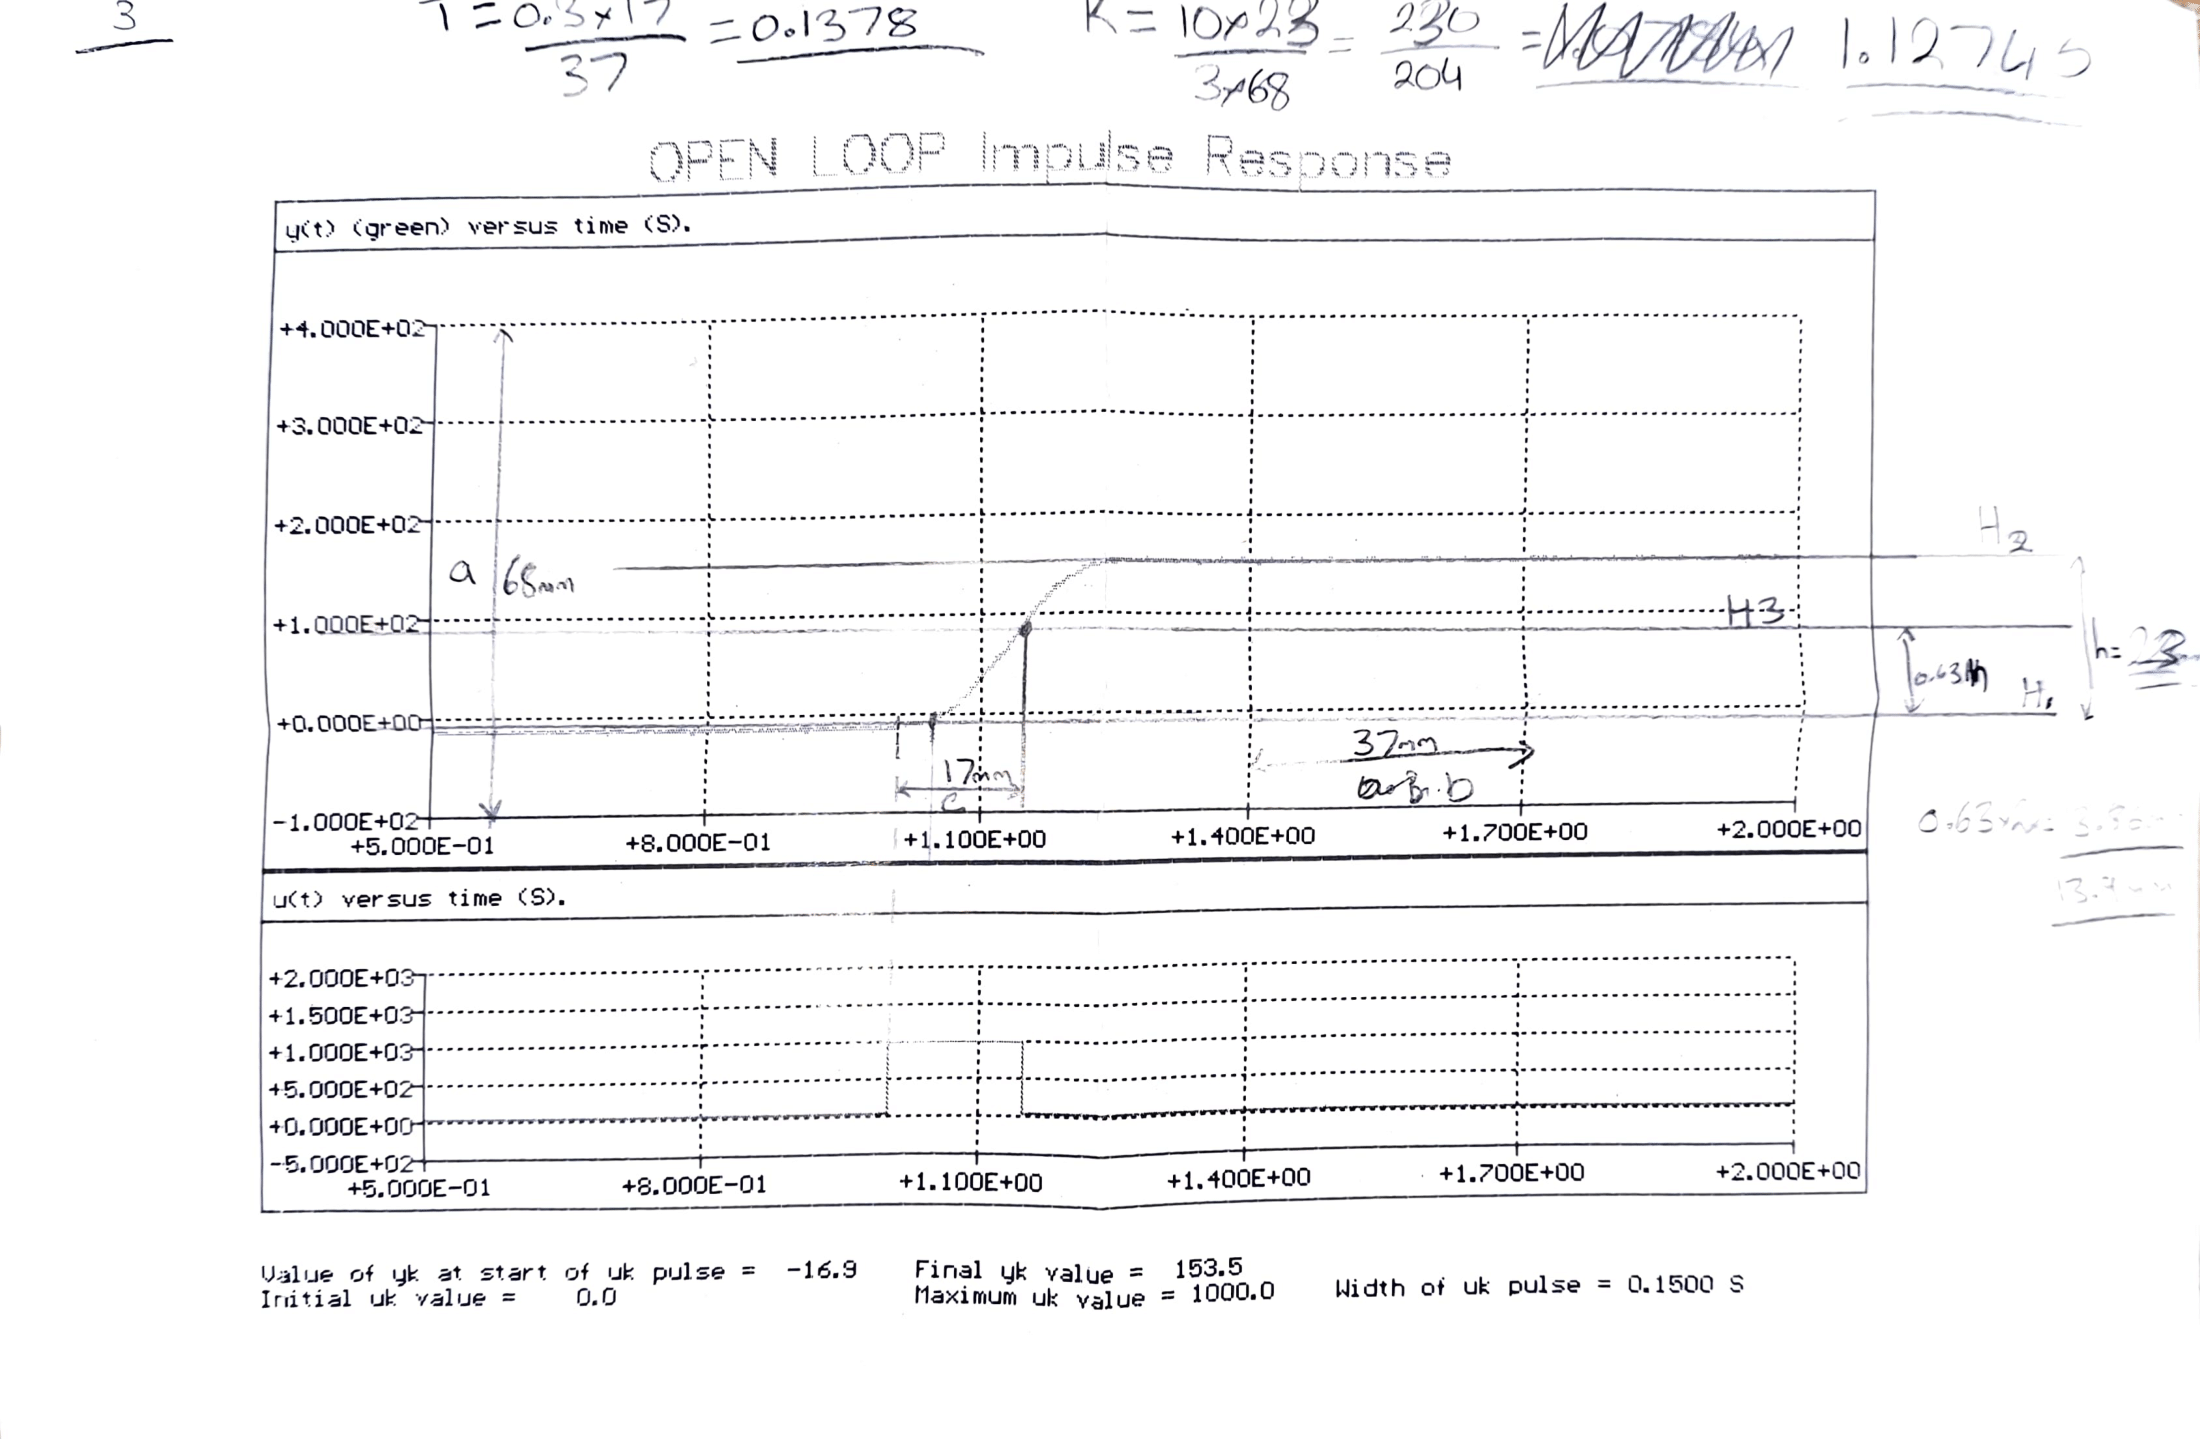
\includegraphics[width=1.1\textwidth]{pictures/task_1.png}
\end{figure}
Using this plot, values of $k$ and $T$ can be found using Equations 1.1 and 1.2. Where constants $a$, $b$, $c$ and $h$ are shown on Figure 1.1. 
\begin{equation}
    T = {{0.3c}\over{b}} \, ,
\end{equation}
\label{eq:1.1}
\myequations{Equation to find $T$.}
\begin{equation}
    k = {{10h}\over{3a}} \, ,
\end{equation}
\label{eq:1.2}
\myequations{Equation to find $k$.}
Time-constant T is in seconds, whereas k is a value for gain. The terms $a$, $b$, $c$ and $h$ were all measured in mm. When measuring the values are:
\begin{itemize}
    \item $a=64$
    \item $b=37$
    \item $c=17$
    \item $h=23$
\end{itemize}
Therefore, when applied to the equations for $k$ and $T$ the values obtained are:
\begin{equation}
    T = {{0.3\times17}\over{37}} = 0.1378  \, ,
\end{equation}
\label{eq:1.3}
\myequations{The value of $T$.}
\begin{equation}
    k = {{10\times23}\over{3\times64}} = 1.12745 \, ,
\end{equation}
\label{eq:1.4}
\myequations{The value of $k$.}
Now that the values of $k$ and $T$ have been obtained, the MATLAB script can be tuned to have the same performance as the real DC Servo it aims to simulate. 
\subsubsection{Step 2}
Step 2 focuses on only Digital-Proportional control of a DC Servo. For this step, the MATLAB simulation is run 4 times, producing 4 sets of results with sampling Times ($T_s$) of:
\begin{itemize}
    \item 0.01s
    \item 0.1s
    \item 0.5s
    \item 1.0s 
\end{itemize}
For each value of $T_s$ the following results are obtained:
\begin{itemize}
    \item An open-loop Transfer Function,
    \item Two values of $K_p$ (Proportional Gain) one for a damping ratio ($\zeta$) of 0.6 and one for a value of 1,
    \item Two root locus plots, one for each value of $\zeta$. 
    \item Two unit step responses, one for each value of $\zeta$. 
\end{itemize}
Table 1.1 displays all the values of $K_p$ and $G_{ol}$ with varying damping ratio ($\zeta$) and sampling time $T_s$. 
\begin{table}[H]
    \centering
    \caption{The values of Proportional Gain $K_p$ and $G_{ol}$ with varying Damping Ratio and Sampling Time.}
    \label{tab:task2_gain_table}
    \begin{tabular}{@{}cccl@{}}
    \toprule
    \multicolumn{1}{l}{}         & \textbf{Damping Ratio = 0.6} & \textbf{Damping Ratio = 1} & \multicolumn{1}{c}{\textbf{Transfer Function}}                    \\ \midrule
    \textbf{Sampling Time $T_s$} & $K_p$                        & $K_p$                      & \multicolumn{1}{c}{$G_{ol}(z)$}                                      \\
    0.01                         & 4.2518                       & 1.5801                     & ${{0.0003994 z + 0.0003898}\over{z^2-1.93z+0.93}}$      \\
    0.1                          & 2.9833                       & 1.3470                     & ${{0.03258 z + 0.0256}\over{z^2 - 1.484 z + 0.484}}$    \\
    0.5                          & 1.3548                       & 0.7494                     & ${{0.4125 z + 0.1363}\over{z^2 - 1.027 z + 0.02656}}$   \\
    1.0                          & 0.8609                       & 0.4715                     & ${{0.9722 z + 0.1545}\over{z^2 - 1.001 z + 0.0007053}}$ \\ \bottomrule
\end{tabular}
\end{table}
Its important to note that as the sampling time and damping ratio increases, the value of the proportional gain decreases. The same can be said for the poles of the transfer function. Each transfer function has a pole of 1, but the value of the additional pole decreases as the sampling time increases.
The root locus plots for sampling time 0.01 can be found below in Figure 1.2 (damping ratio 0.6) and Figure 1.3 (damping ratio 1). 
\begin{figure}[H]
    \caption{$T_s = 0.01$: Root Locus Plot when the damping ratio is 0.6}
    \label{fig:0.01_Ts_damping_0.6}
    \centering
    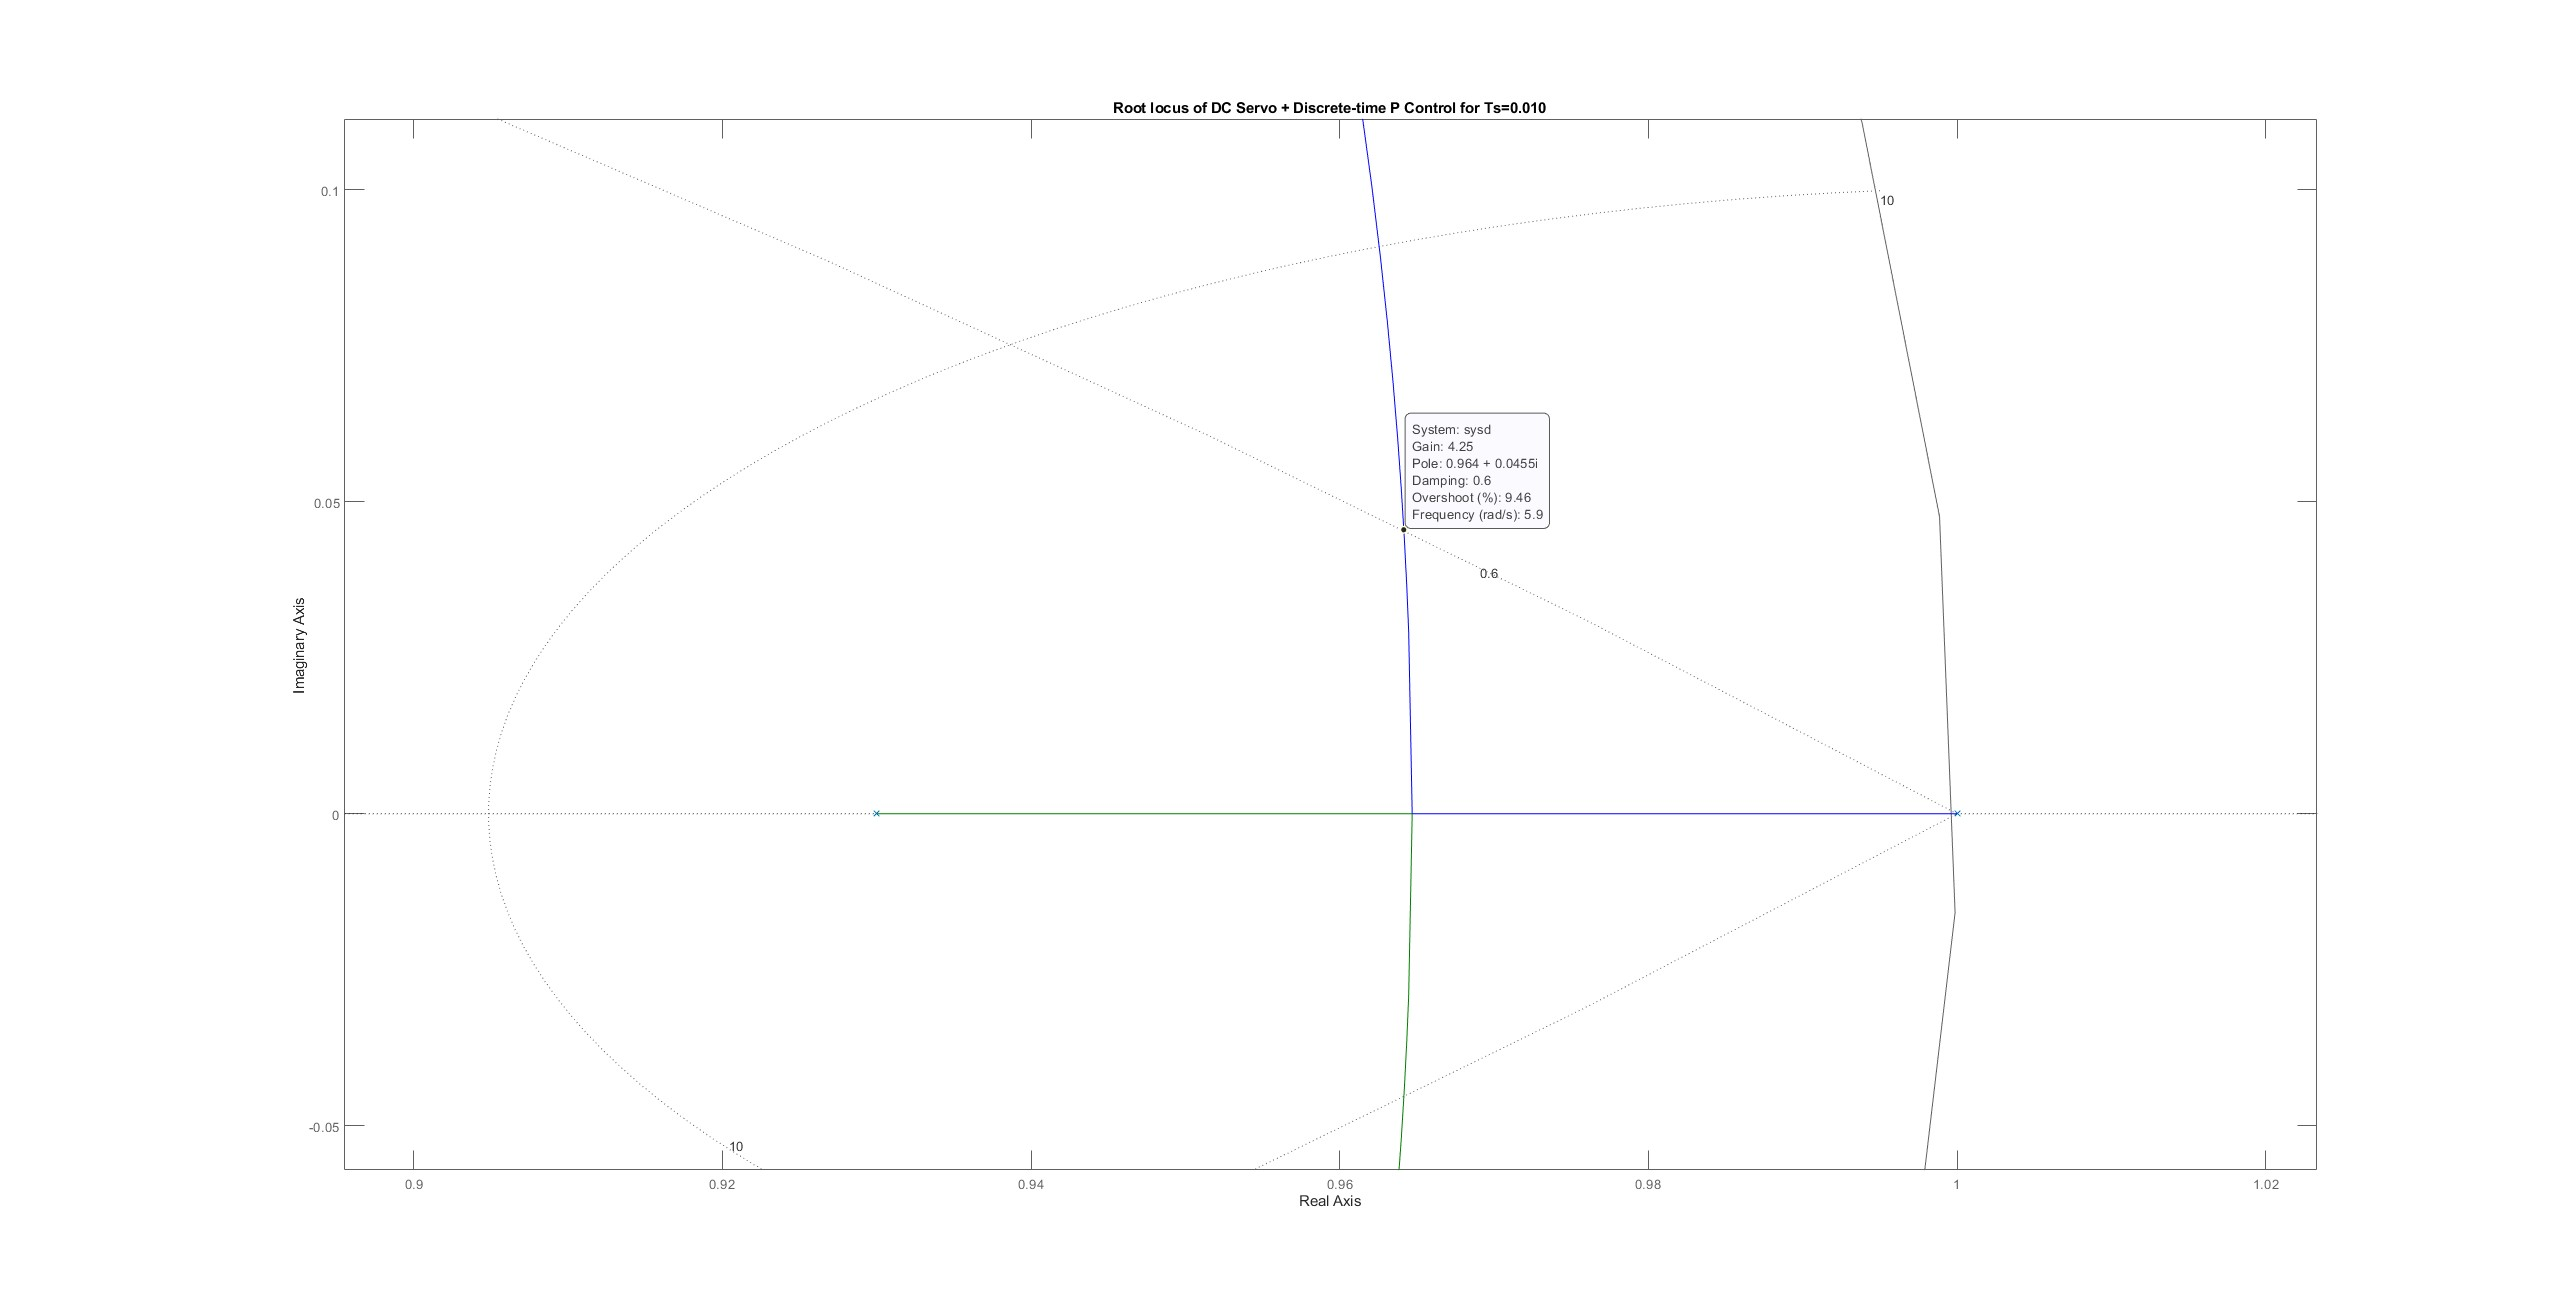
\includegraphics[width=1.1\textwidth]{pictures/task2_0.01_damping_0.6.jpg}
\end{figure}
\begin{figure}[H]
    \caption{$T_s = 0.01$: Root Locus Plot when the damping ratio is 1}
    \label{fig:0.01_Ts_damping_1}
    \centering
    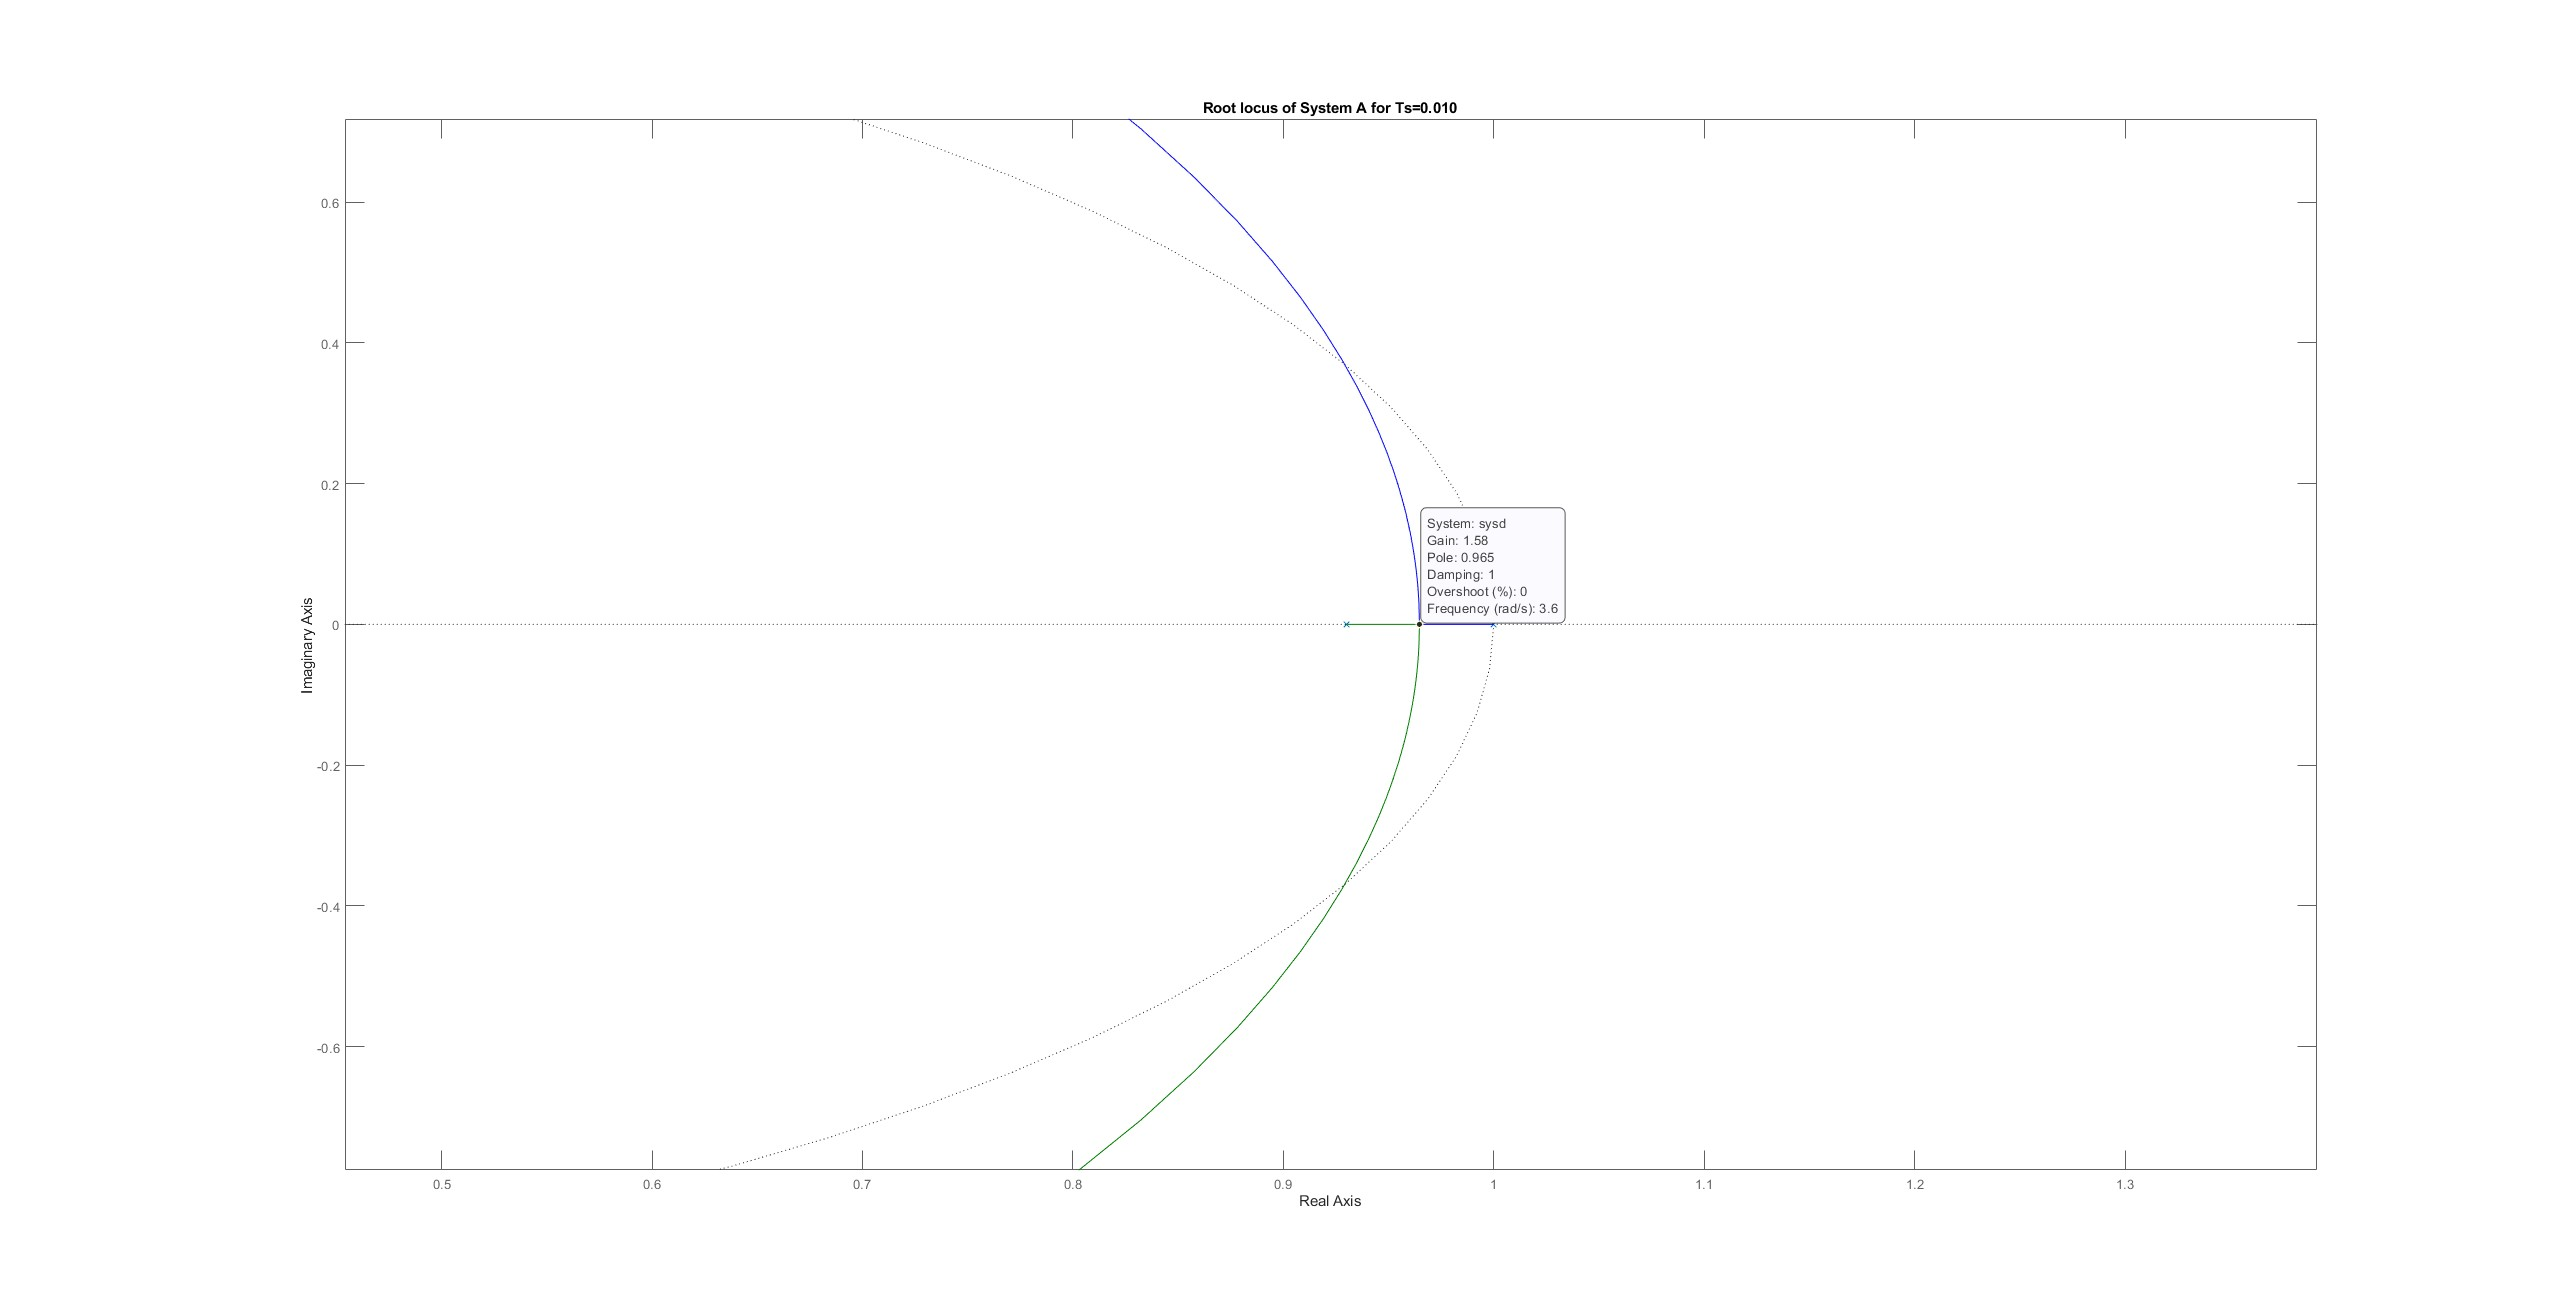
\includegraphics[width=1.1\textwidth]{pictures/task2_0.01_damping_1.jpg}
\end{figure}
The root locus plots for sampling time 0.1 can be found below in Figure 1.4 (damping ratio 0.6) and Figure 1.5 (damping ratio 1). 
\begin{figure}[H]
    \caption{$T_s = 0.1$: Root Locus Plot when the damping ratio is 0.6}
    \label{fig:0.1_Ts_damping_0.6}
    \centering
    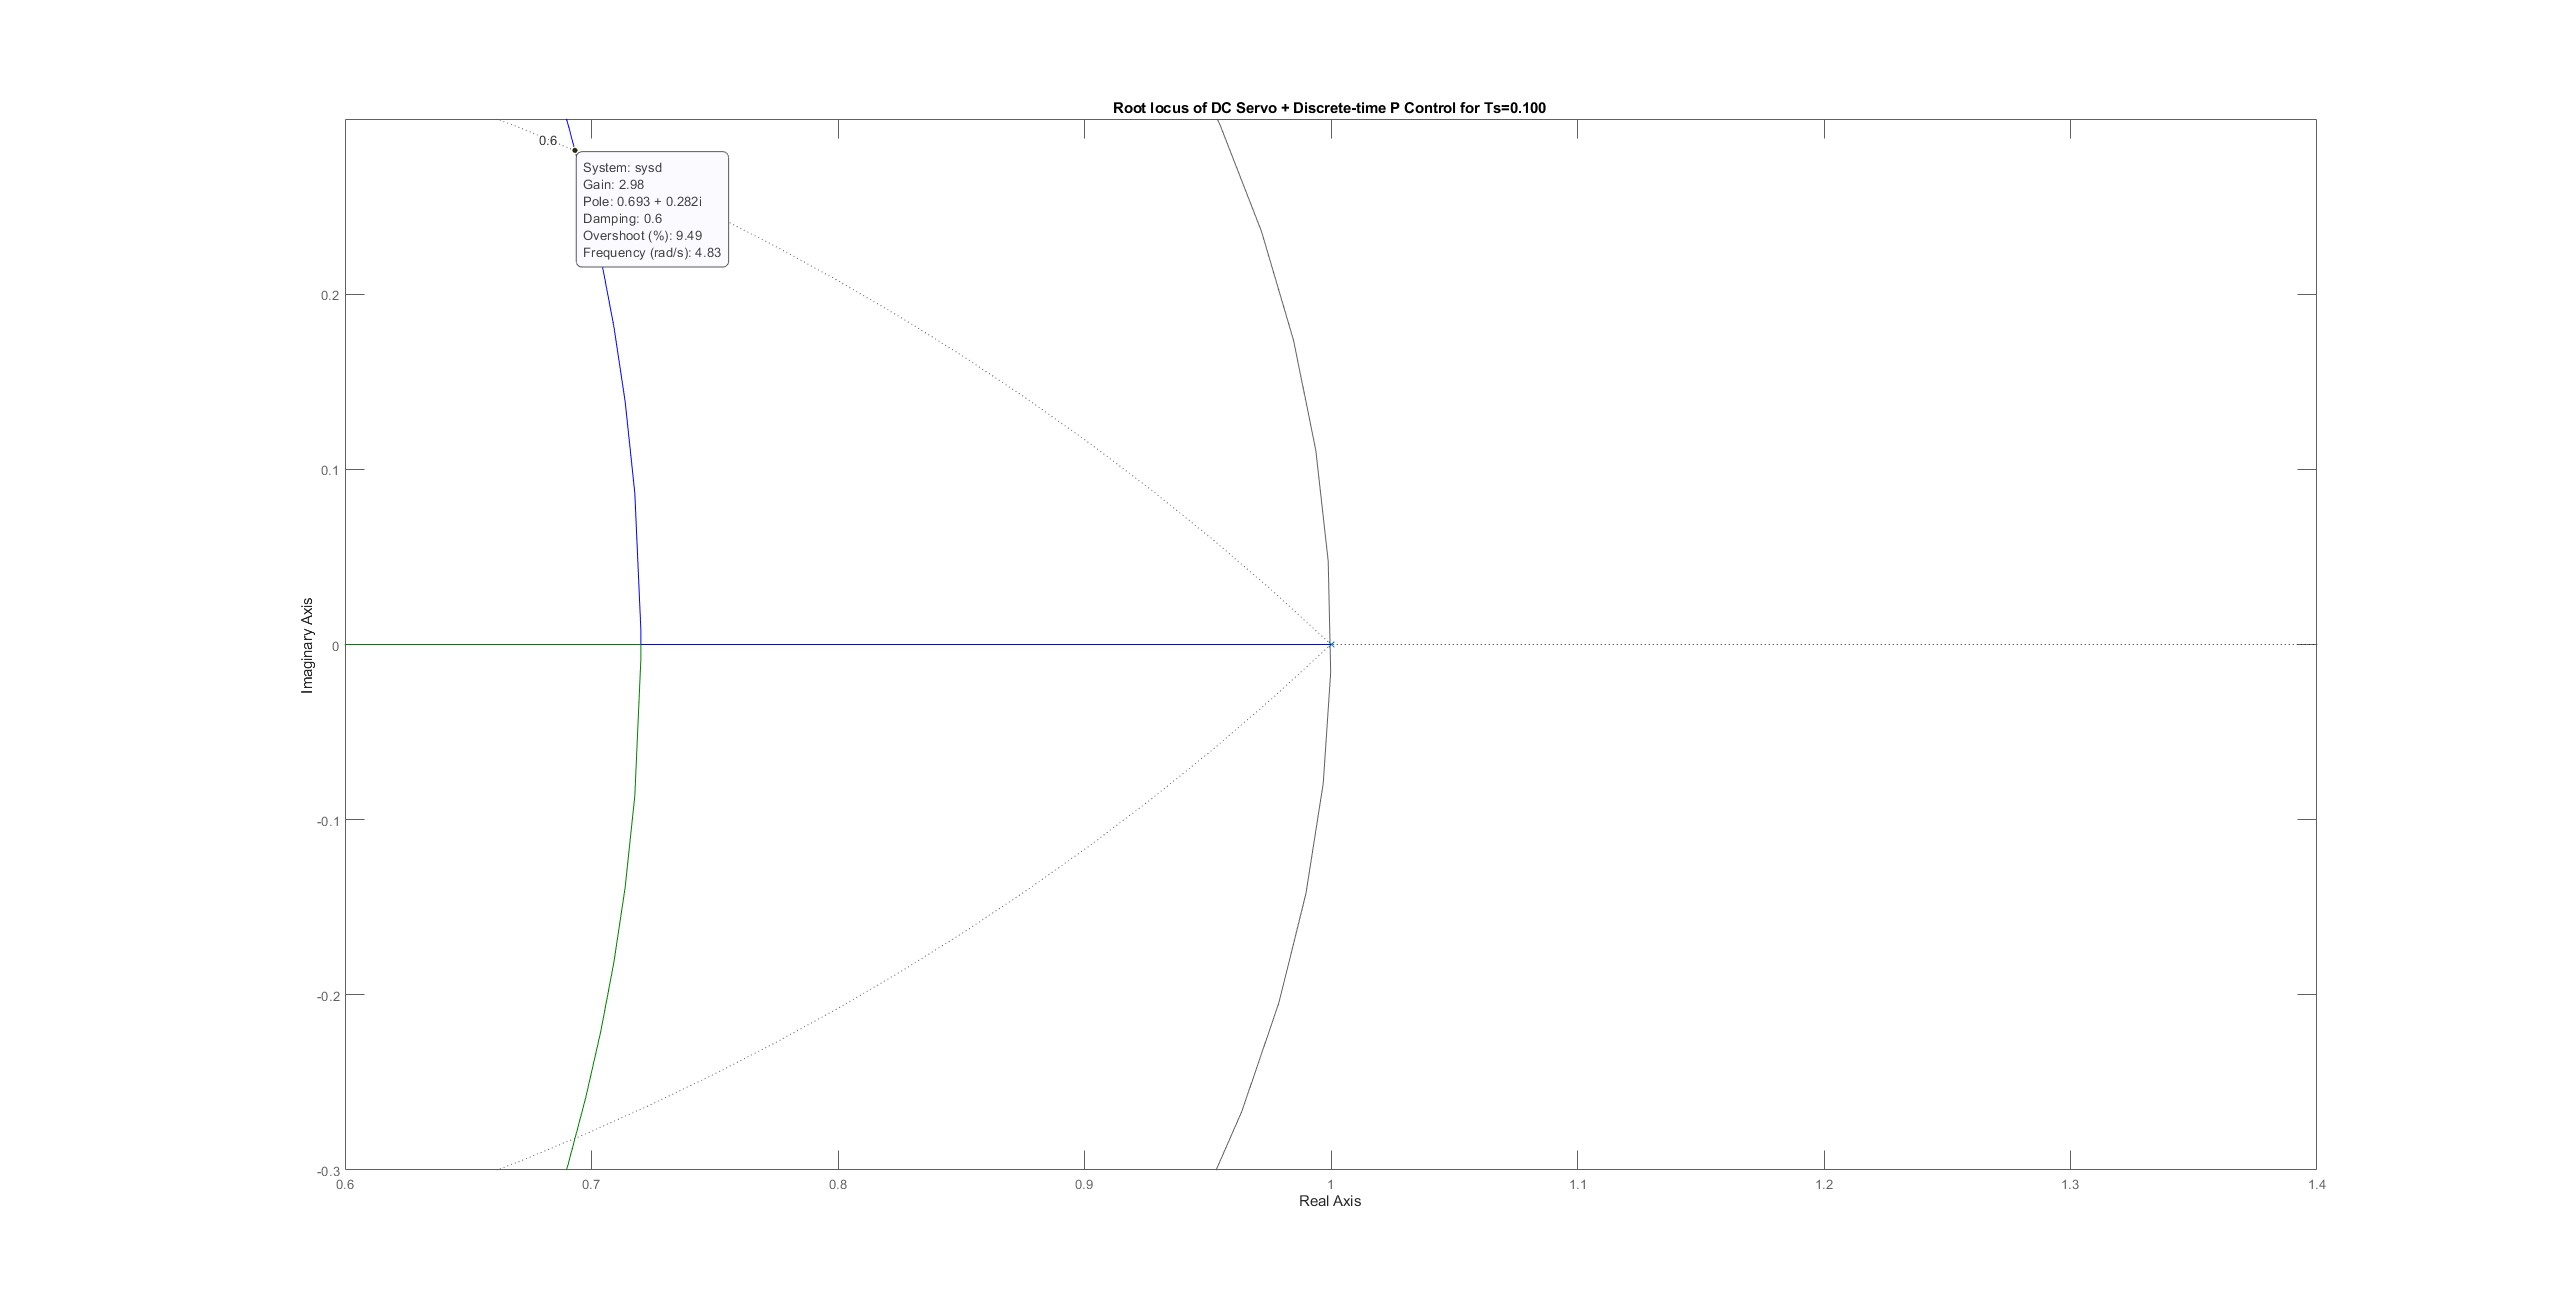
\includegraphics[width=1.1\textwidth]{pictures/task2_0.1_damping_0.6.jpg}
\end{figure}
\begin{figure}[H]
    \caption{$T_s = 0.1$: Root Locus Plot when the damping ratio is 1}
    \label{fig:0.1_Ts_damping_1}
    \centering
    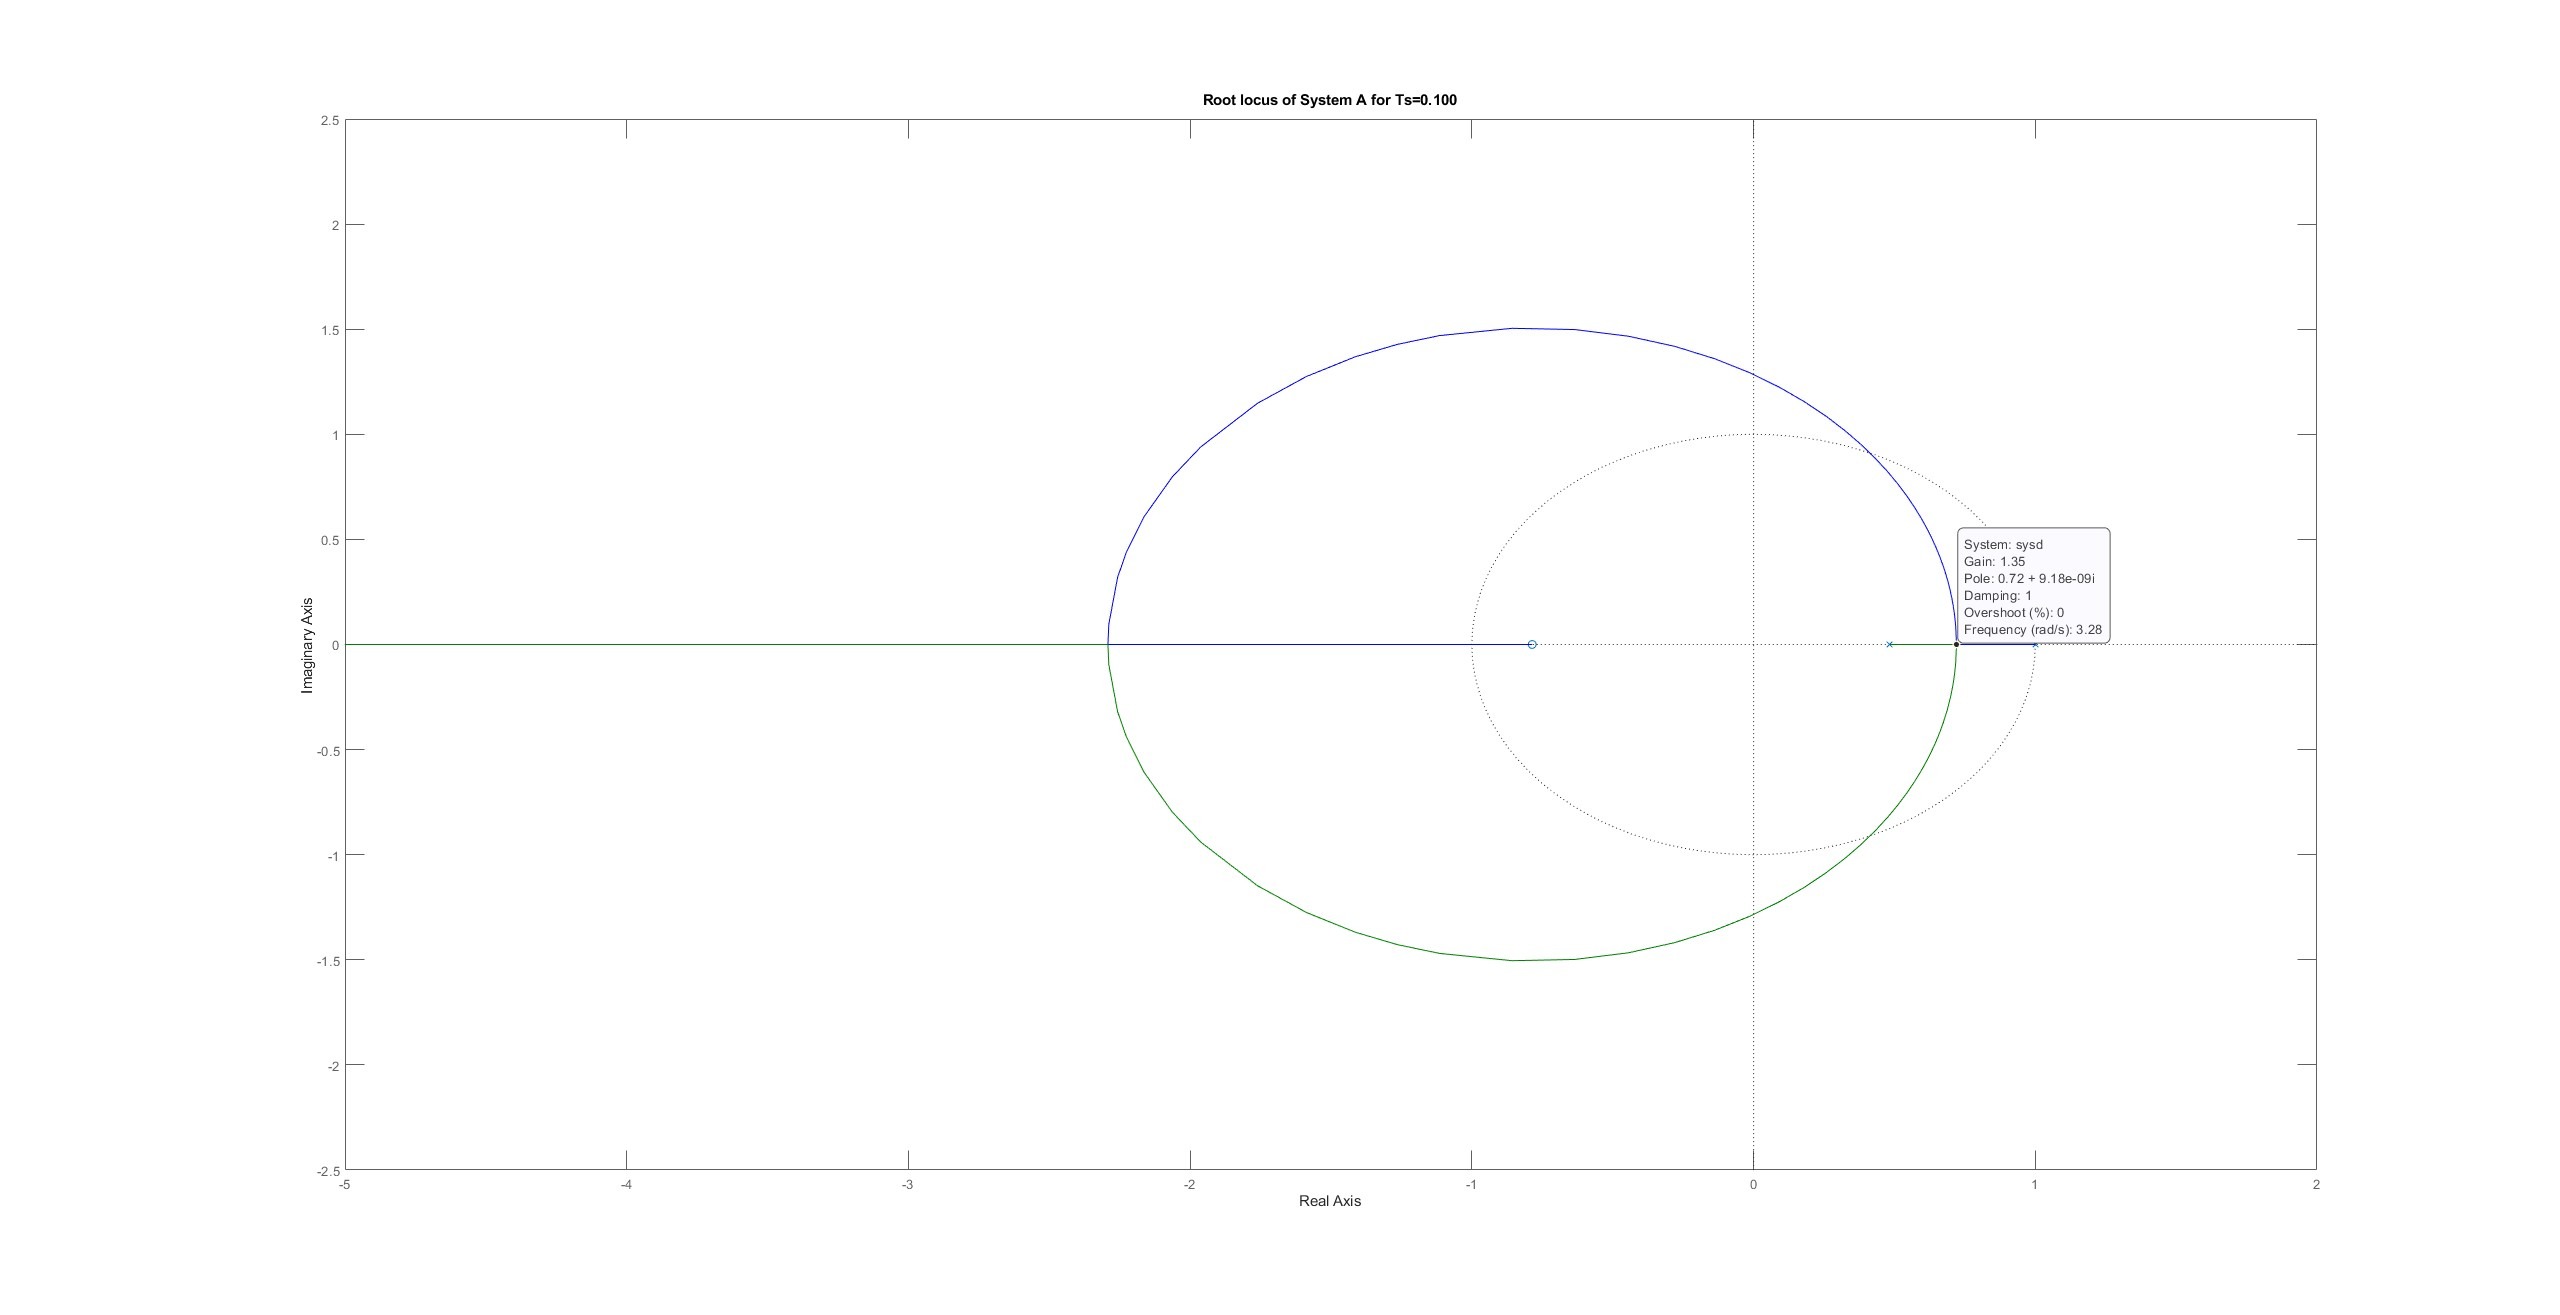
\includegraphics[width=1.1\textwidth]{pictures/task2_0.1_damping_1.jpg}
\end{figure}
The root locus plots for sampling time 0.5 can be found below in Figure 1.6 (damping ratio 0.6) and Figure 1.7 (damping ratio 1). 
\begin{figure}[H]
    \caption{$T_s = 0.5$: Root Locus Plot when the damping ratio is 0.6}
    \label{fig:0.5_Ts_damping_0.6}
    \centering
    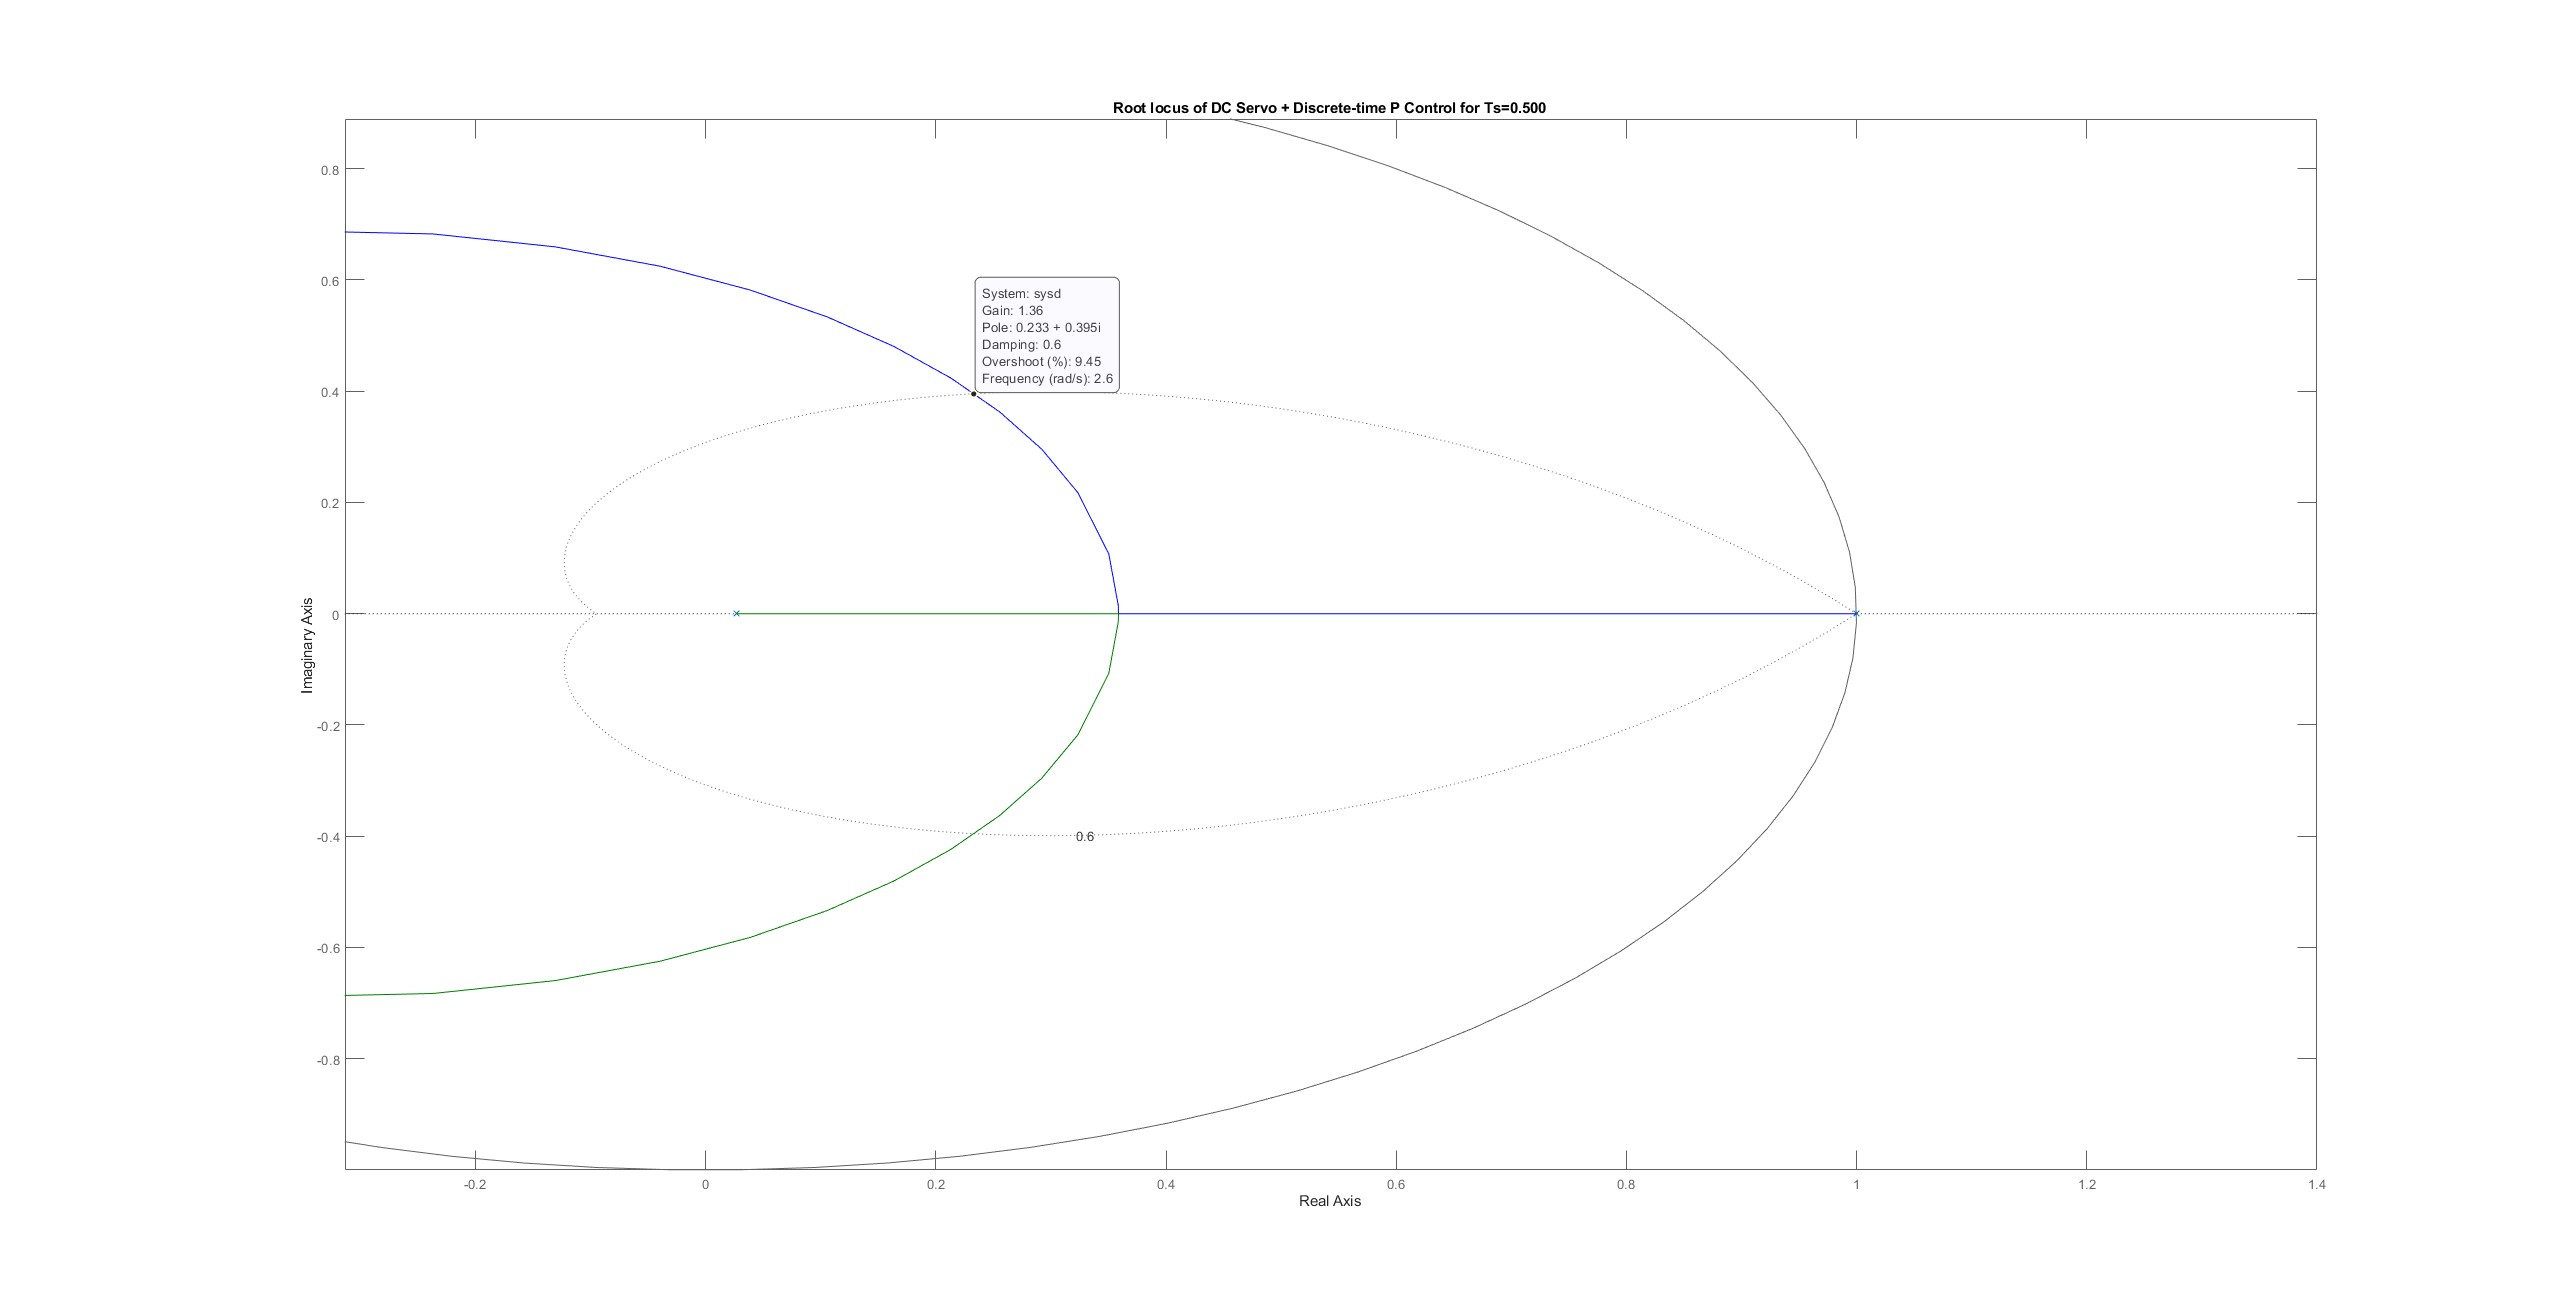
\includegraphics[width=1.1\textwidth]{pictures/task2_0.5_damping_0.6.jpg}
\end{figure}
\begin{figure}[H]
    \caption{$T_s = 0.5$: Root Locus Plot when the damping ratio is 1}
    \label{fig:0.5_Ts_damping_1}
    \centering
    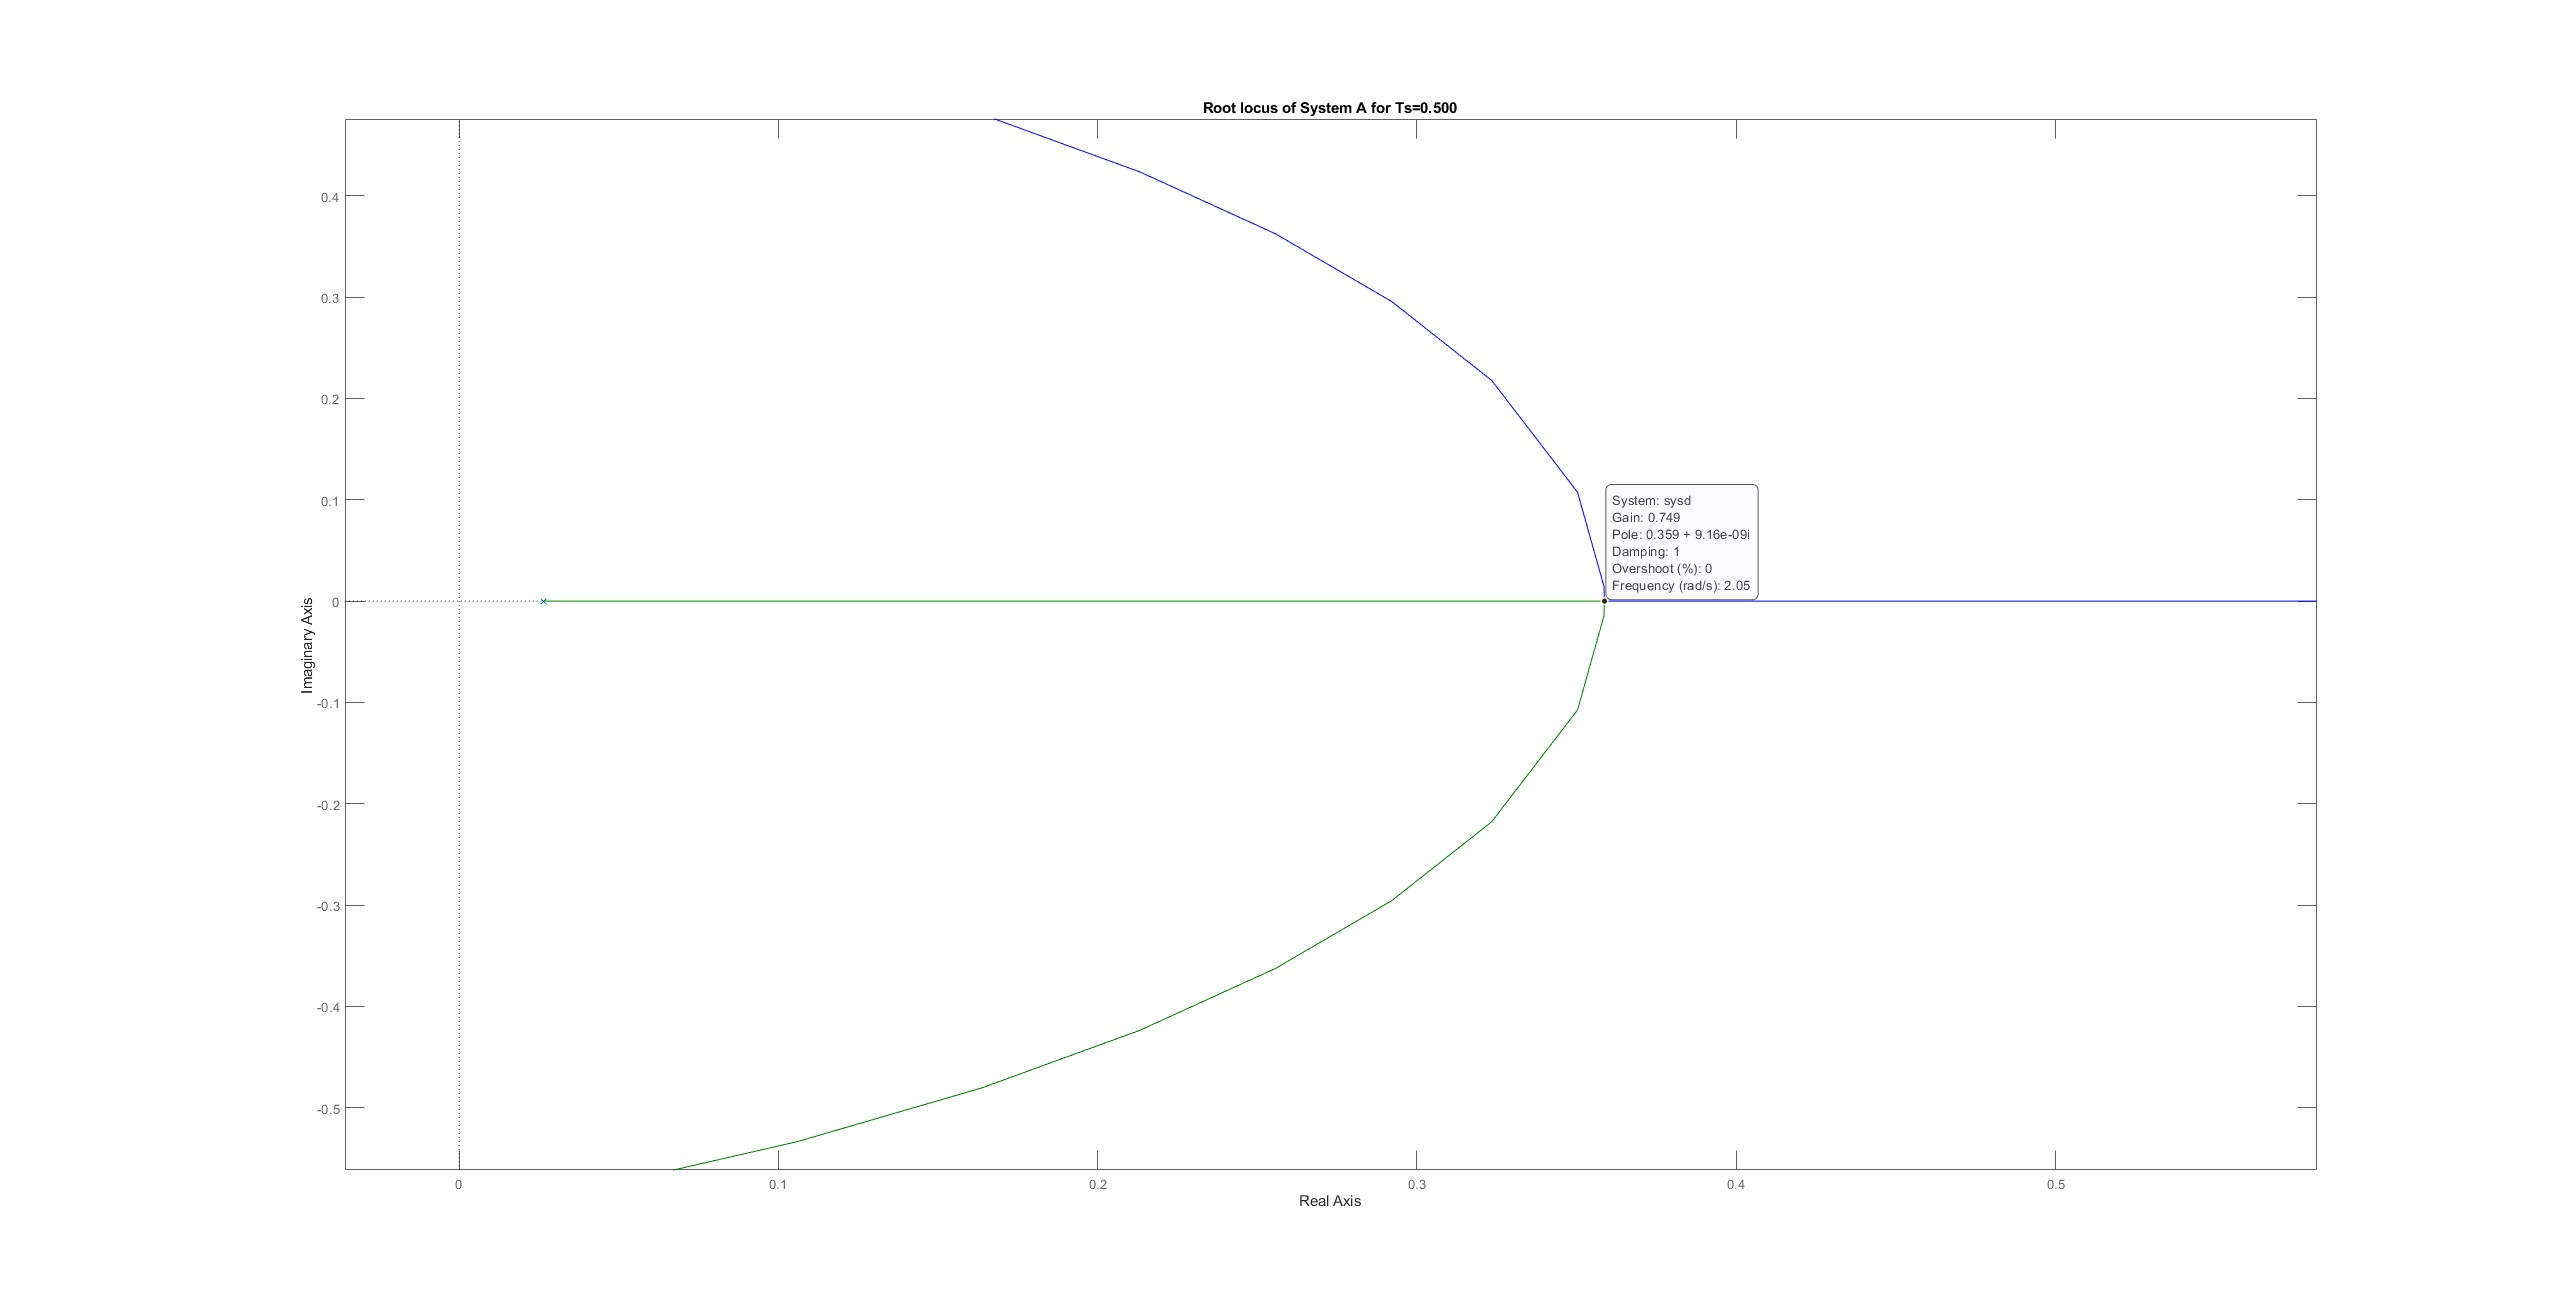
\includegraphics[width=1.1\textwidth]{pictures/task2_0.5_damping_1.jpg}
\end{figure}
The root locus plots for sampling time 1.0 can be found below in Figure 1.8 (damping ratio 0.6) and Figure 1.9 (damping ratio 1). 
\begin{figure}[H]
    \caption{$T_s = 1.0$: Root Locus Plot when the damping ratio is 0.6}
    \label{fig:1.0_Ts_damping_0.6}
    \centering
    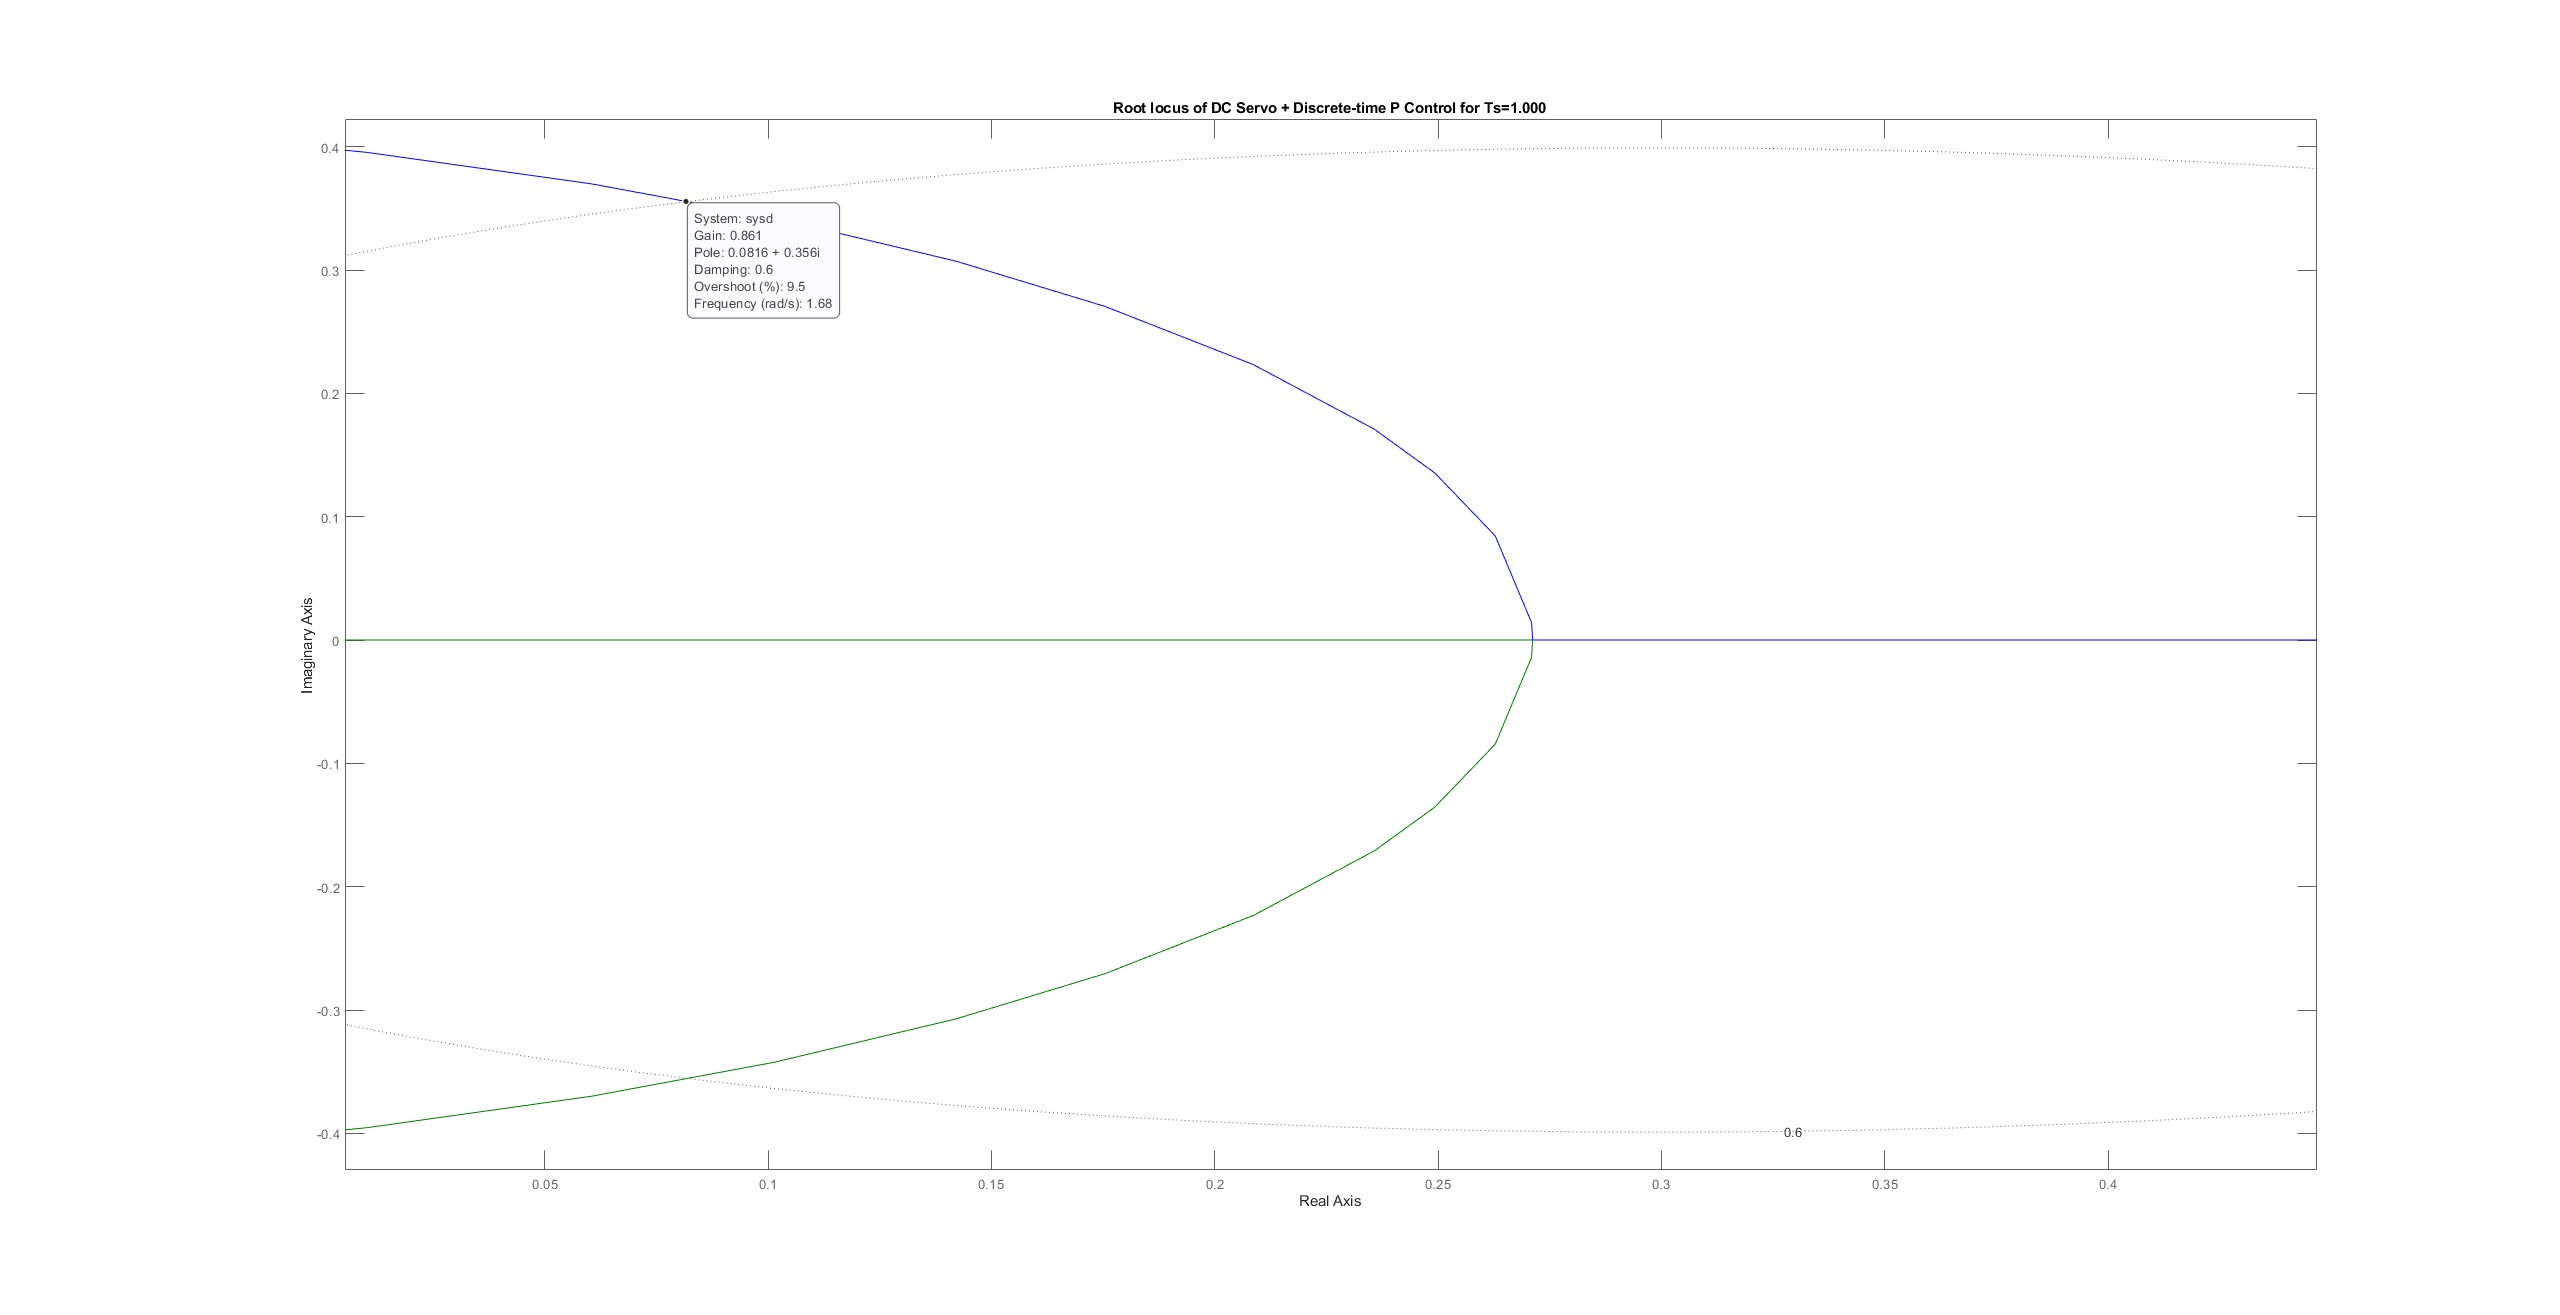
\includegraphics[width=1.1\textwidth]{pictures/task2_1.0_damping_0.6.jpg}
\end{figure}
\begin{figure}[H]
    \caption{$T_s = 1.0$: Root Locus Plot when the damping ratio is 1}
    \label{fig:1.0_Ts_damping_1}
    \centering
    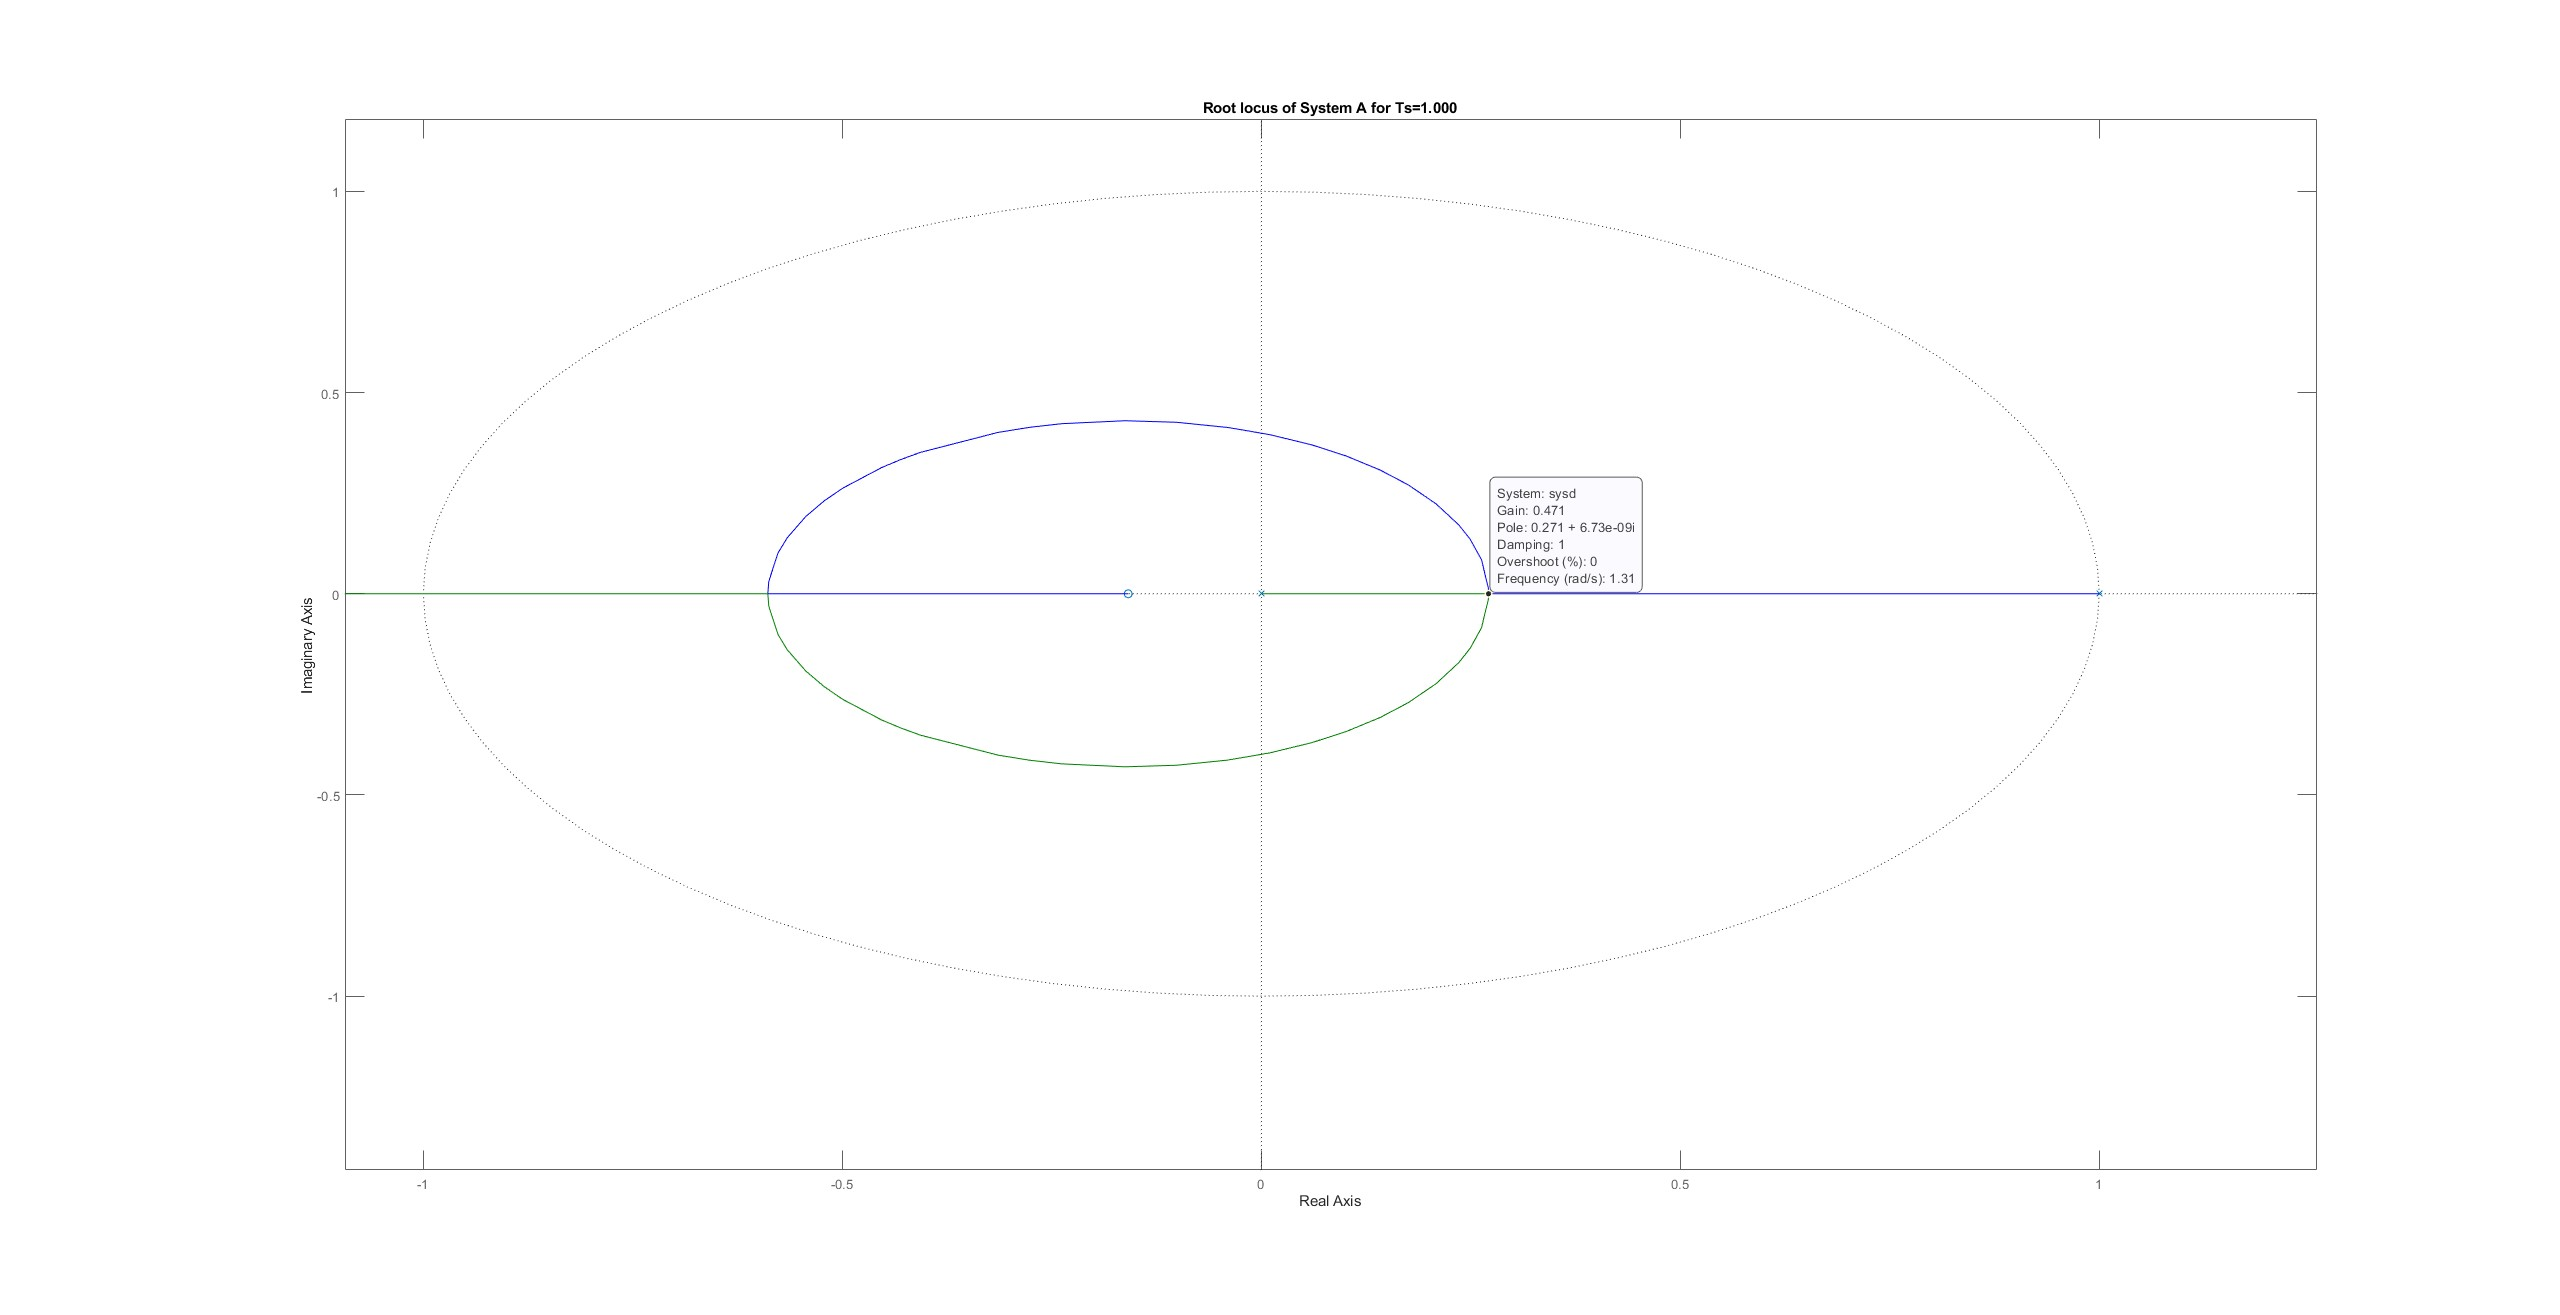
\includegraphics[width=1.1\textwidth]{pictures/task2_1.0_damping_1.jpg}
\end{figure}
Finally, now that the root locus design has been completed, the step responses for each sampling time and proportional gain can be produced. Figures 1.10 and 1.11 show the step response for gain 4.2518 and 1.1275 respectively. 
\begin{figure}[H]
    \caption{$T_s = 0.01$: Step Response when the gain is 4.2518}
    \label{fig:0.01_Ts_step_response_1}
    \centering
    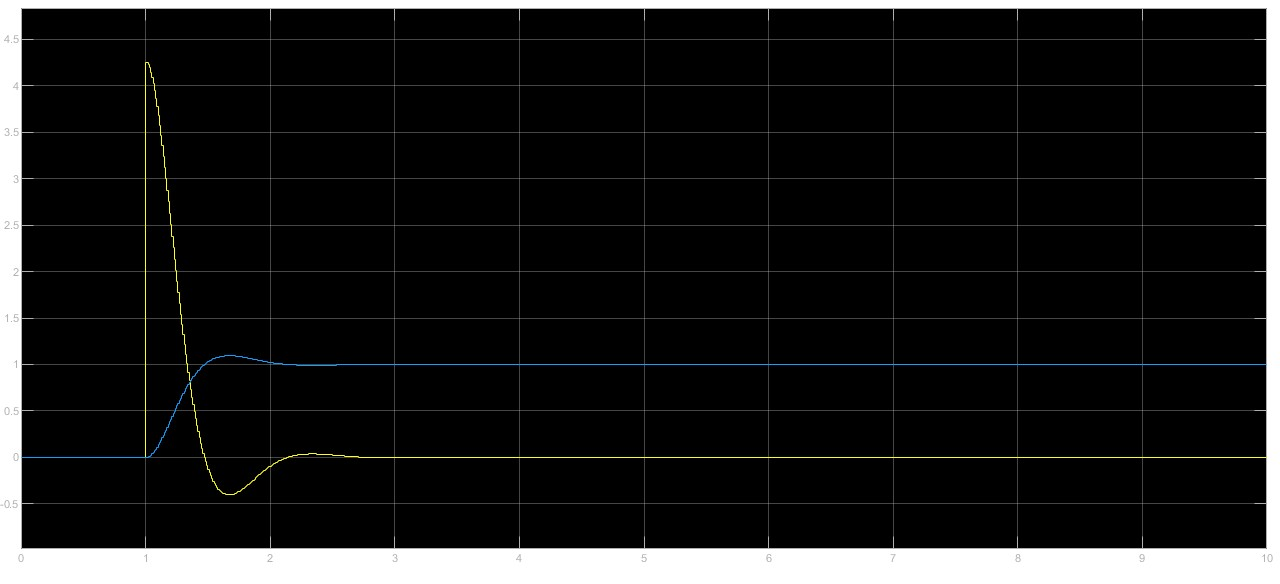
\includegraphics[width=1.1\textwidth]{pictures/task2_0.01_step_response_1.jpg}
\end{figure}
This plot shows a response that has been underdamped slightly, due to the overshoot seen in the response.
\begin{figure}[H]
    \caption{$T_s = 0.01$: Step Response when the gain is 1.1275}
    \label{fig:0.01_Ts_step_response_2}
    \centering
    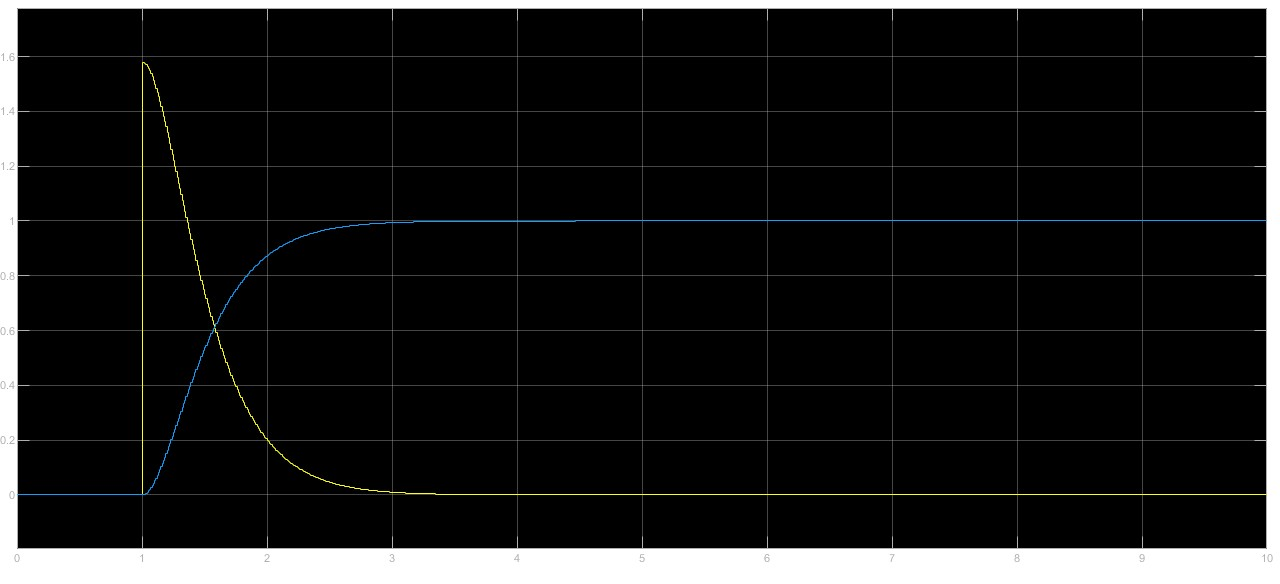
\includegraphics[width=1.1\textwidth]{pictures/task2_0.01_step_response_2.jpg}
\end{figure}
This plot shows a response that could be described as critically damped, as the response effectively returns to the original value. 

Figures 1.12 and 1.13 show the step response for gain 2.9833 and 1.3470 respectively for a sampling time of 0.1 seconds.
\begin{figure}[H]
    \caption{$T_s = 0.1$: Step Response when the gain is 2.9833}
    \label{fig:0.1_Ts_step_response_1}
    \centering
    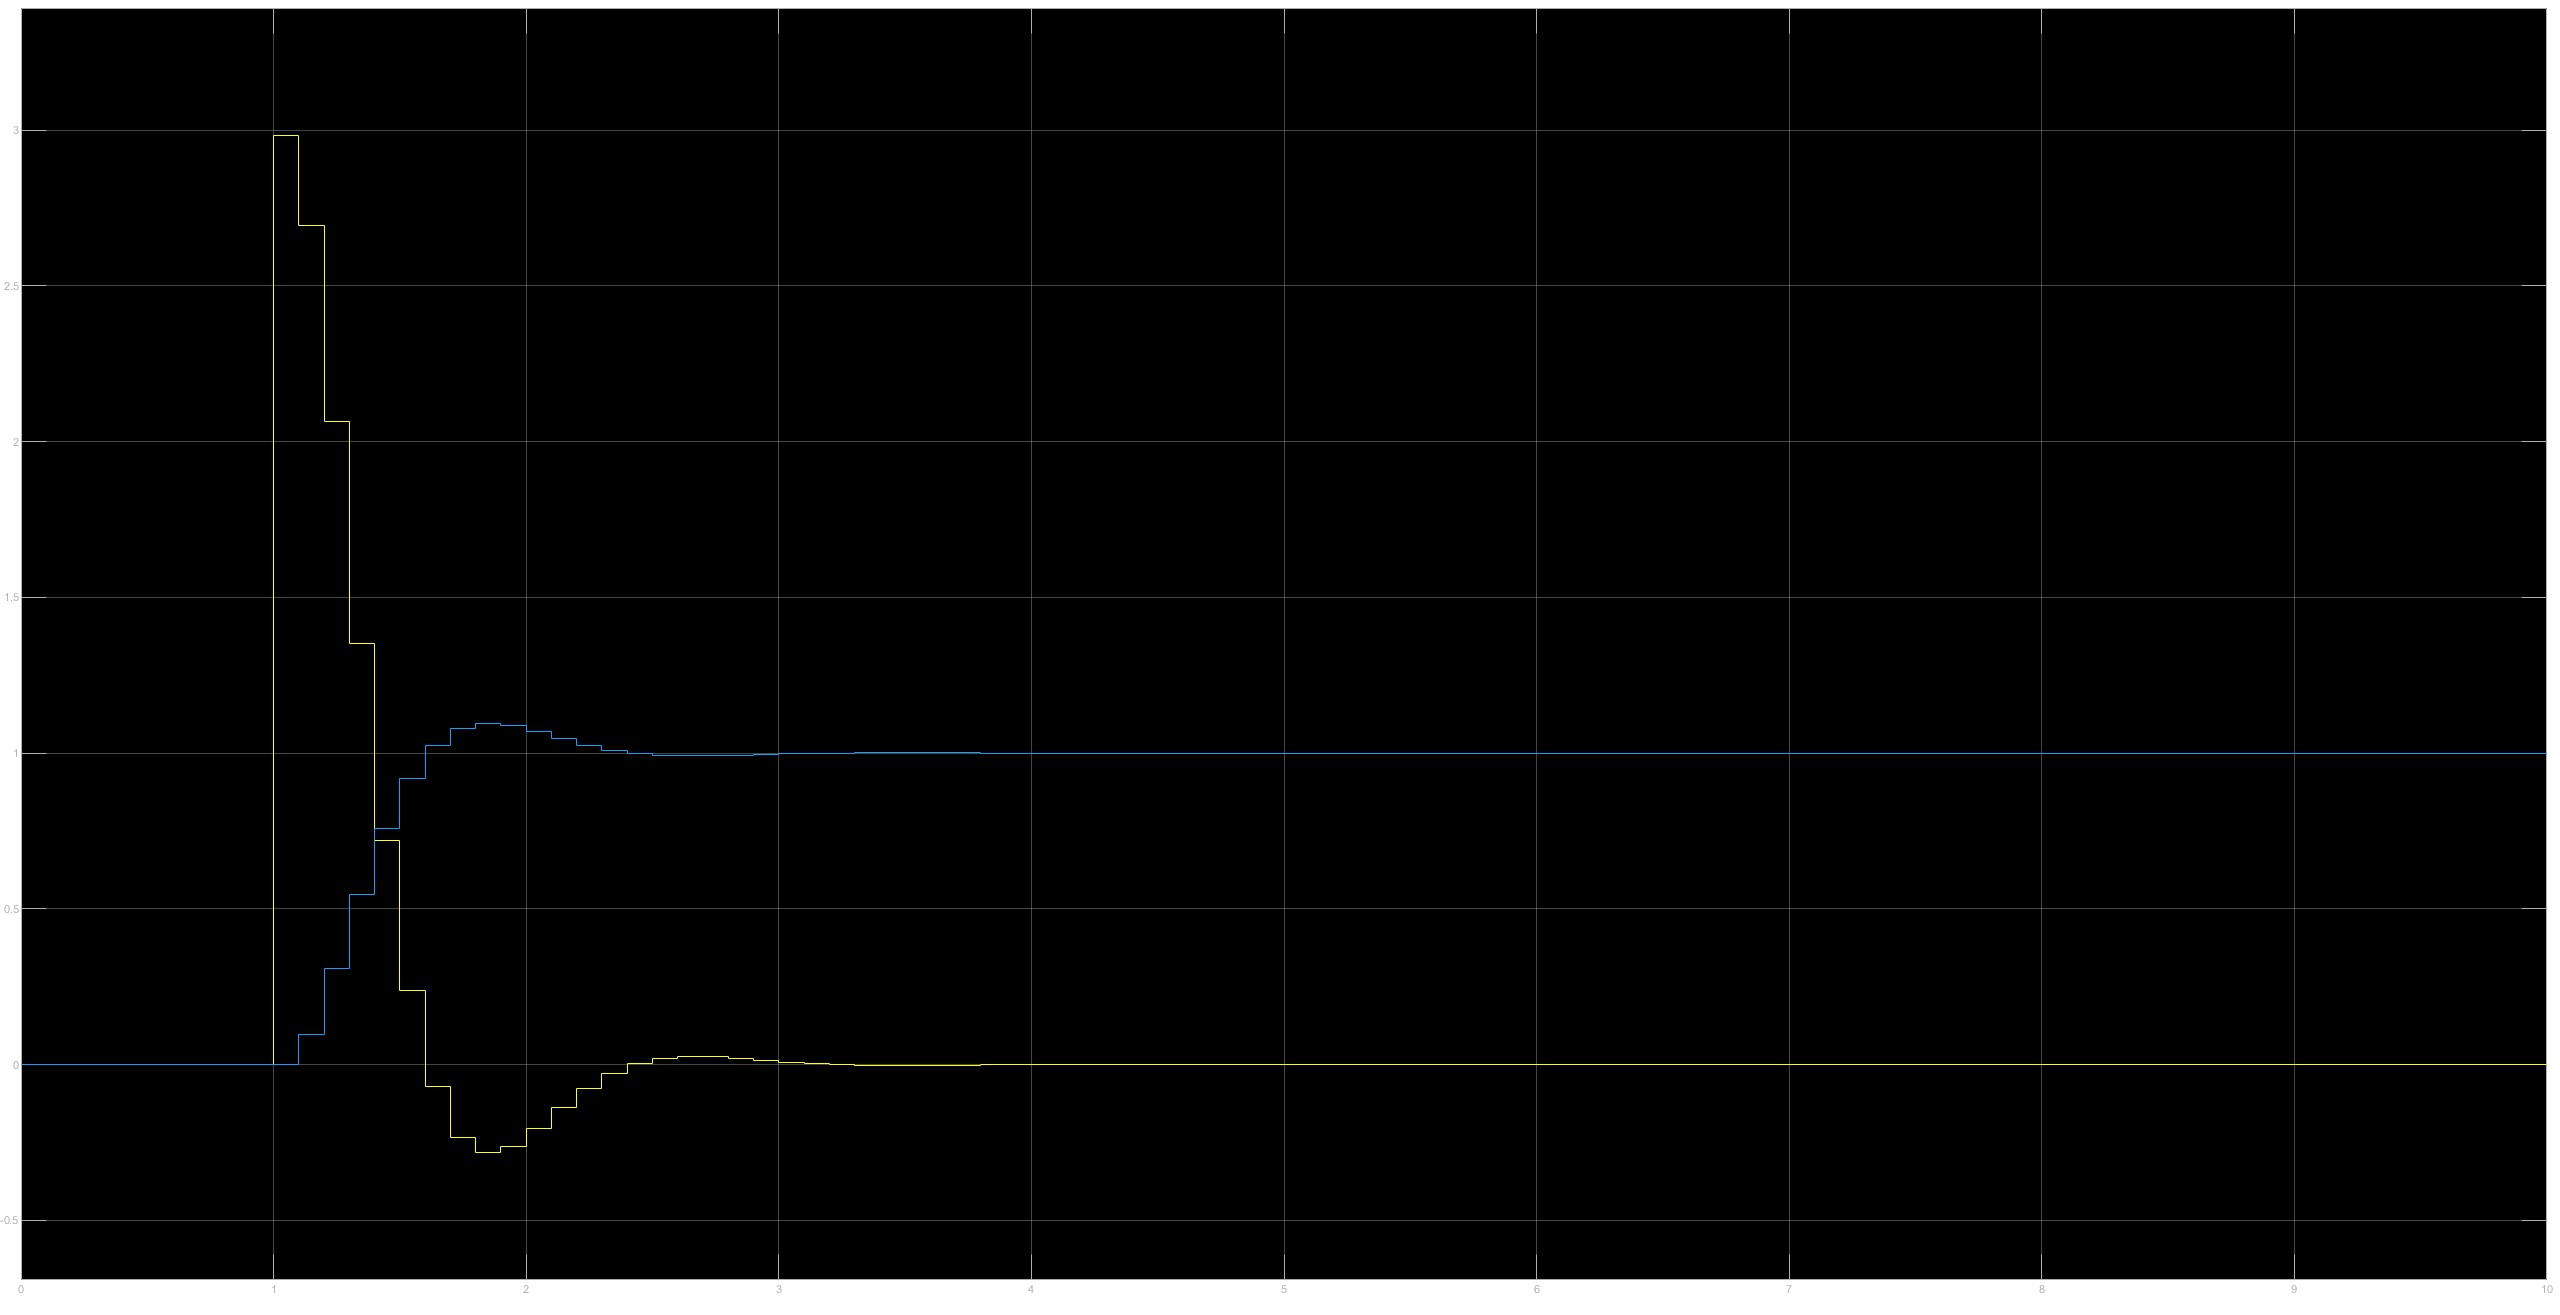
\includegraphics[width=1.1\textwidth]{pictures/task2_0.1_step_response_1.jpg}
\end{figure}
The longer sampling time has resulted in the blocky appearance of this response, although the general nature of the response is the same as in Figure 1.10.
\begin{figure}[H]
    \caption{$T_s = 0.1$: Step Response when the gain is 1.3470}
    \label{fig:0.1_Ts_step_response_2}
    \centering
    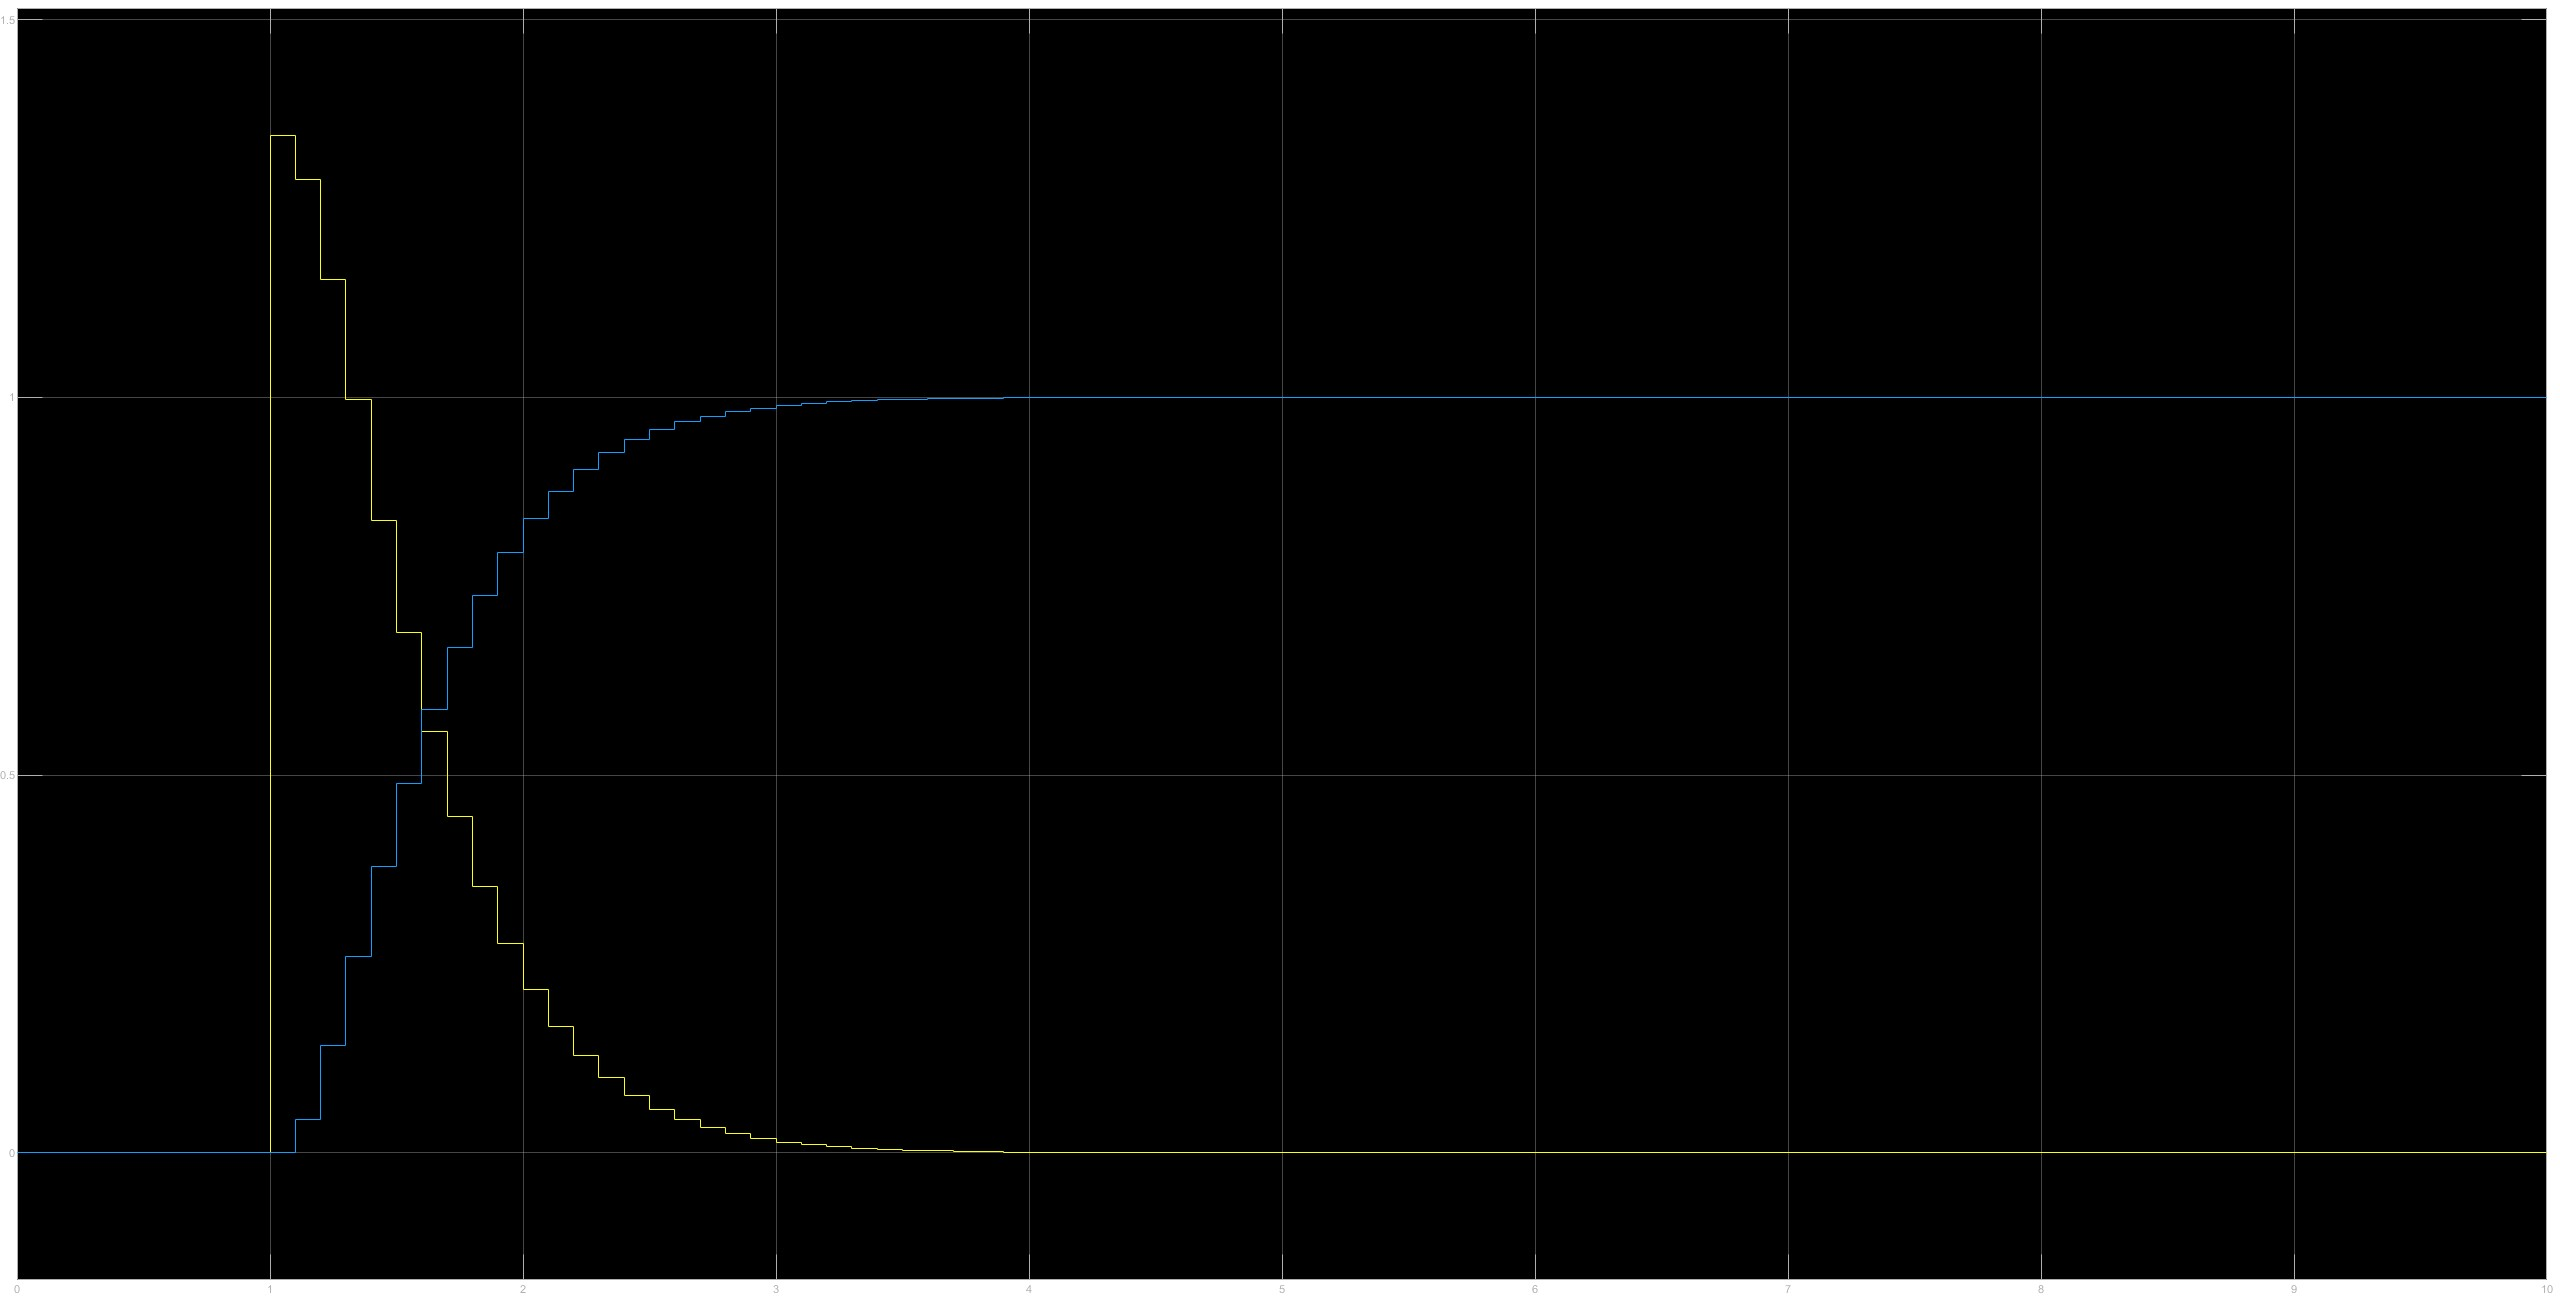
\includegraphics[width=1.1\textwidth]{pictures/task2_0.1_step_response_2.jpg}
\end{figure}
The longer sampling time has resulted in the blocky appearance of this response, although the general nature of the response is the same as in Figure 1.11.

In fact, the same is true for sampling times of 0.5 and 1 seconds. The responses relating to 0.5 seconds can be seen in Figures 1.13 and 1.14 and the figures relating to 1.0 seconds can be seen in Figures 1.15 and 1.16.
\begin{figure}[H]
    \caption{$T_s = 0.5$: Step Response when the gain is 1.3548}
    \label{fig:0.5_Ts_step_response_2}
    \centering
    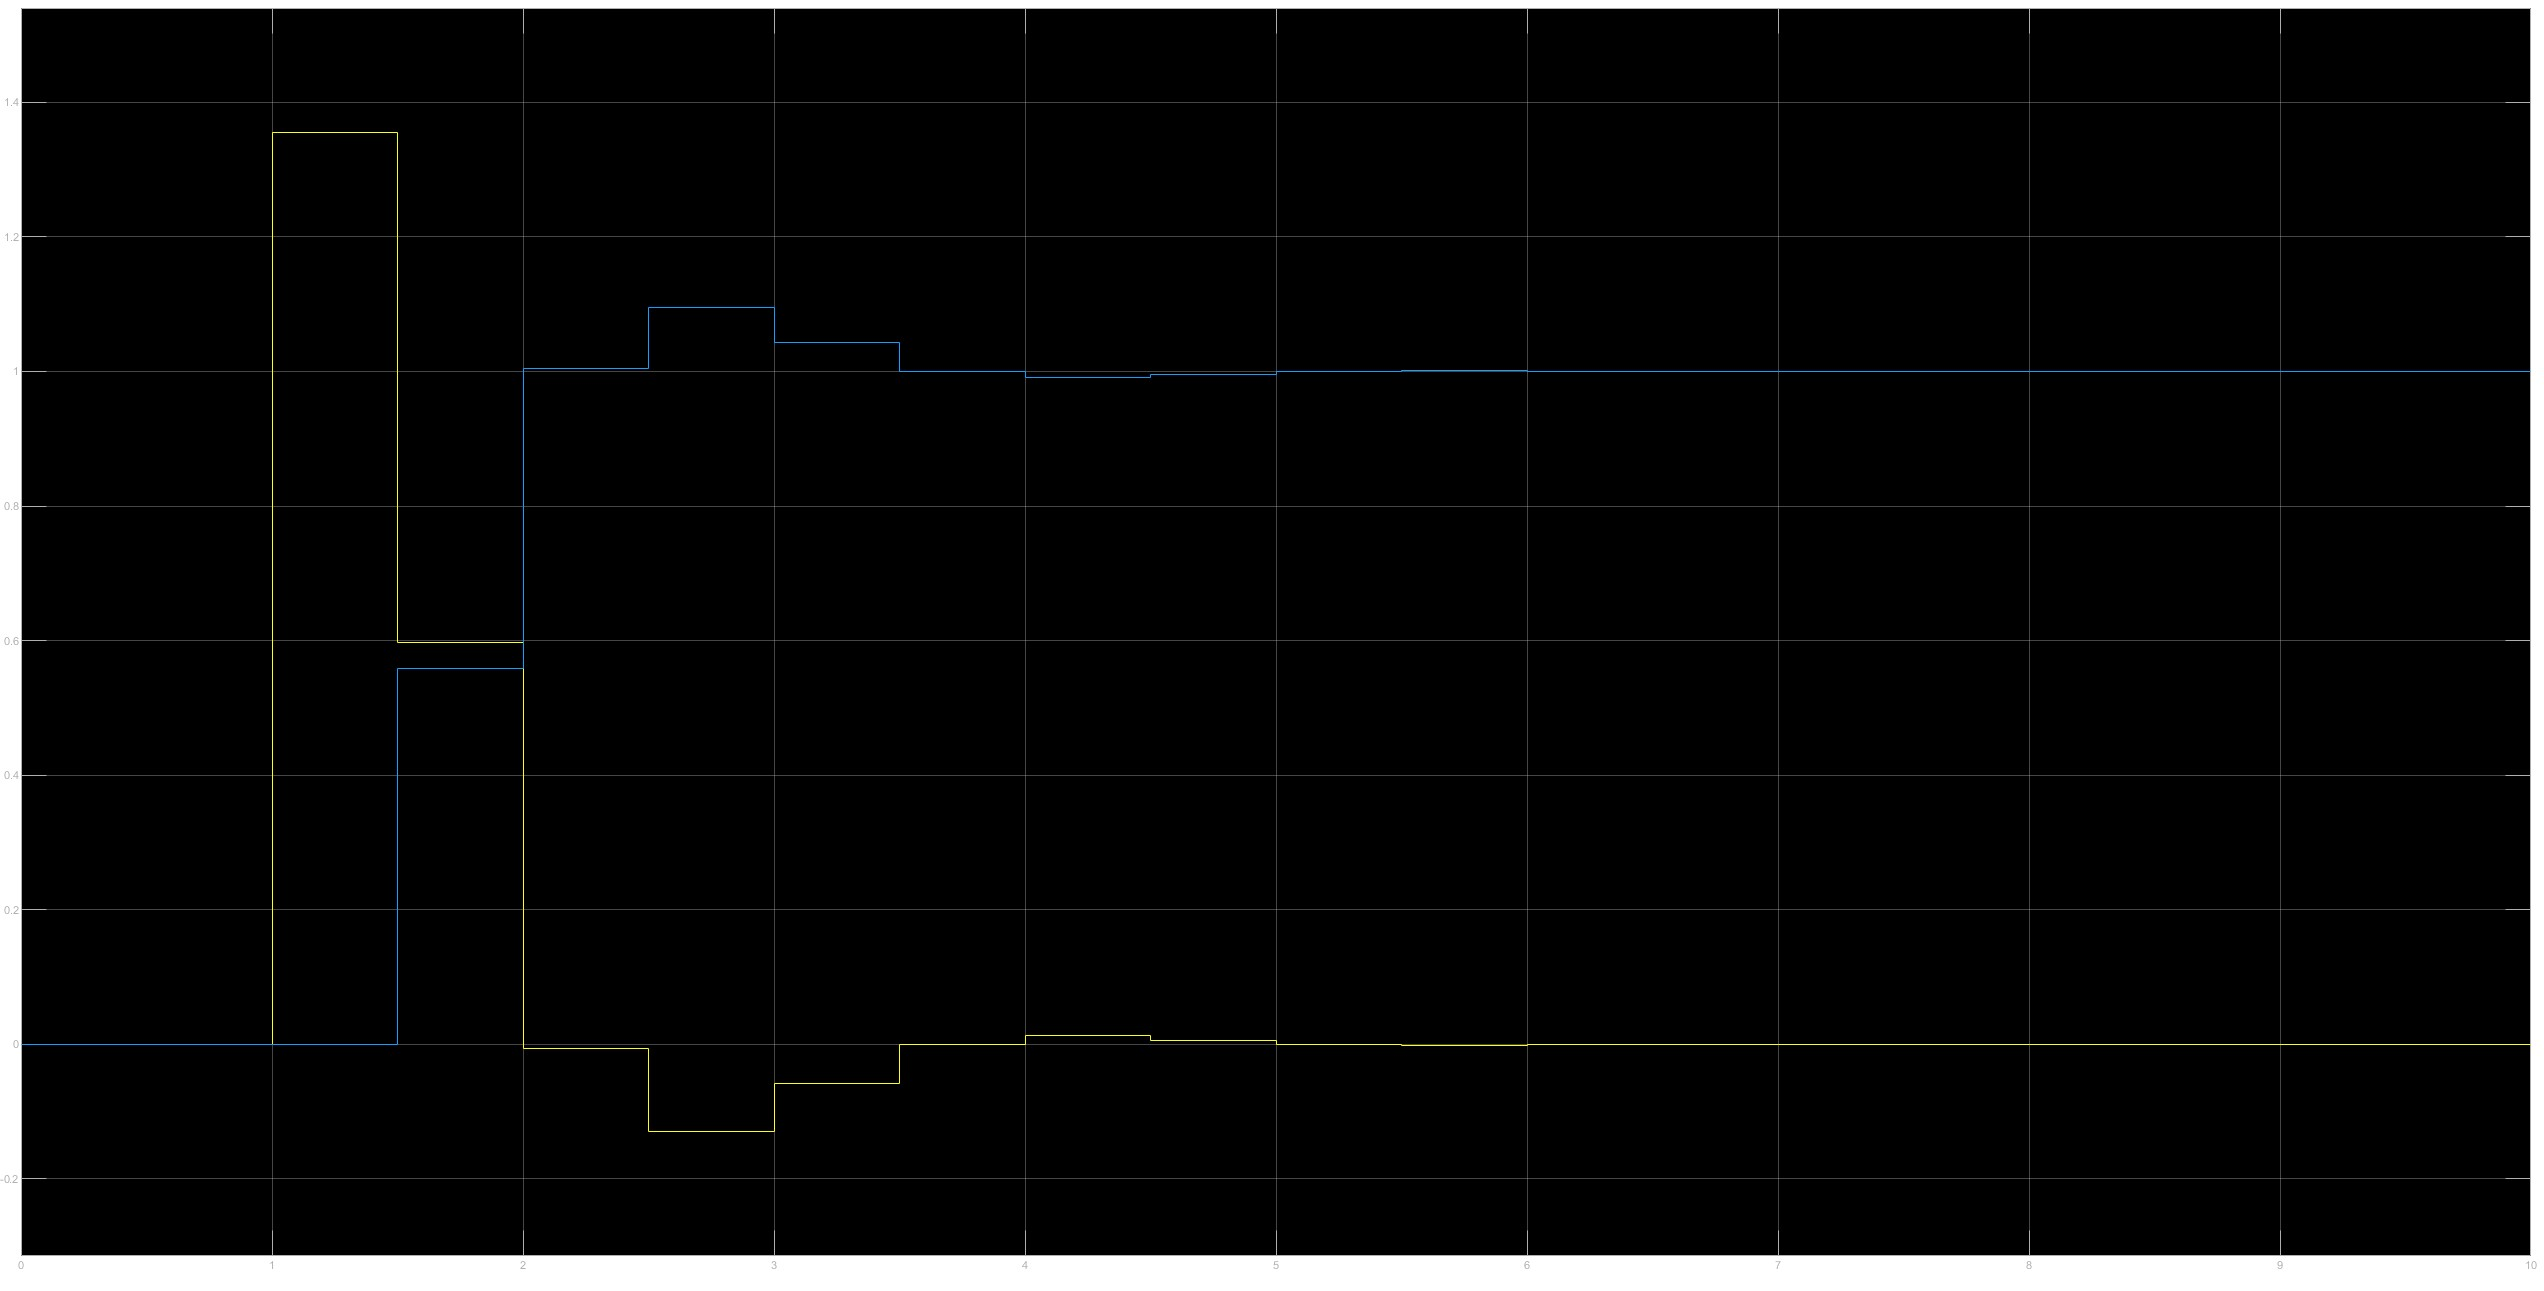
\includegraphics[width=1.1\textwidth]{pictures/task2_0.5_step_response_1.jpg}
\end{figure}
\begin{figure}[H]
    \caption{$T_s = 0.5$: Step Response when the gain is 0.7494}
    \label{fig:0.5_Ts_step_response_2}
    \centering
    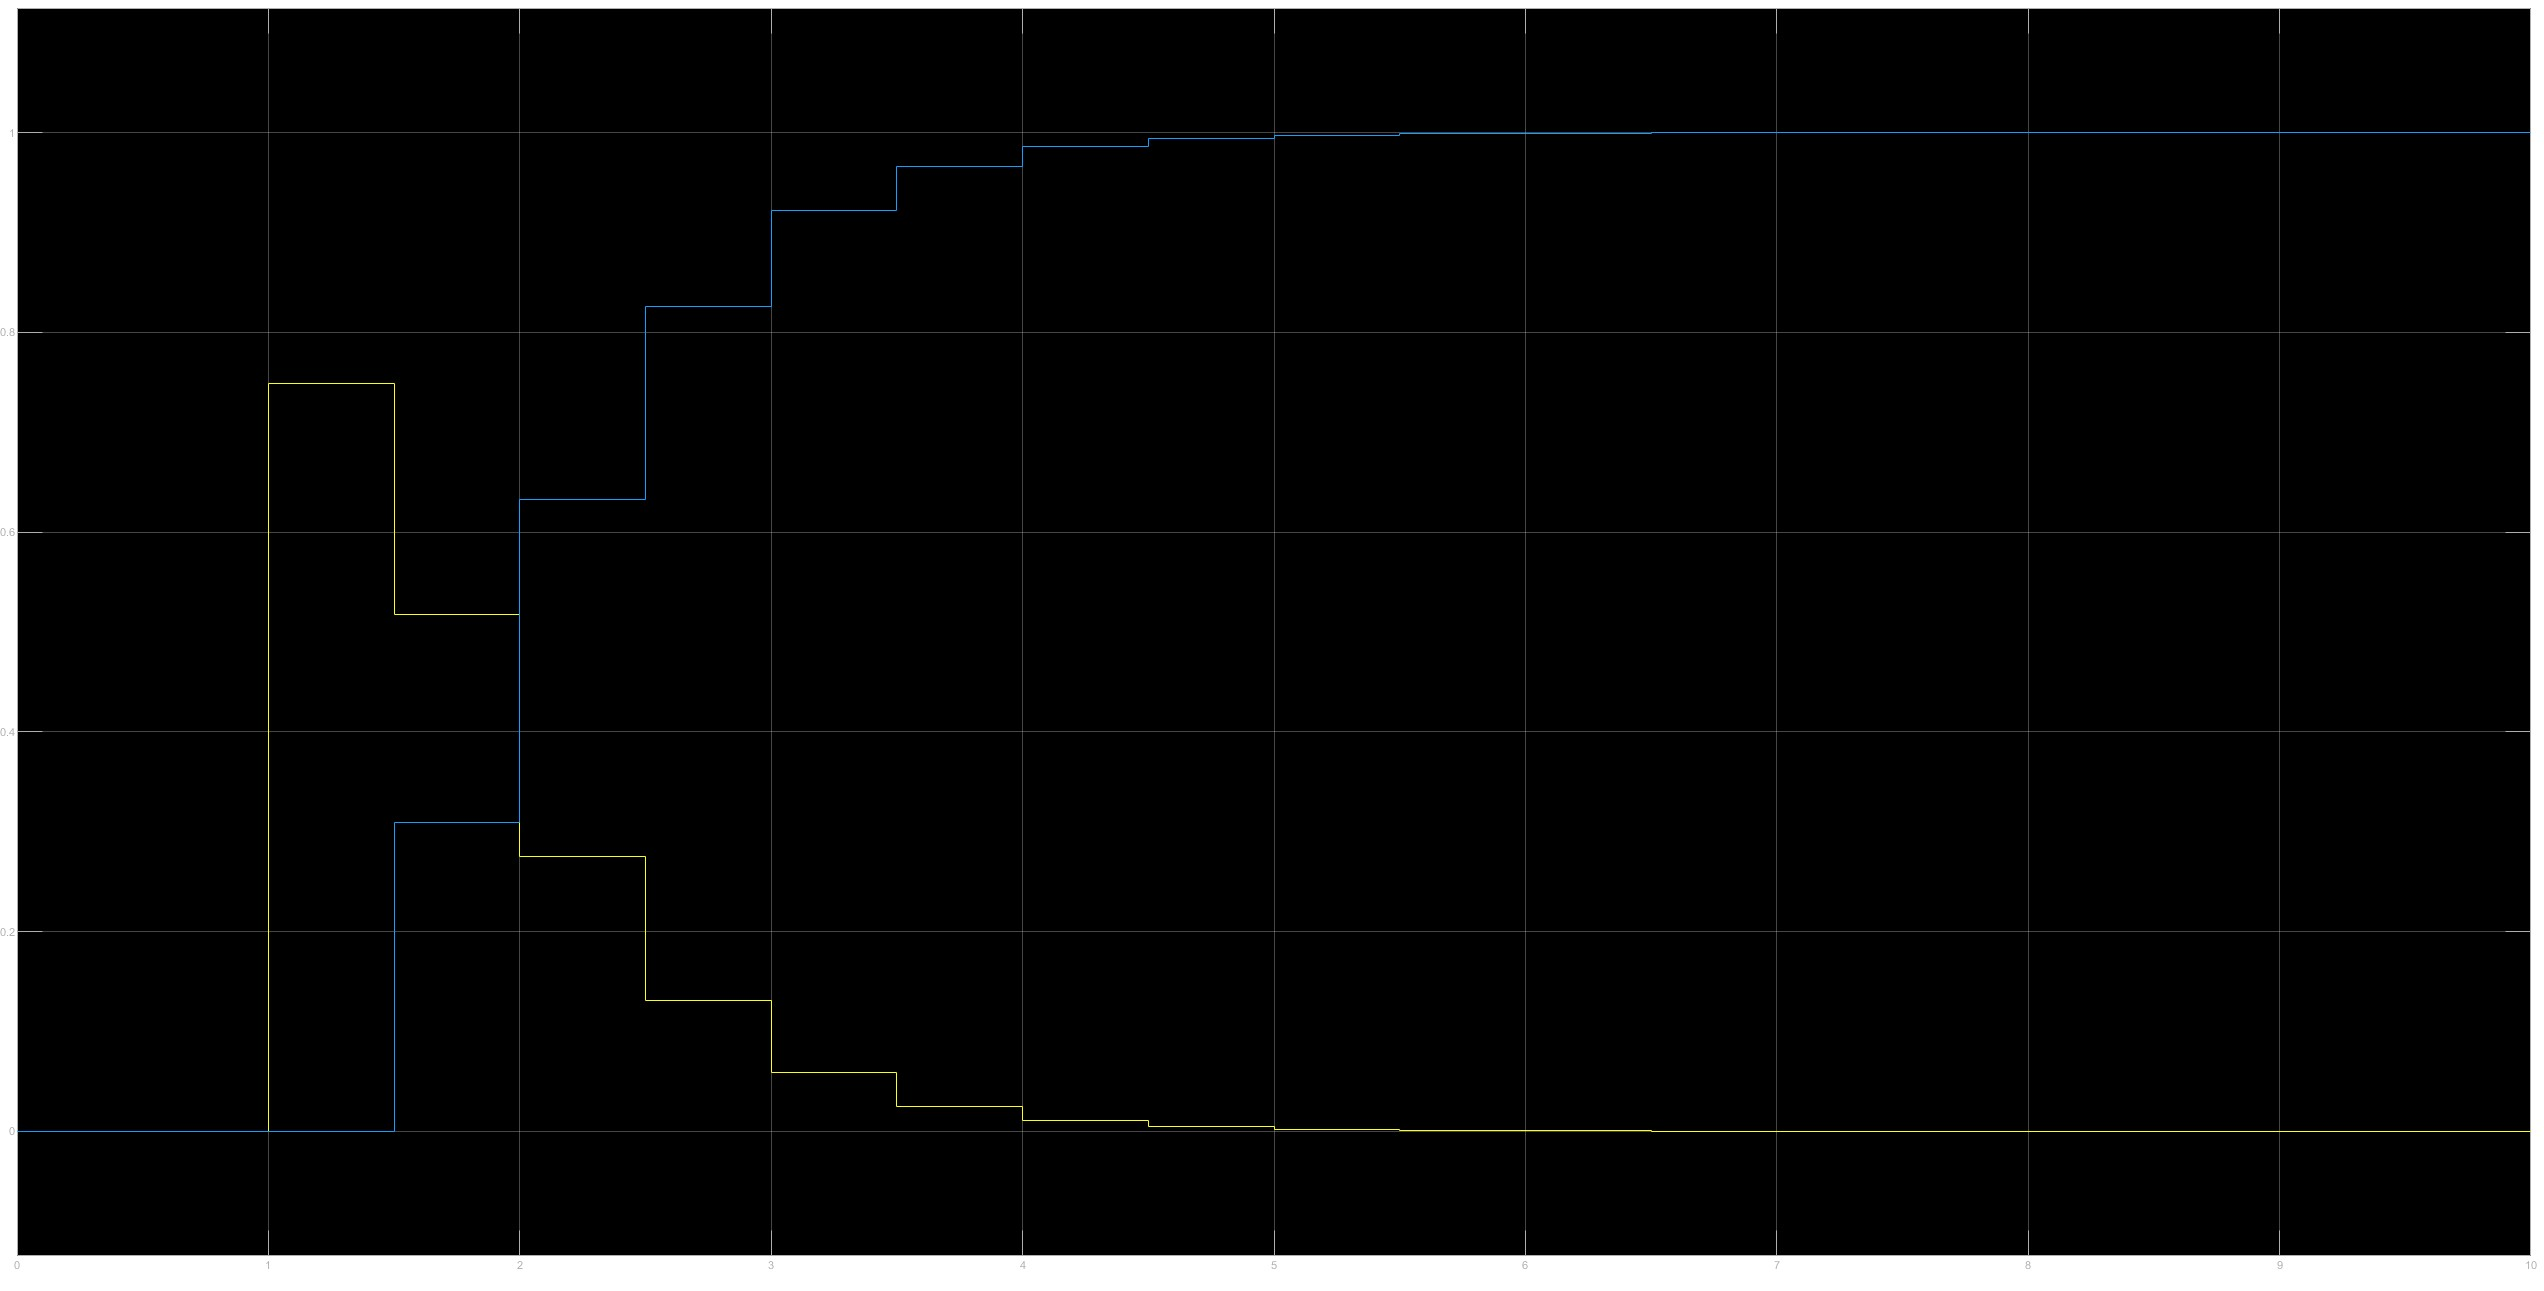
\includegraphics[width=1.1\textwidth]{pictures/task2_0.5_step_response_2.jpg}
\end{figure}
\begin{figure}[H]
    \caption{$T_s = 1.0$: Step Response when the gain is 0.8609}
    \label{fig:1.0_Ts_step_response_2}
    \centering
    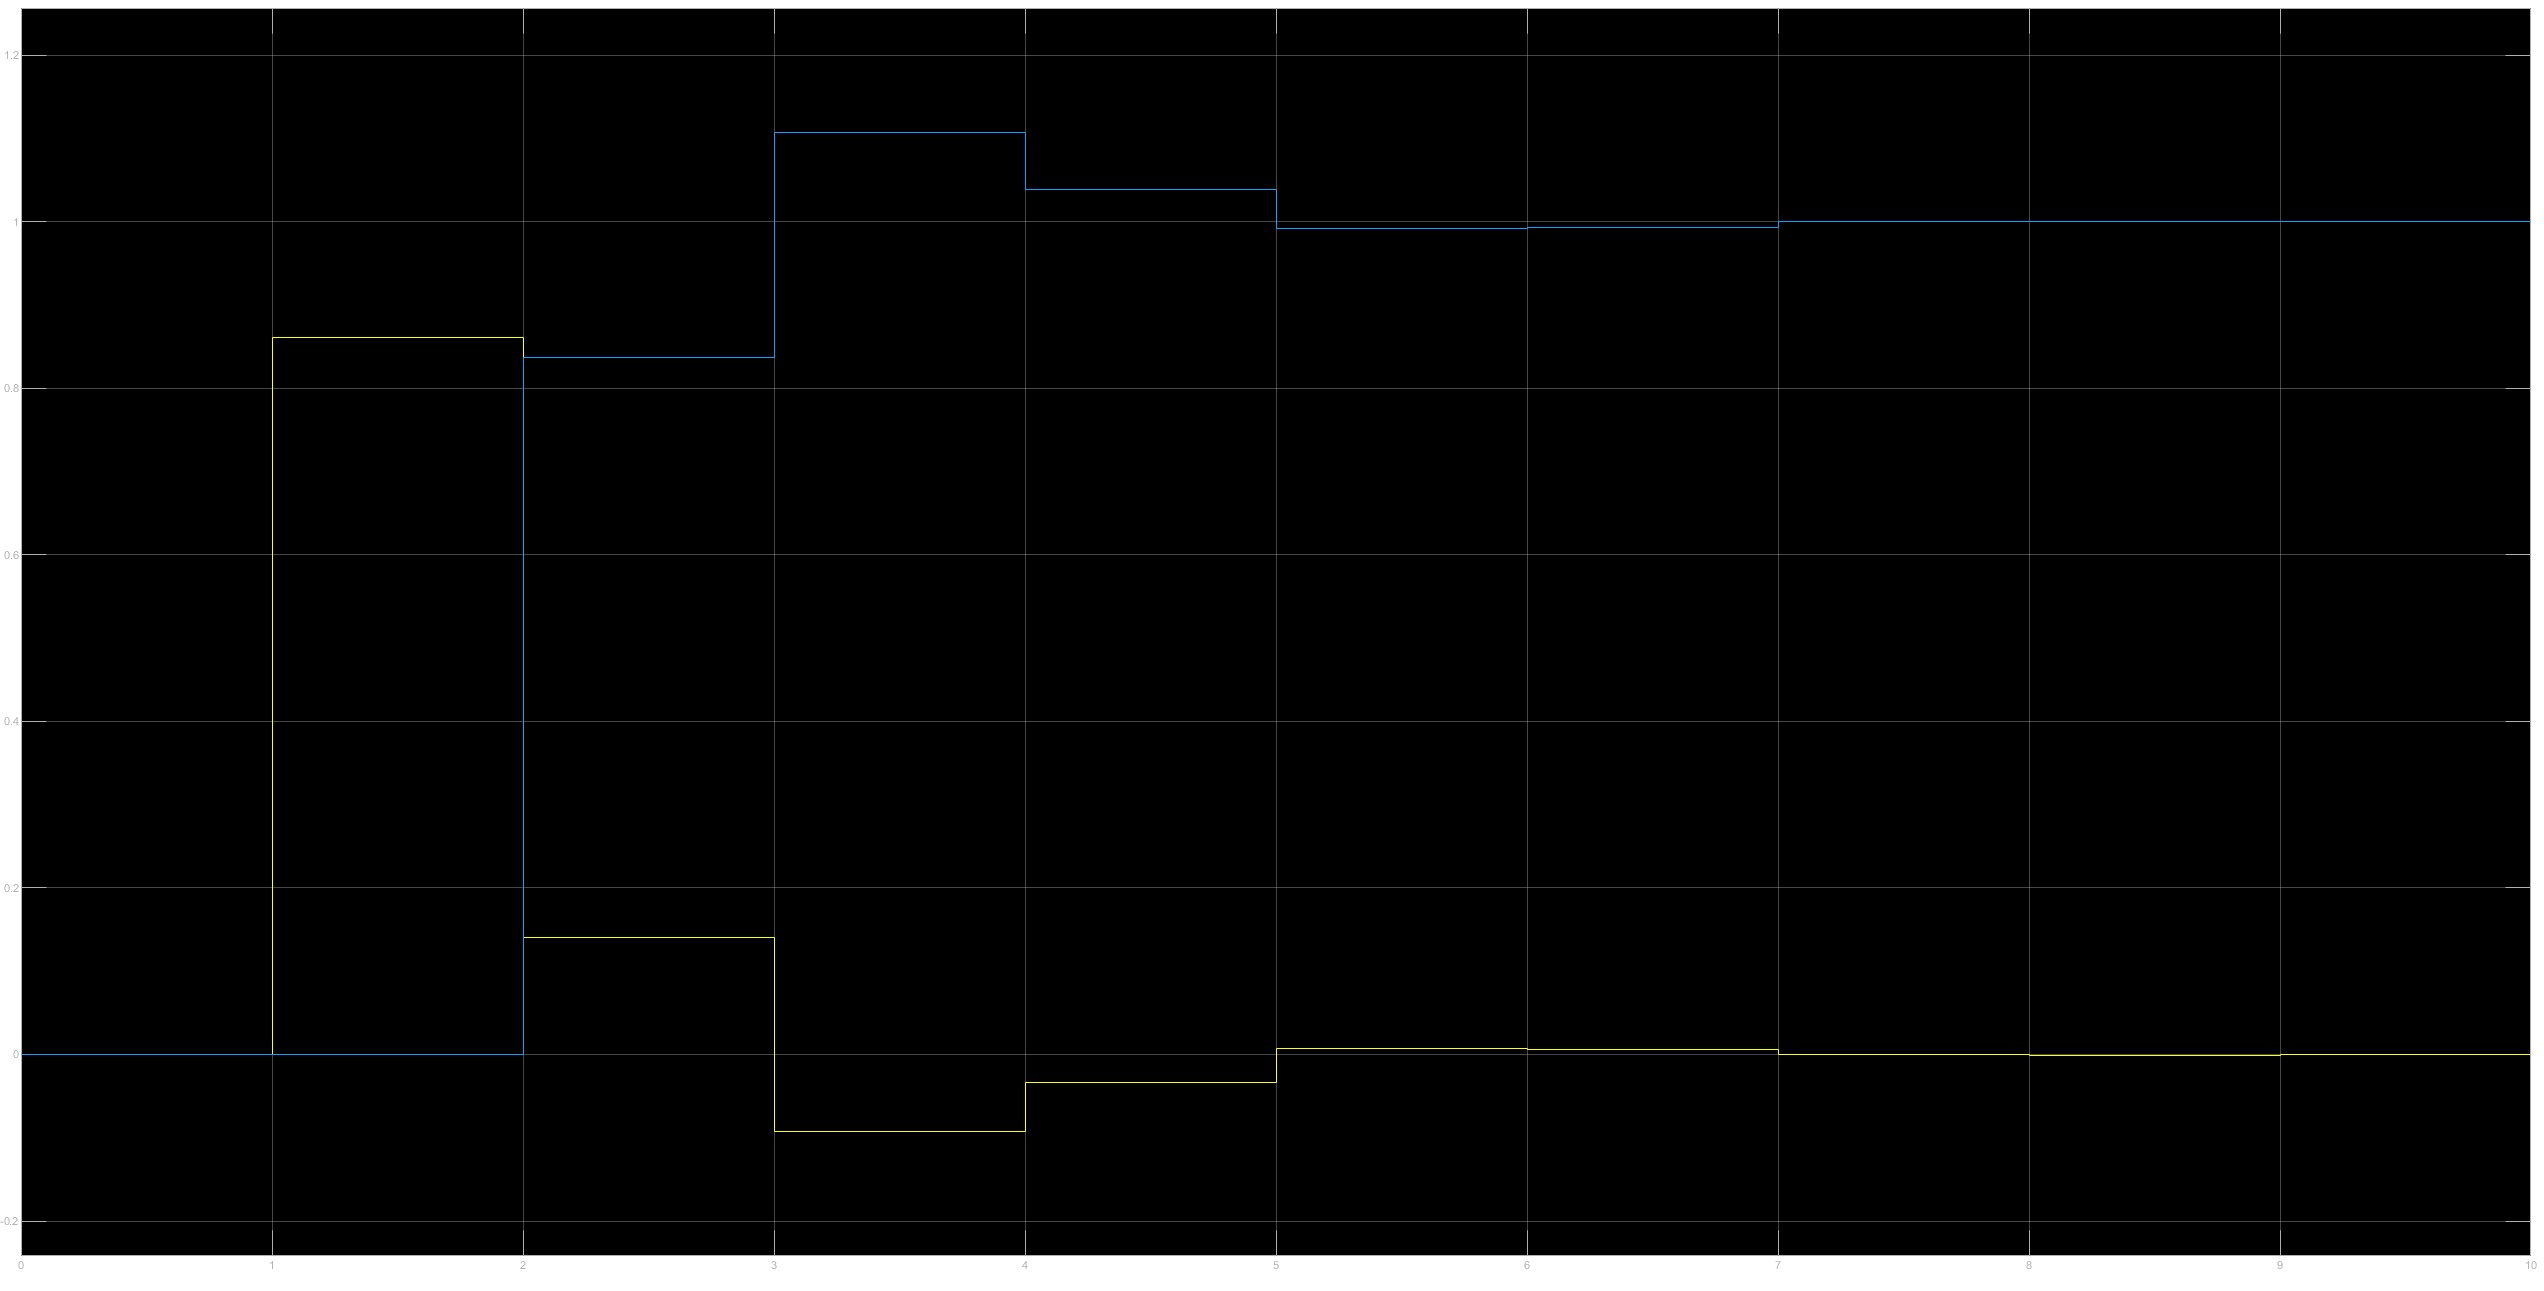
\includegraphics[width=1.1\textwidth]{pictures/task2_1.0_step_response_1.jpg}
\end{figure}
\begin{figure}[H]
    \caption{$T_s = 1.0$: Step Response when the gain is 0.4715}
    \label{fig:1.0_Ts_step_response_2}
    \centering
    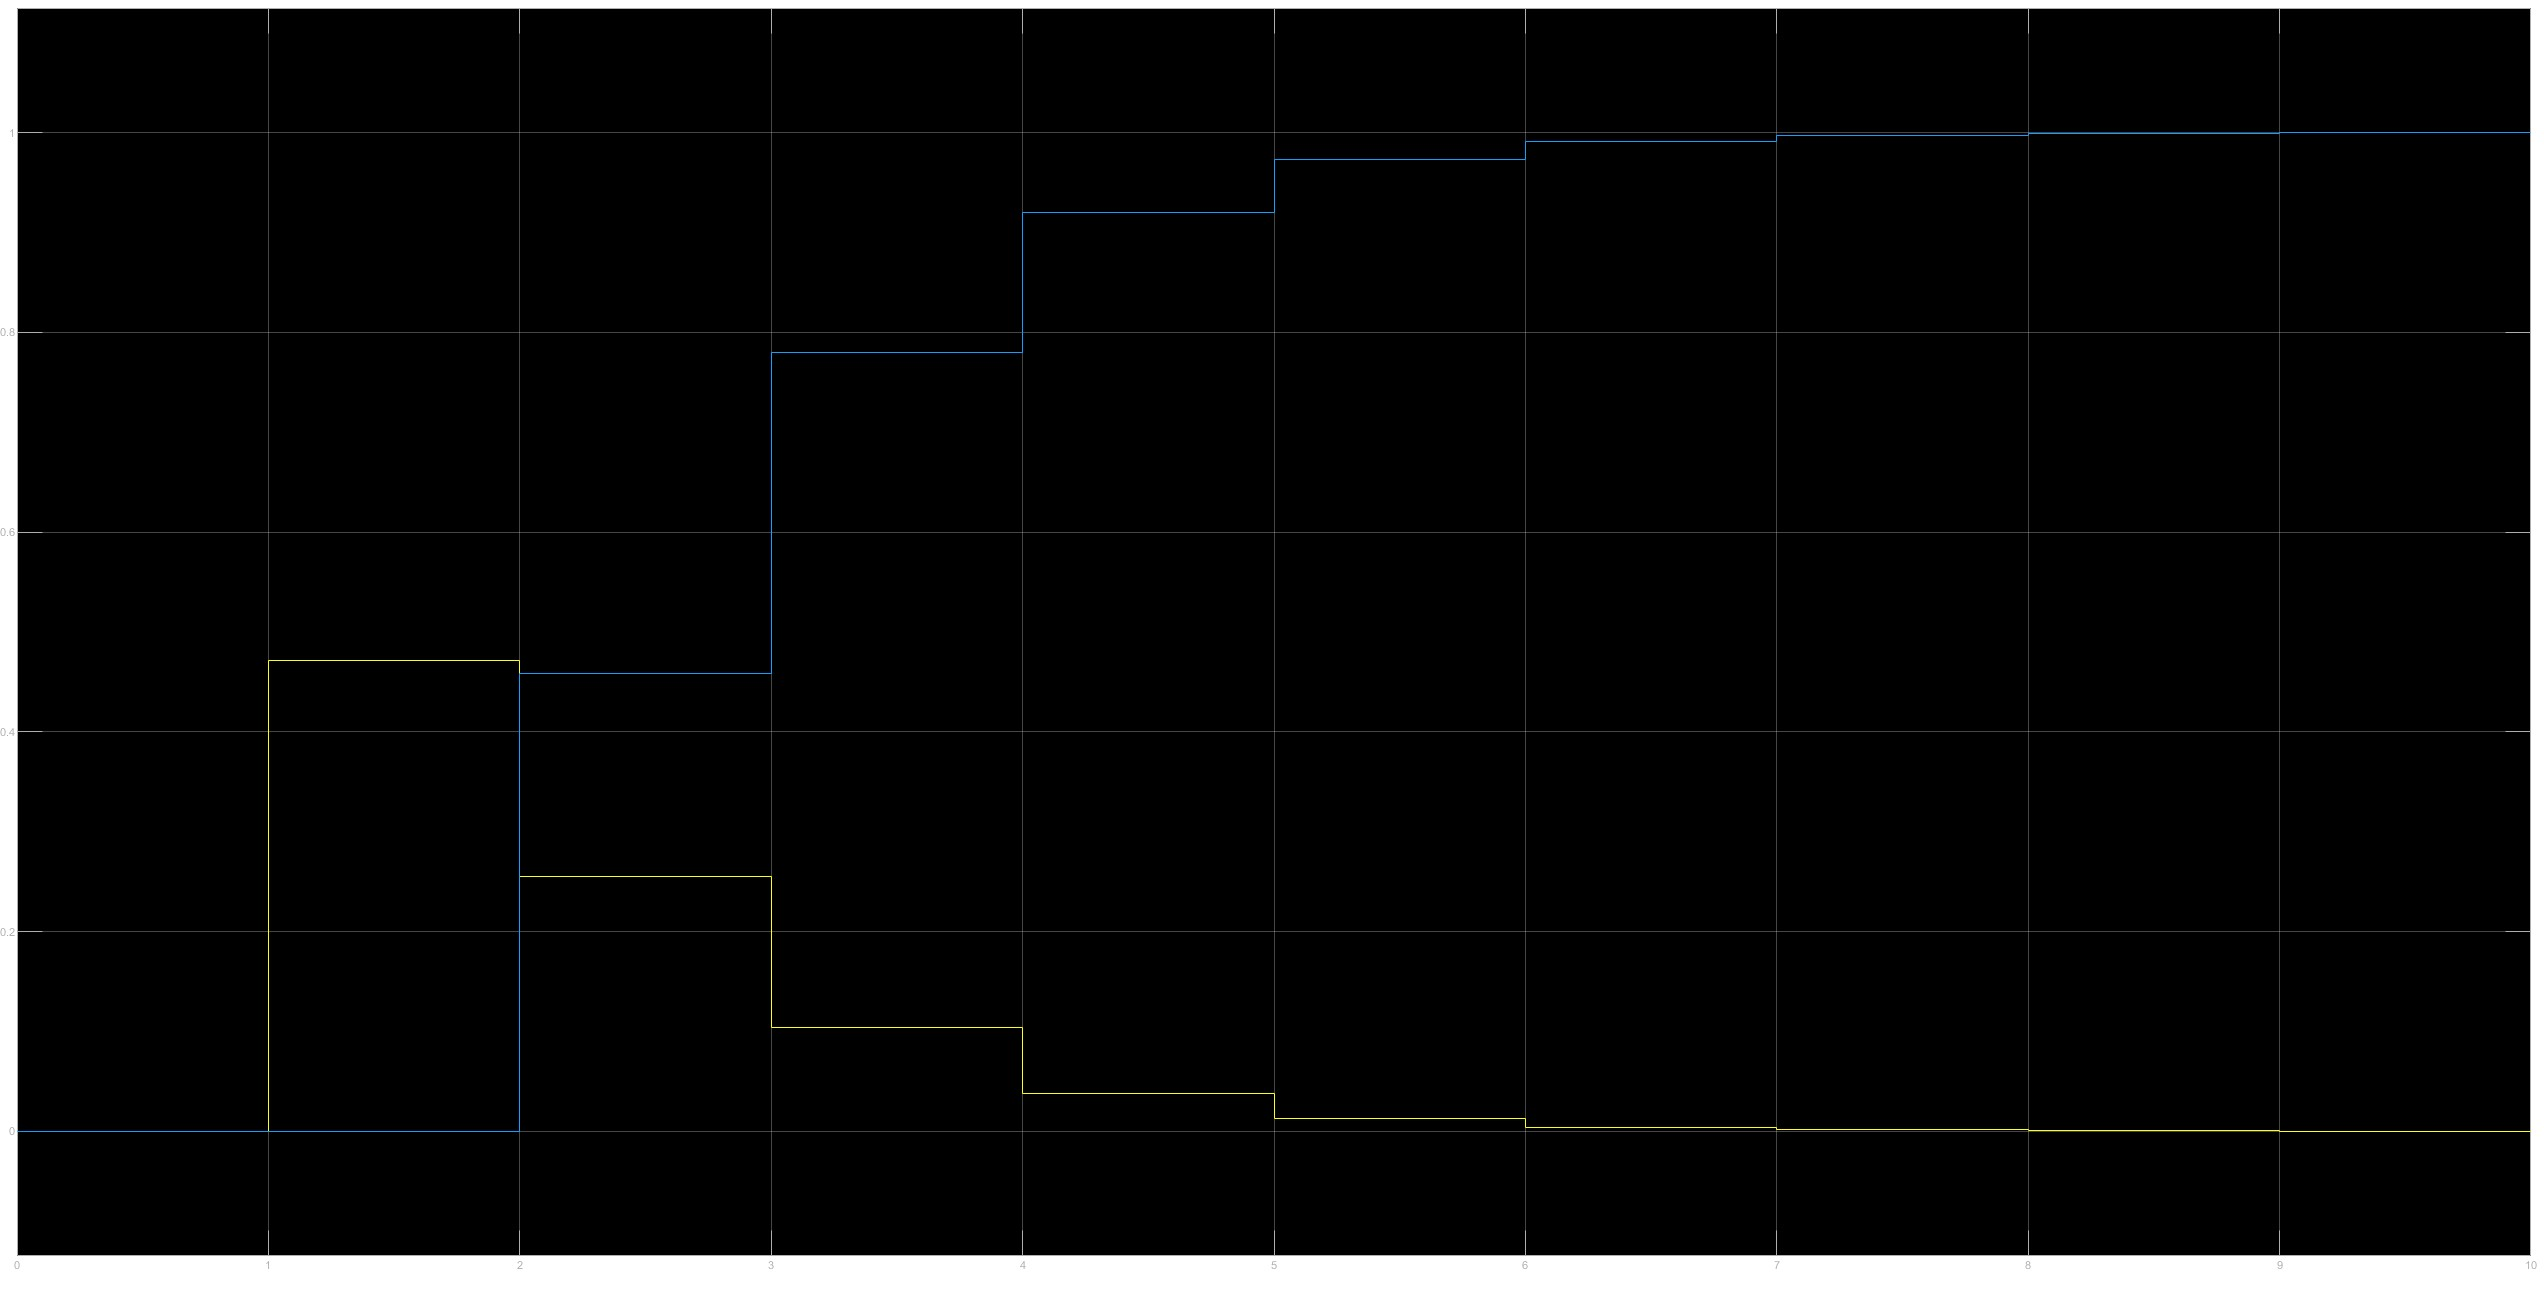
\includegraphics[width=1.1\textwidth]{pictures/task2_1.0_step_response_2.jpg}
\end{figure}
\subsubsection{Step 3}
In step 3, the DC Servo's control is simulated using both Proportional and Derivative digital control for two different sampling times; 0.01 and 0.1 seconds. Step 3 produces the same set of results as step 2. Table 1.2 displays the values of $K_p$, $K_d$ and the transfer function $G_{ol}$ for the different settling times. Damping ratio ($\zeta$) remains constant at a value of 1 throughout. 
\begin{table}[]
    \centering
    \caption{The values of Proportional Gain $K_p$ and Derivative Gain $K_d$ with the transfer function they produce $G_{ol}$. }
    \label{tab:task2_gain_table}
    \begin{tabular}{@{}cccc@{}}
    \toprule
    \textbf{Sampling Time} & \textbf{Proportional Gain} & \textbf{Derivative Gain} & \textbf{Transfer Function}                                                          \\ \midrule
    \textbf{$T_s$}         & $K_p$                      & $K_d$                    & $G_{ol}$                                                                            \\
    0.01                   & 5.7654                     & 0.1441                   & ${{1.398e-05 z^2 + 3.66e-06 z - 9.746e-06}\over{0.01 z^3 - 0.0193 z^2 + 0.0093 z}}$ \\
    0.1                    & 3.6316                     & 0.0908                   & ${{0.004072 z^2 + 0.002386 z - 0.0006401}\over{0.1 z^3 - 0.1484 z^2 + 0.0484 z}}$  
    \end{tabular}
\end{table}
The root locus plots for sampling times of 0.01 and 0.1 can be found below in Figures 1.18 and 1.19.
\begin{figure}[H]
    \caption{$T_s = 0.01$: Root Locus Plot of Derivative and Proportional Control}
    \label{fig:0.01_Ts_step3_root_locus}
    \centering
    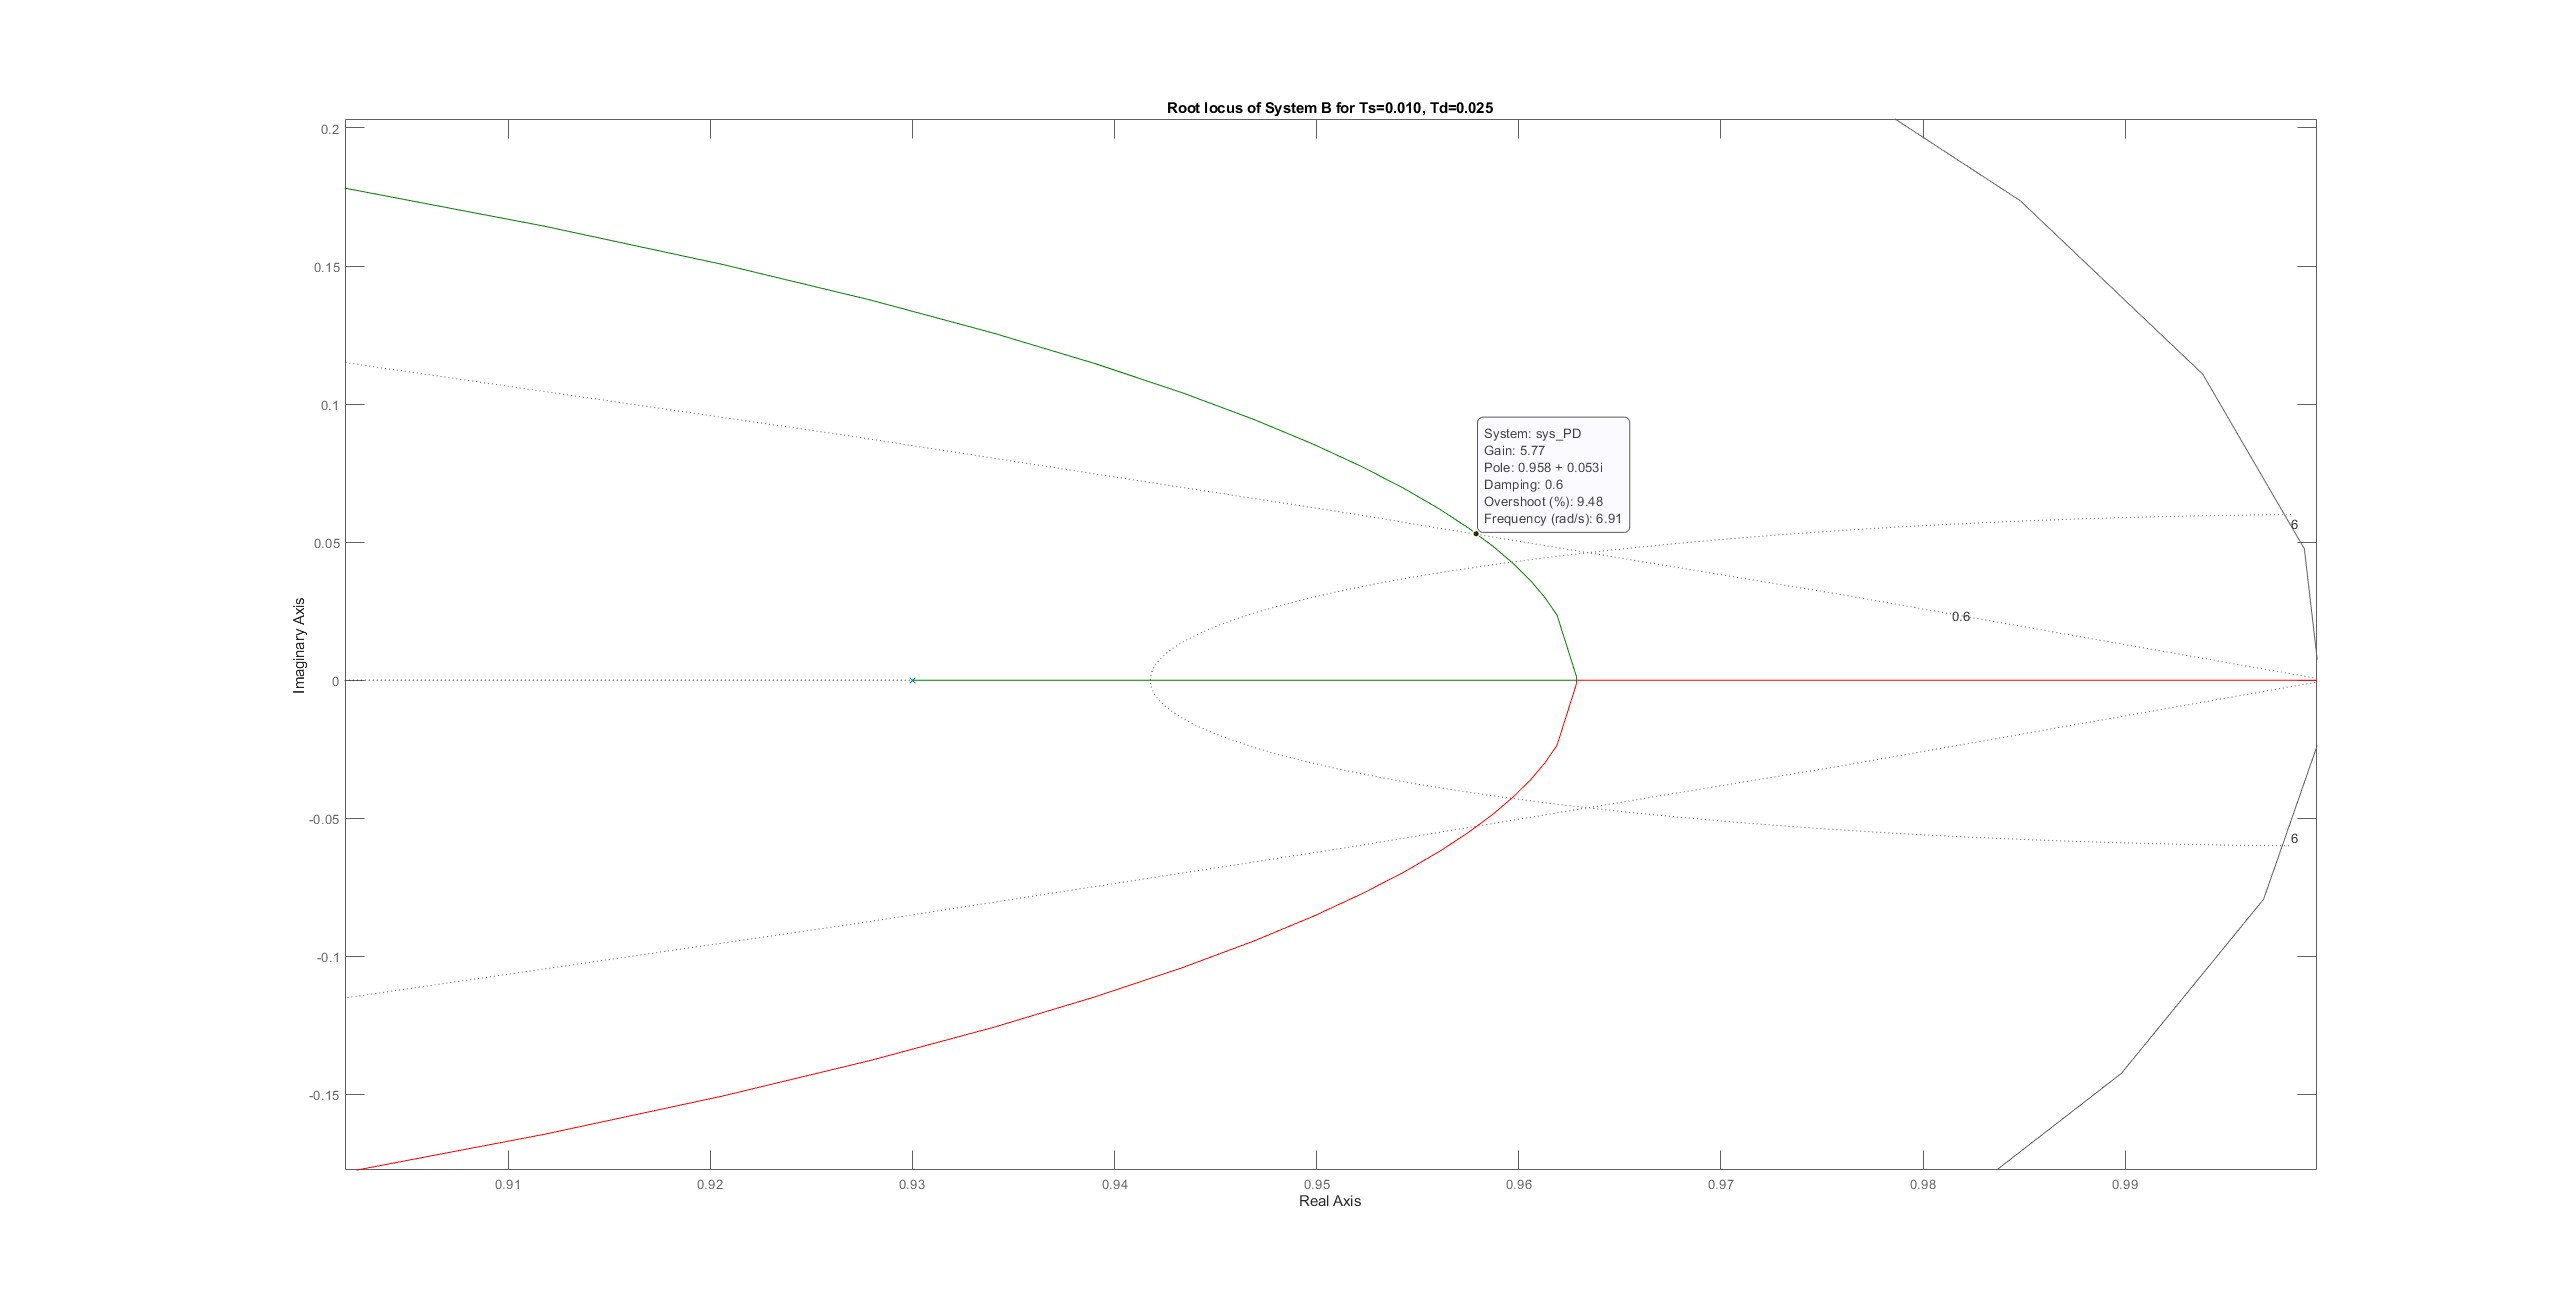
\includegraphics[width=1.1\textwidth]{pictures/task3_0.01.jpg}
\end{figure}
\begin{figure}[H]
    \caption{$T_s = 0.1$: Root Locus Plot of Derivative and Proportional Control}
    \label{fig:0.1_Ts_step3_root_locus}
    \centering
    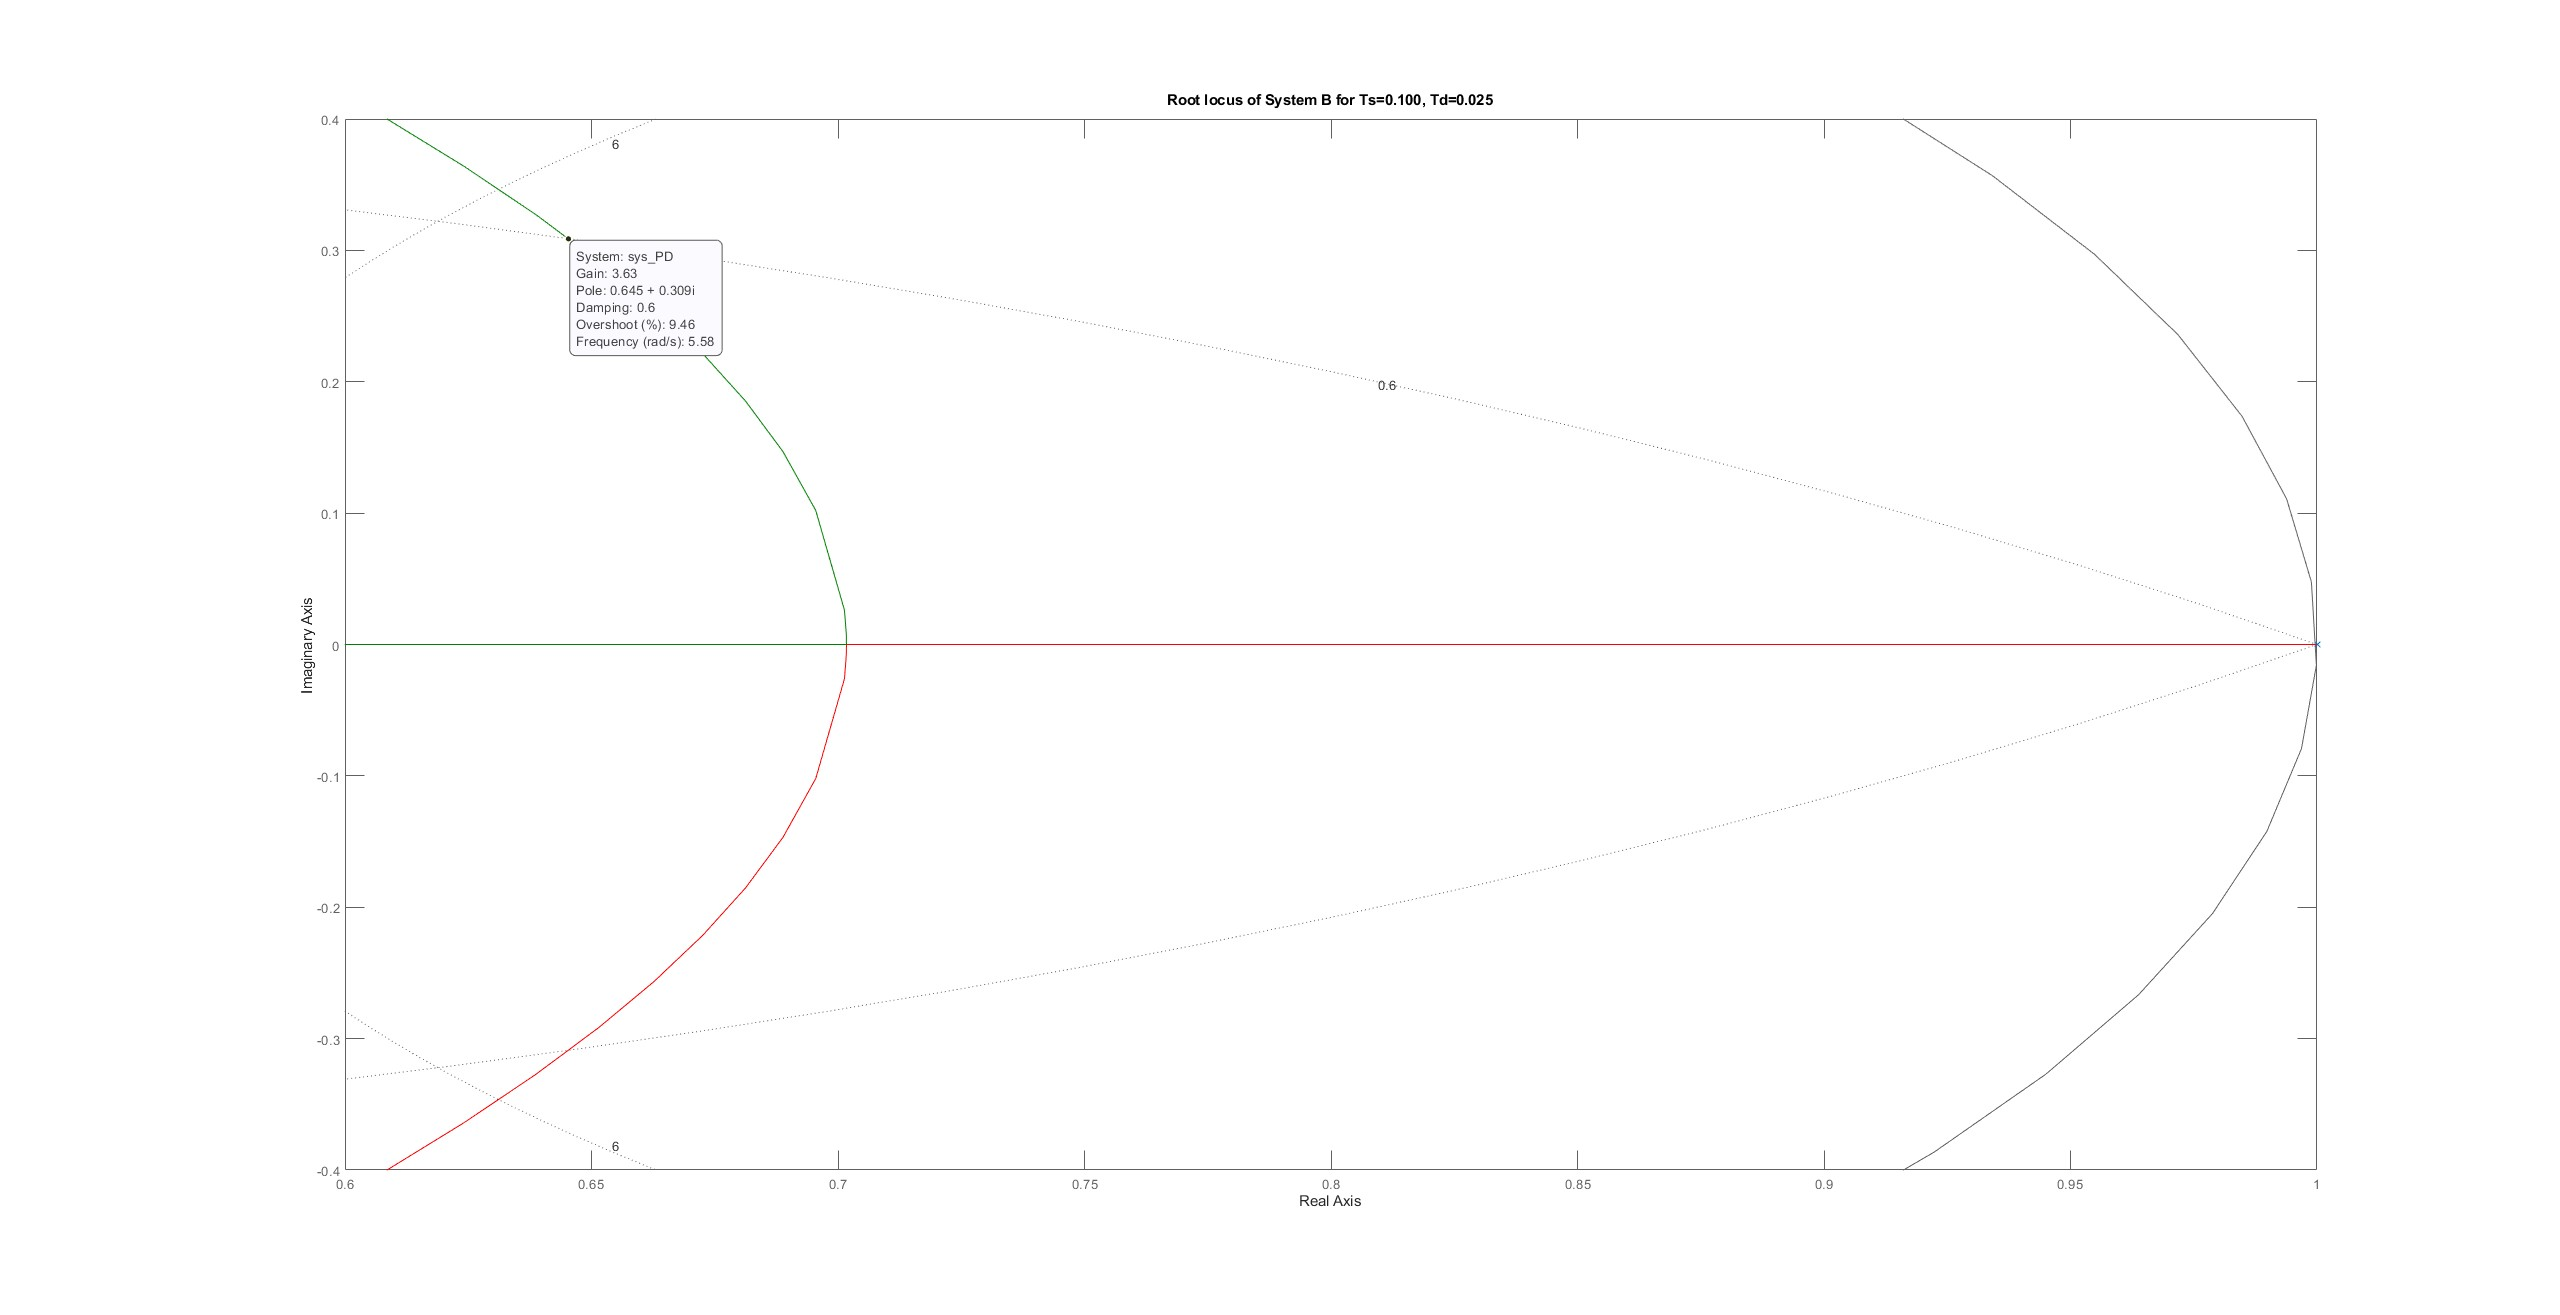
\includegraphics[width=1.1\textwidth]{pictures/task3_0.1.jpg}
\end{figure}
Finally the step response plots of the simulation can be plotted for settling times of 0.01 and 0.1 seconds. They are found in Figures 1.20 and 1.21 respectively.
\begin{figure}[H]
    \caption{$T_s = 0.01$: Step Response of Derivative and Proportional Control}
    \label{fig:0.01_Ts_step3_step_response}
    \centering
    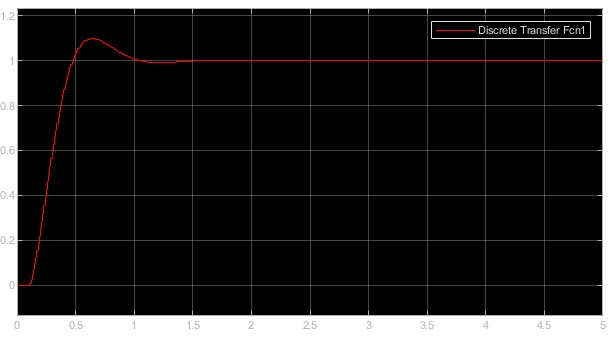
\includegraphics[width=1.1\textwidth]{pictures/task3_0.01_step_response.jpg}
\end{figure}
Figure 1.20 shows an overdamped response. It can be categorised as such because of the high maximum overshoot of the response and the small oscillation that occurs to return to its original value.
\begin{figure}[H]
    \caption{$T_s = 0.1$: Step Response of Derivative and Proportional Control}
    \label{fig:0.1_Ts_step3_step_response}
    \centering
    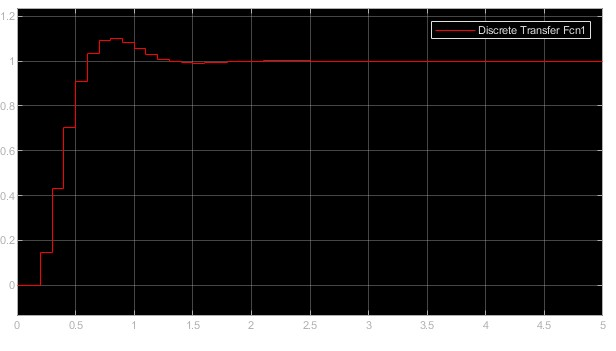
\includegraphics[width=1.1\textwidth]{pictures/task3_0.1_step_response.jpg}
\end{figure}
Figure 1.21 behaves in a similar fashion to the response in Figure 1.21. However, this response is more "blocky", which is due to the increased sampling time for this simulation.
\subsubsection{Step 4}
In step 4, the values of gains $K_p$ and $K_d$ obtained in the previous two steps were taken, and tuned into the real DC Servo rig, to produce step responses. The following eight figures (1.22 to 1.29) show the responses of the DC Servo when using only Digital-Proportional control. 
\begin{figure}[H]
    \caption{$T_s = 0.01$, $K_p = 4.2518$: Step Response of Proportional Control - Real DC Servo Rig}
    \label{fig:0.01_Ts_step4_step_response_1}
    \centering
    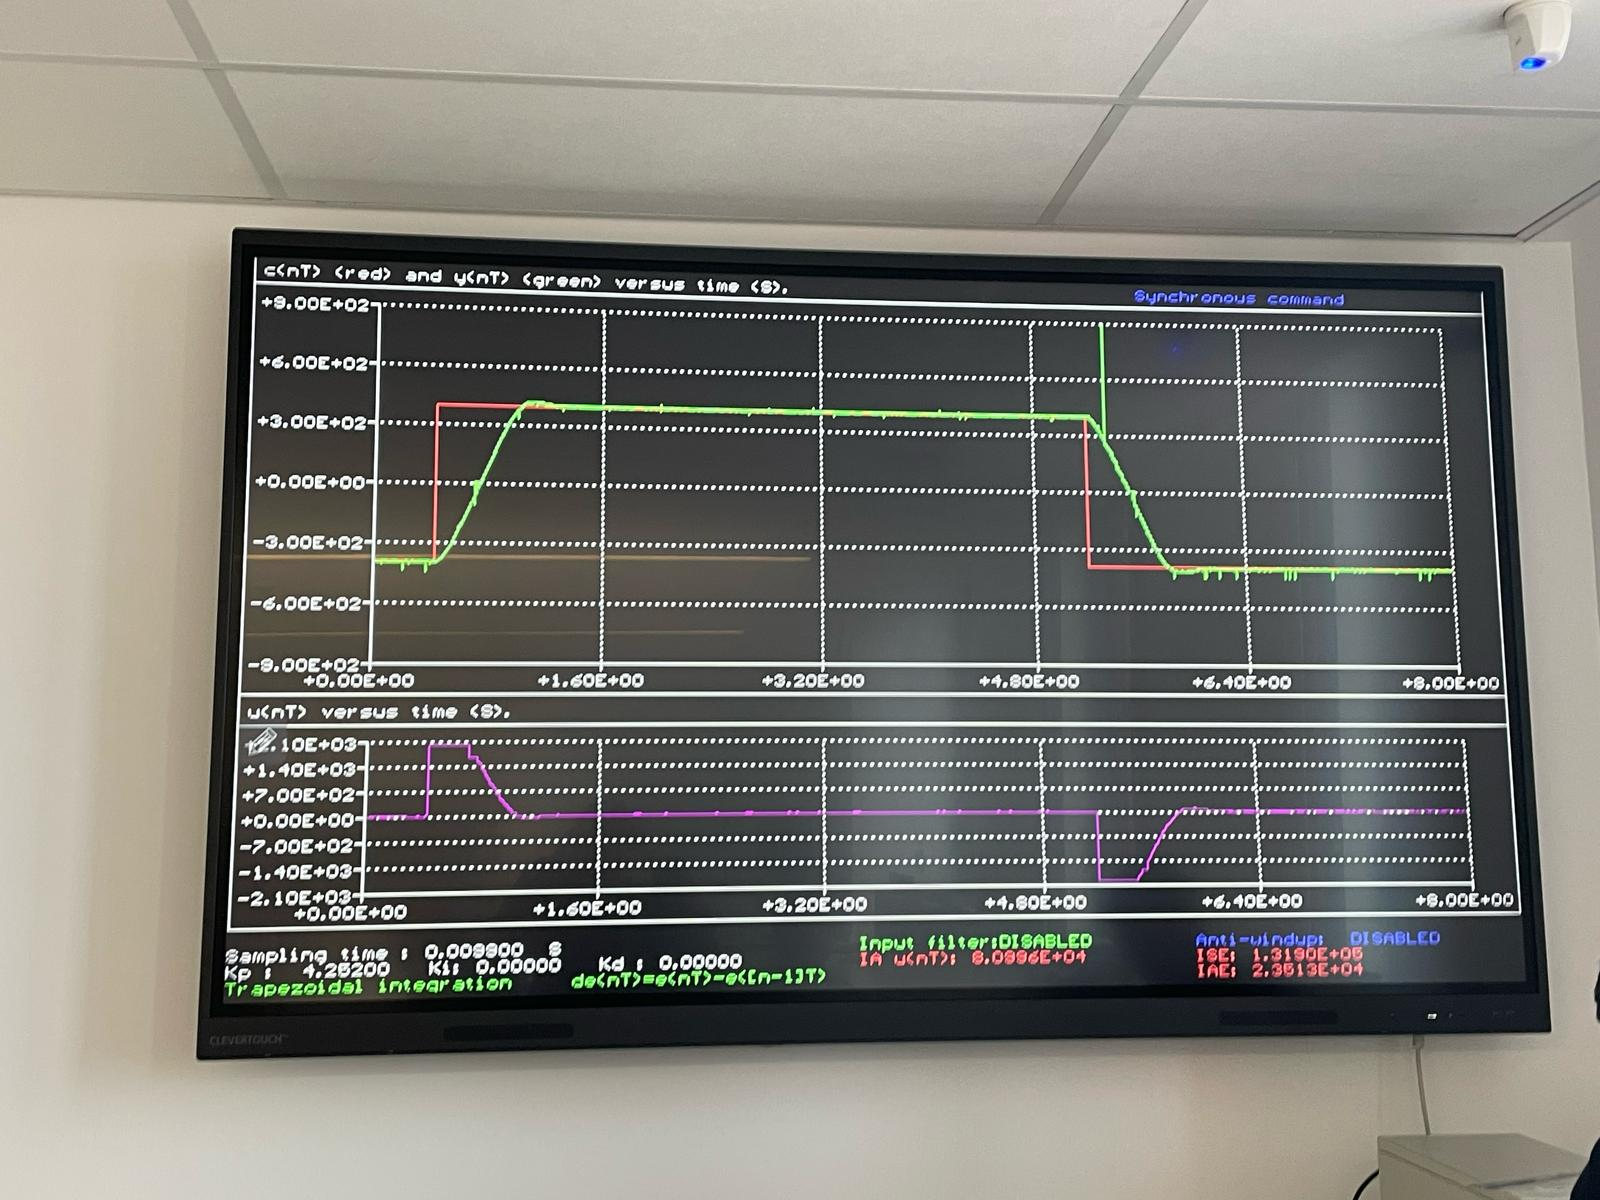
\includegraphics[width=1.1\textwidth]{pictures/task4_kp_0.01_1}
\end{figure}
Figure 1.22 shows a response that is almost critically damped, with a very slight overshoot when returning to the original value.
\begin{figure}[H]
    \caption{$T_s = 0.01$, $K_p = 1.5801$: Step Response of Proportional Control - Real DC Servo Rig}
    \label{fig:0.01_Ts_step4_step_response_2}
    \centering
    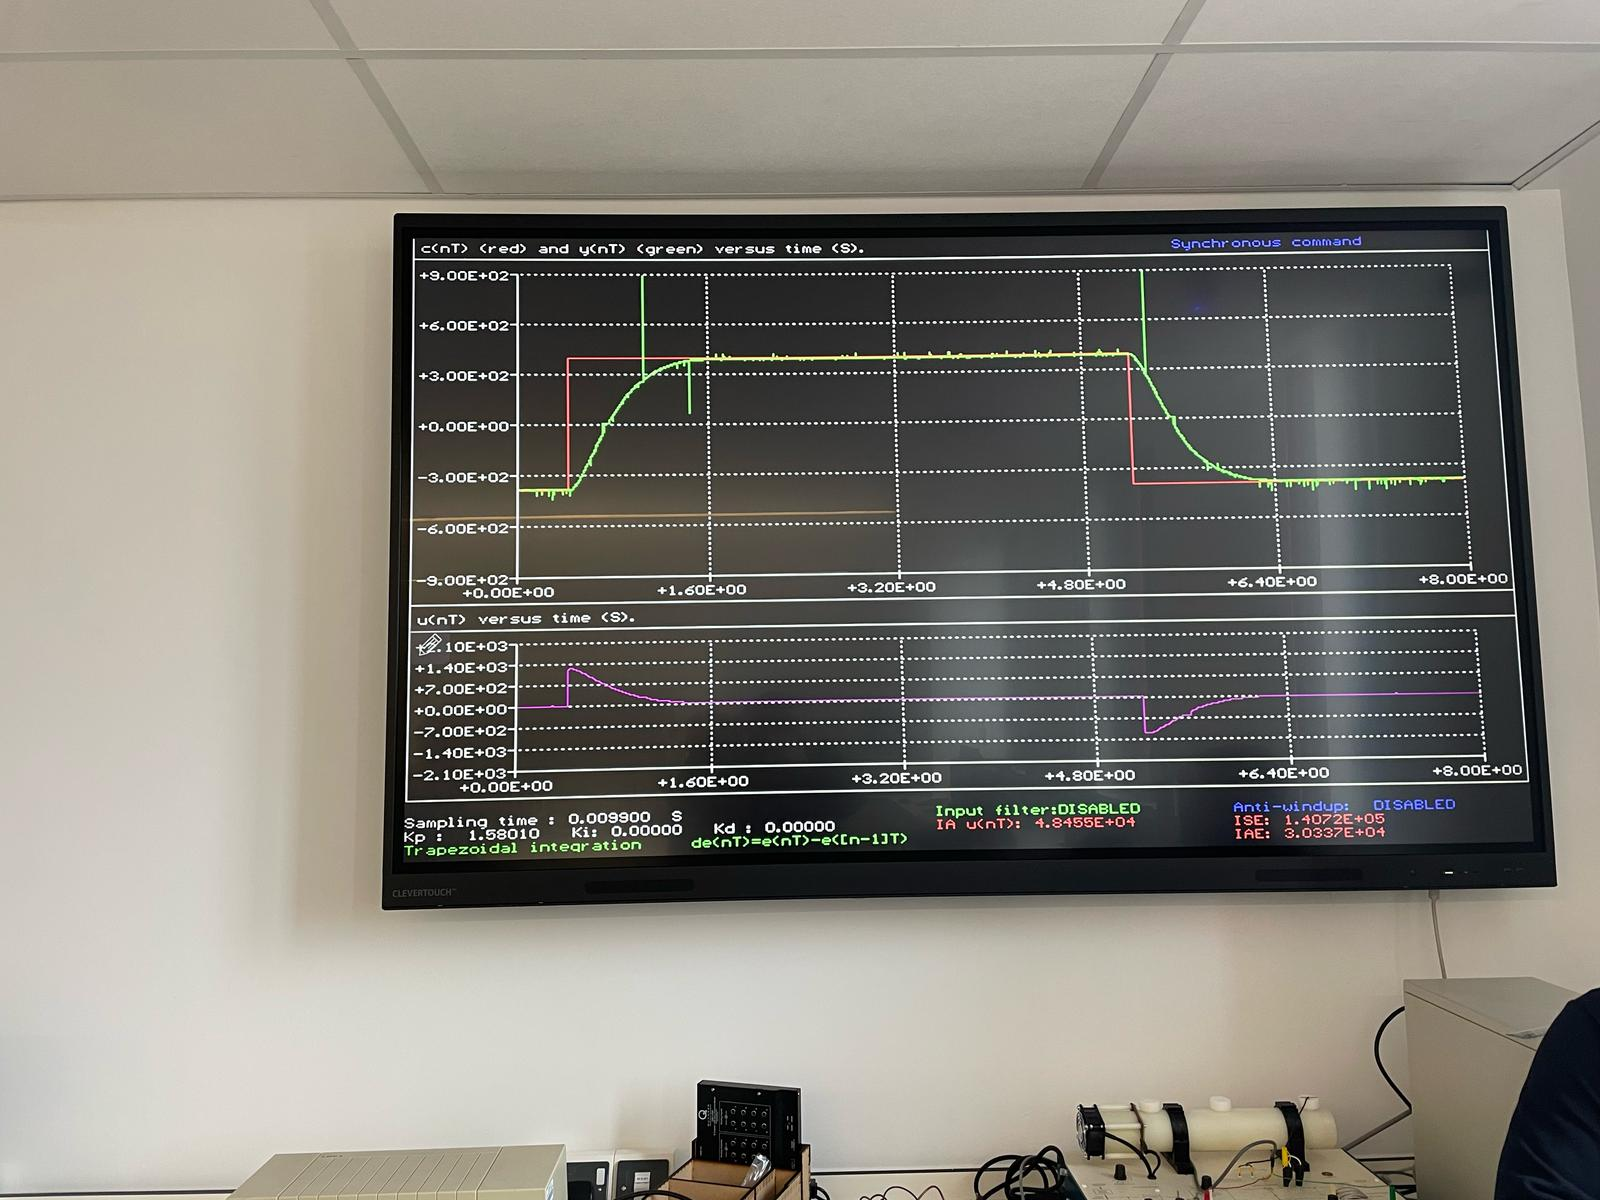
\includegraphics[width=1.1\textwidth]{pictures/task4_kp_0.01_2}
\end{figure}
Figure 1.23 shows a response that is critically damped, with no overshoot and a relatively small settling time.
\begin{figure}[H]
    \caption{$T_s = 0.1$, $K_p = 2.9833$: Step Response of Proportional Control - Real DC Servo Rig}
    \label{fig:0.1_Ts_step4_step_response_1}
    \centering
    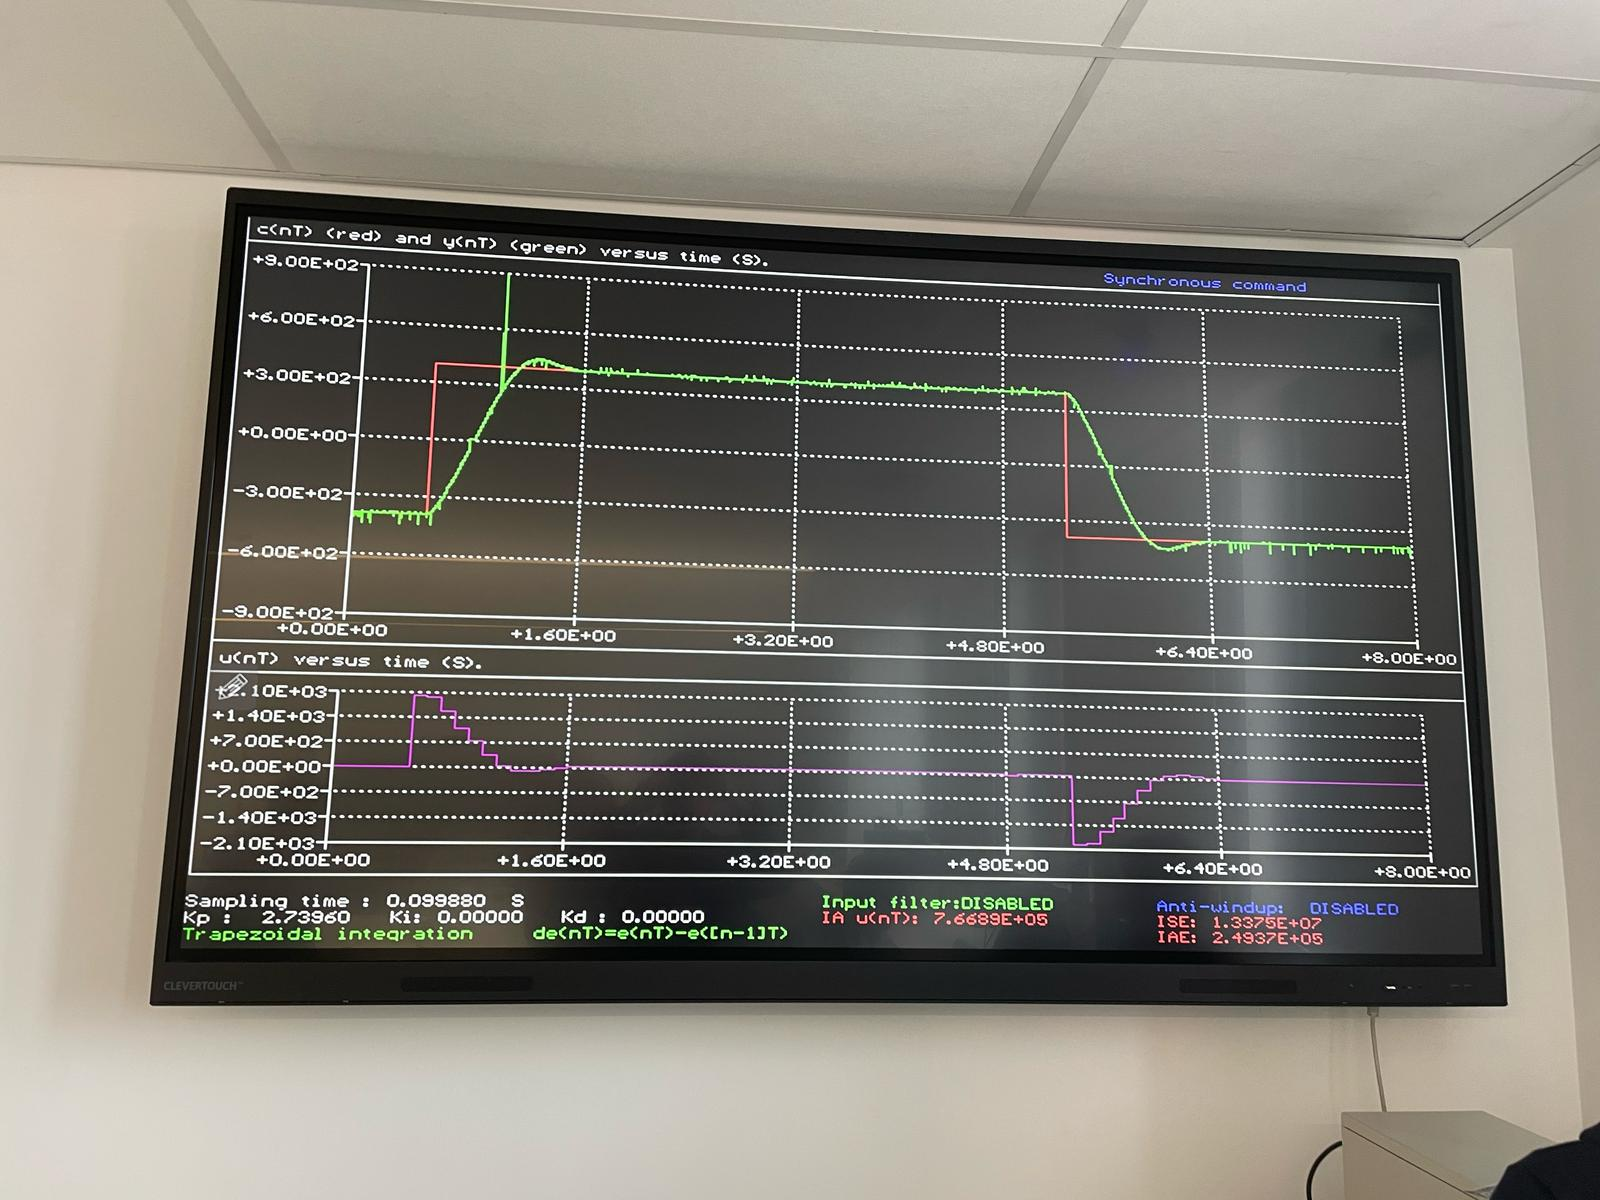
\includegraphics[width=1.1\textwidth]{pictures/task4_kp_0.1_1}
\end{figure}
Figure 1.24 shows an underdamped response. 
\begin{figure}[H]
    \caption{$T_s = 0.1$, $K_p = 1.3470$: Step Response of Proportional Control - Real DC Servo Rig}
    \label{fig:0.1_Ts_step4_step_response_2}
    \centering
    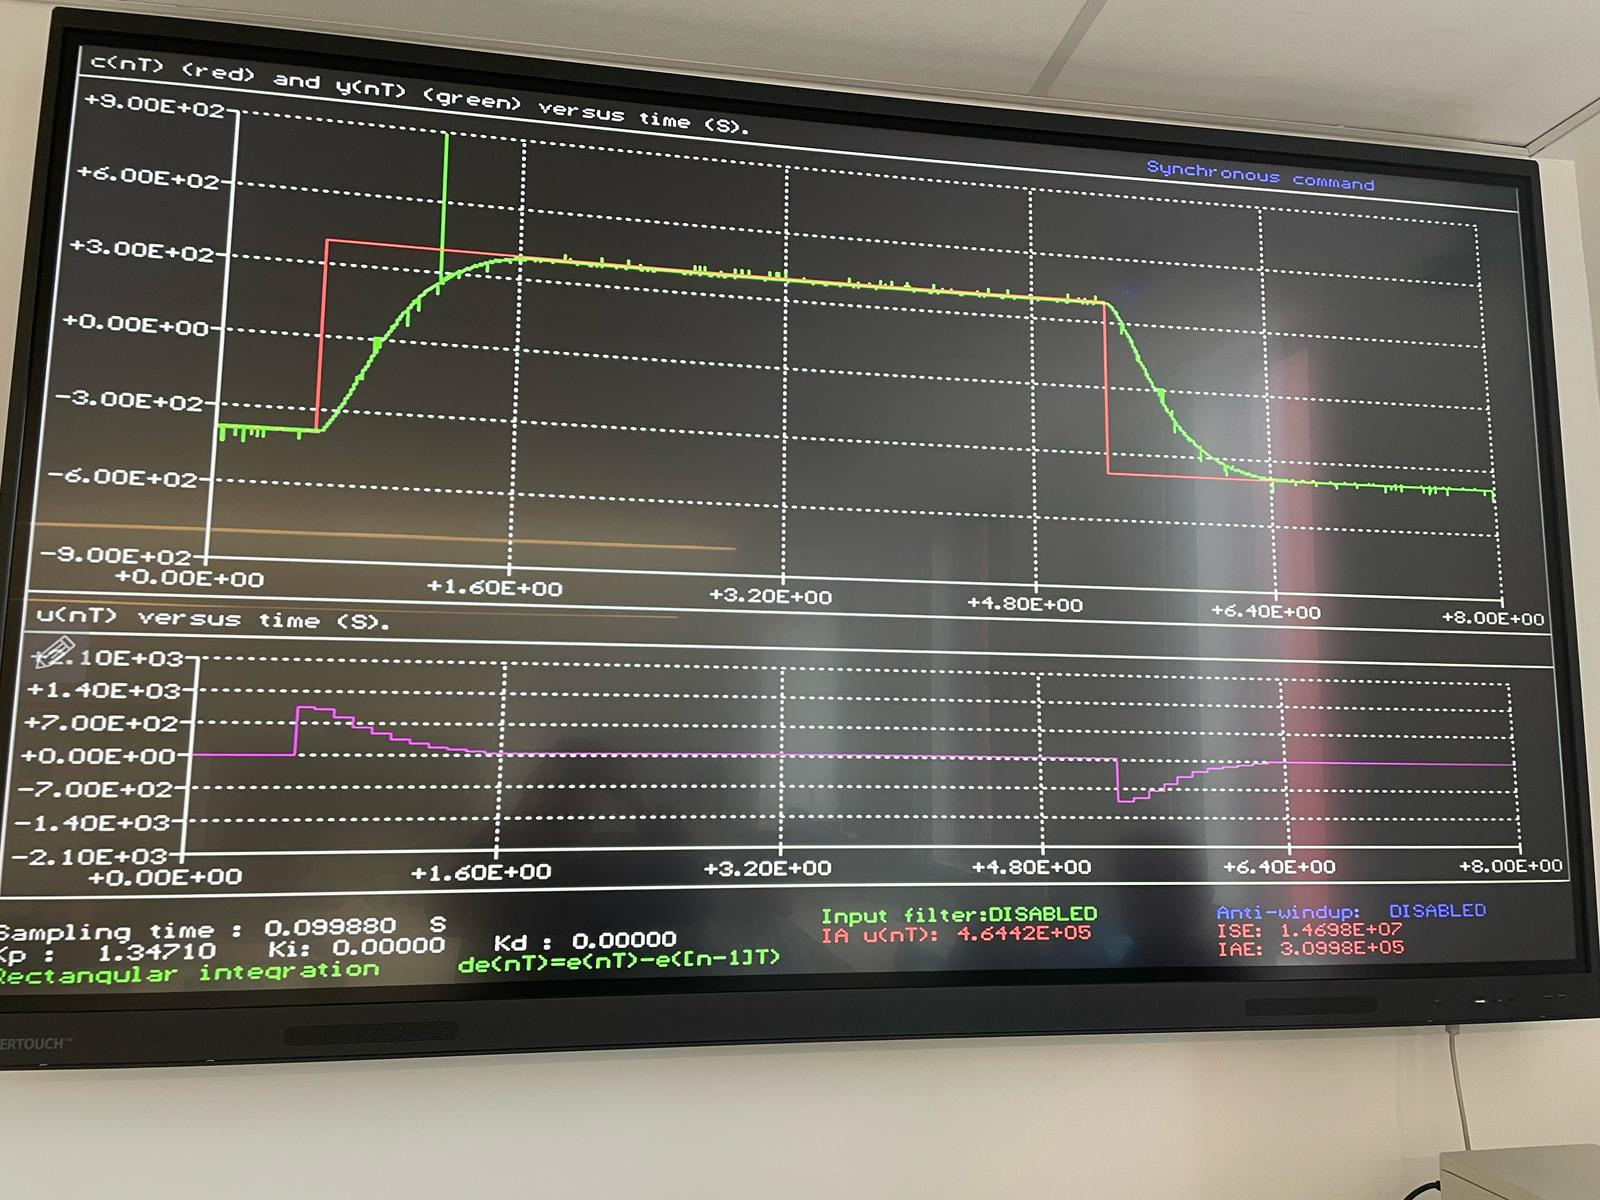
\includegraphics[width=1.1\textwidth]{pictures/task4_kp_0.1_2}
\end{figure}
Figure 1.25 shows a response that is critically damped, but is slightly more damped compared to the response seen in Figure 1.23.
\begin{figure}[H]
    \caption{$T_s = 0.5$, $K_p = 1.3548$: Step Response of Proportional Control - Real DC Servo Rig}
    \label{fig:0.5_Ts_step4_step_response_1}
    \centering
    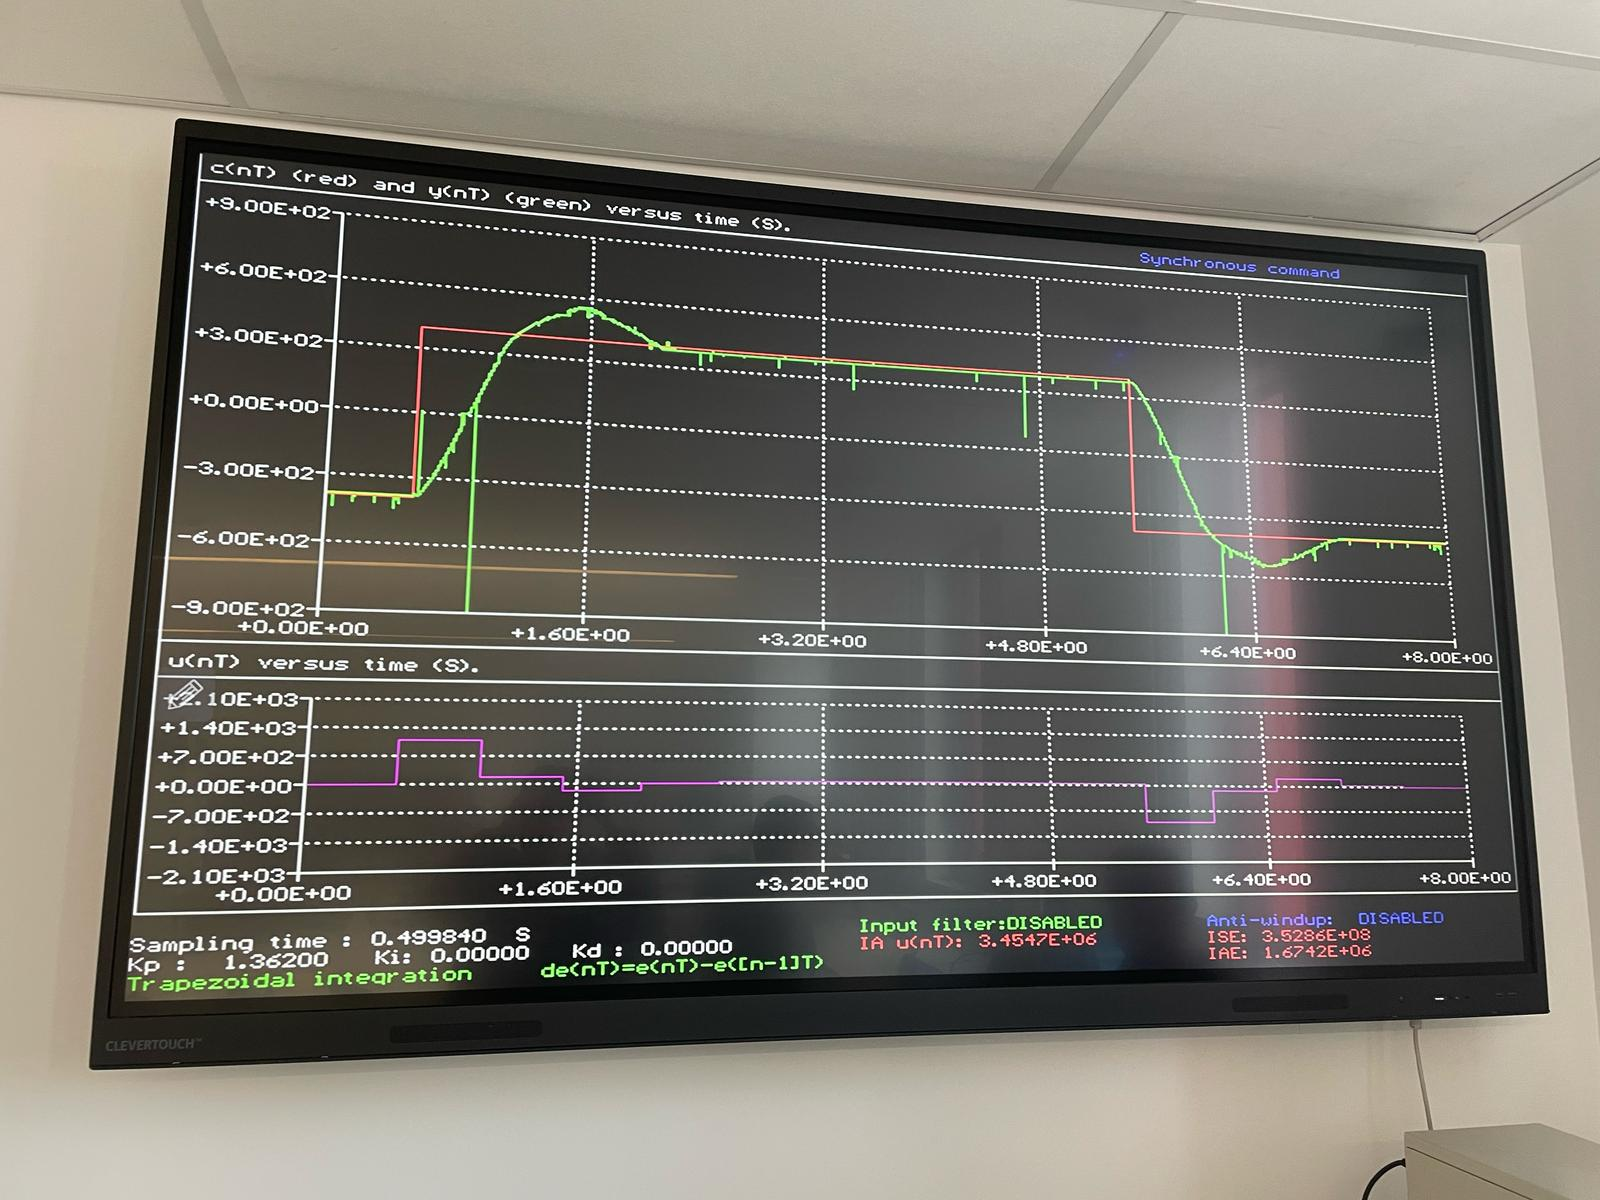
\includegraphics[width=1.1\textwidth]{pictures/task4_kp_0.5_1}
\end{figure}
Figure 1.26 shows a response that is underdamped, the response is far more underdamped comapred with Figure 1.24.
\begin{figure}[H]
    \caption{$T_s = 0.5$, $K_p = 0.7494$: Step Response of Proportional Control - Real DC Servo Rig}
    \label{fig:0.5_Ts_step4_step_response_2}
    \centering
    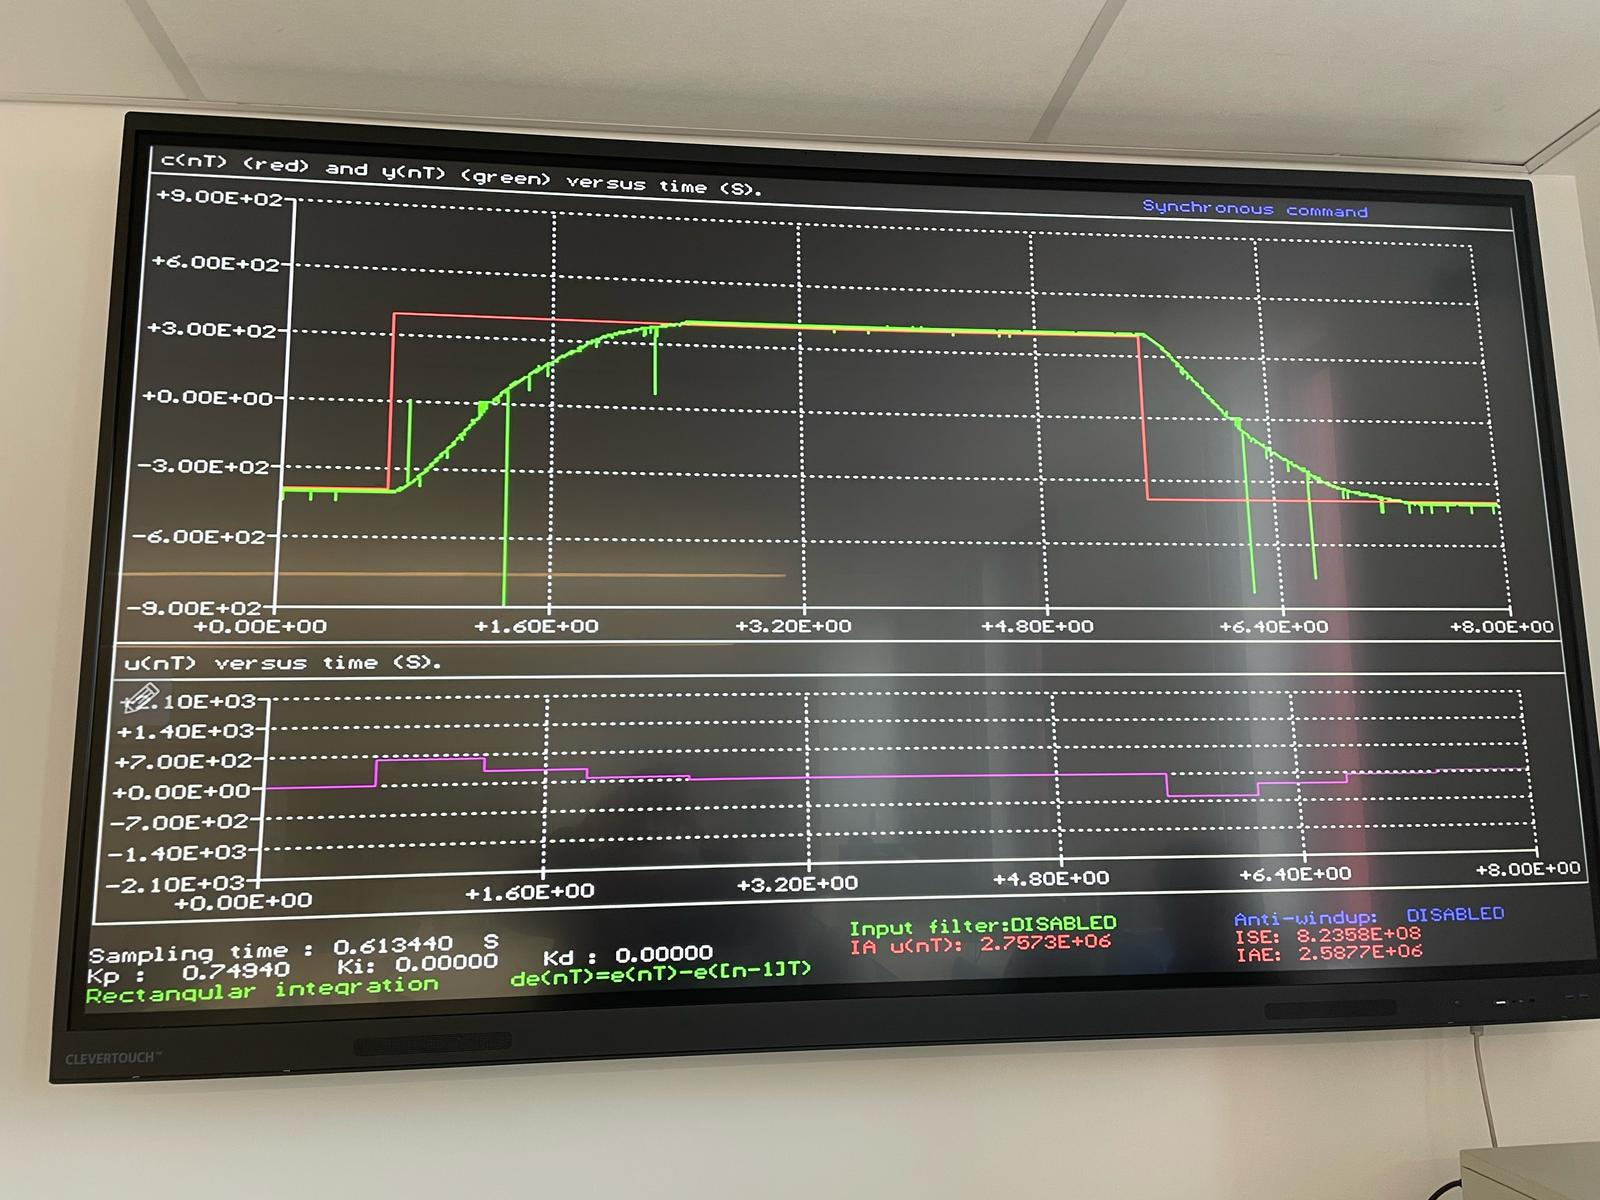
\includegraphics[width=1.1\textwidth]{pictures/task4_kp_0.5_2}
\end{figure}
Figure 1.27 shows a response that is overdamped.
\begin{figure}[H]
    \caption{$T_s = 1.0$, $K_p = 0.8609$: Step Response of Proportional Control - Real DC Servo Rig}
    \label{fig:1.0_Ts_step4_step_response_1}
    \centering
    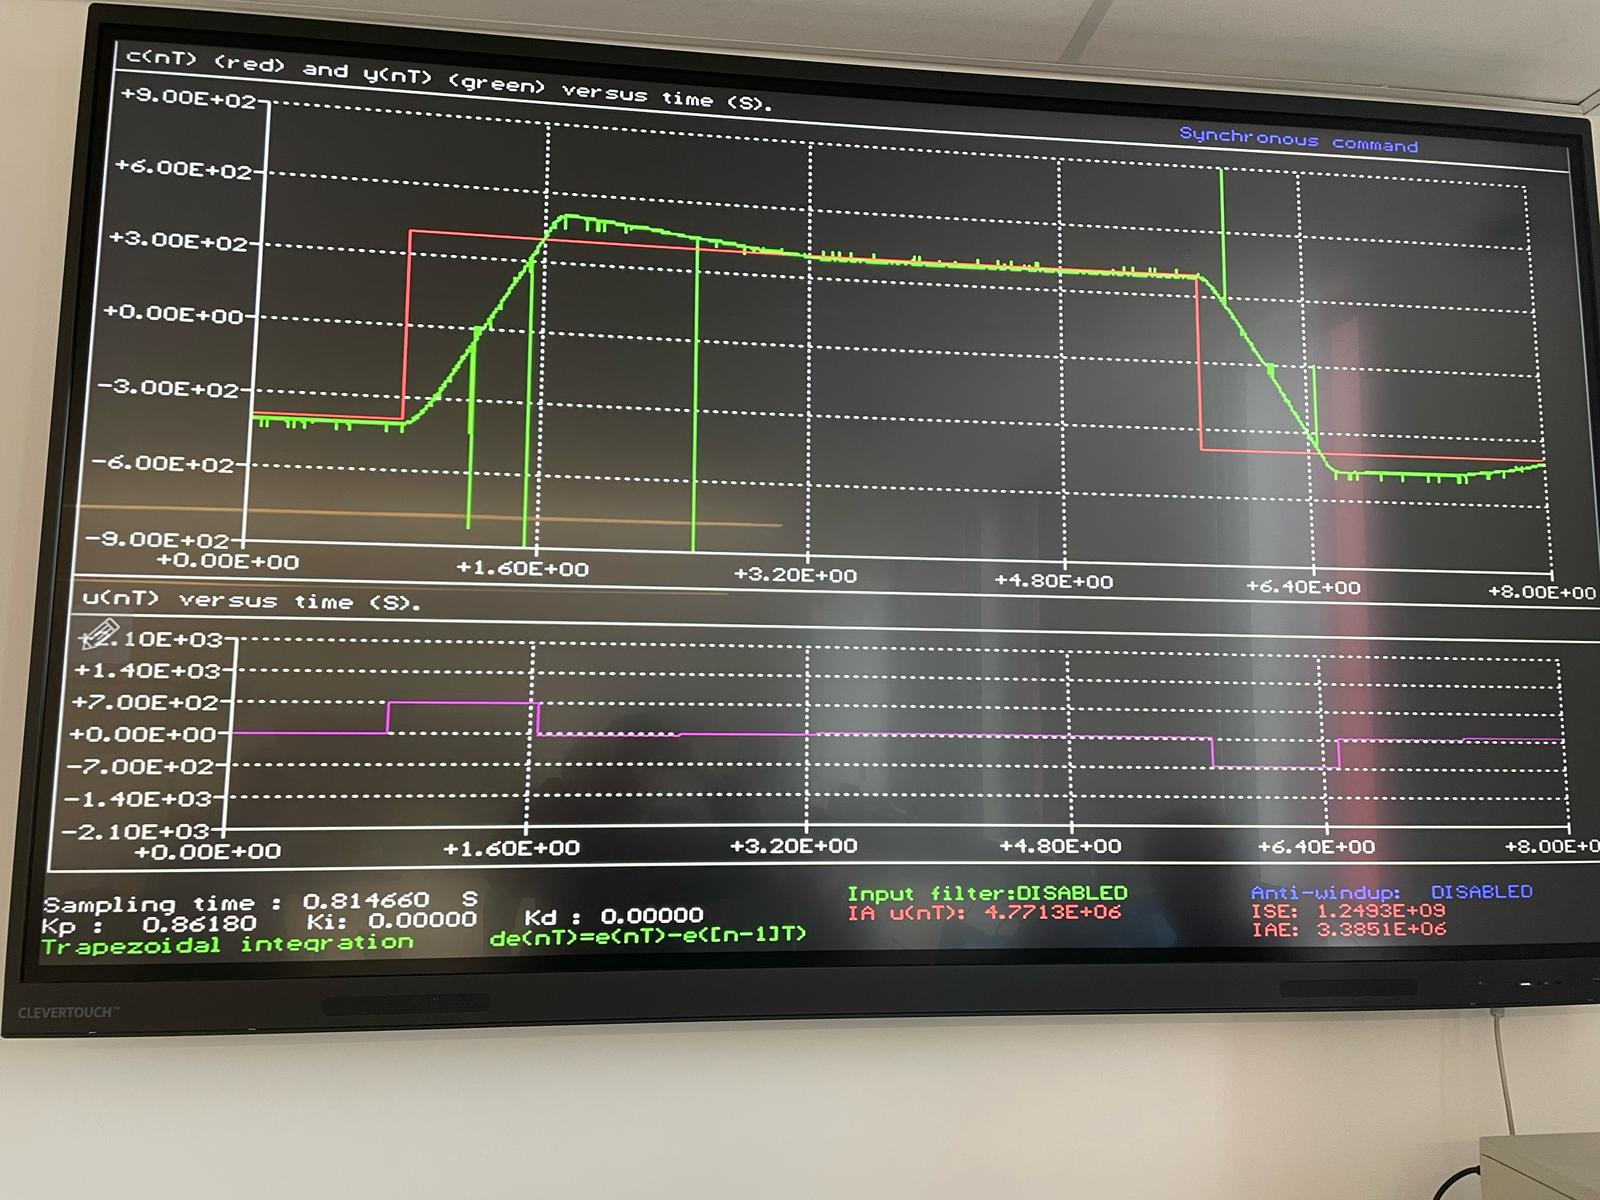
\includegraphics[width=1.1\textwidth]{pictures/task4_kp_1.0_1}
\end{figure}
Figure 1.28 shows a response that is very underdamped and has a very large oscillation before returning to the original value. 
\begin{figure}[H]
    \caption{$T_s = 1.0$, $K_p = 0.4715$: Step Response of Proportional Control - Real DC Servo Rig}
    \label{fig:1.0_Ts_step4_step_response_2}
    \centering
    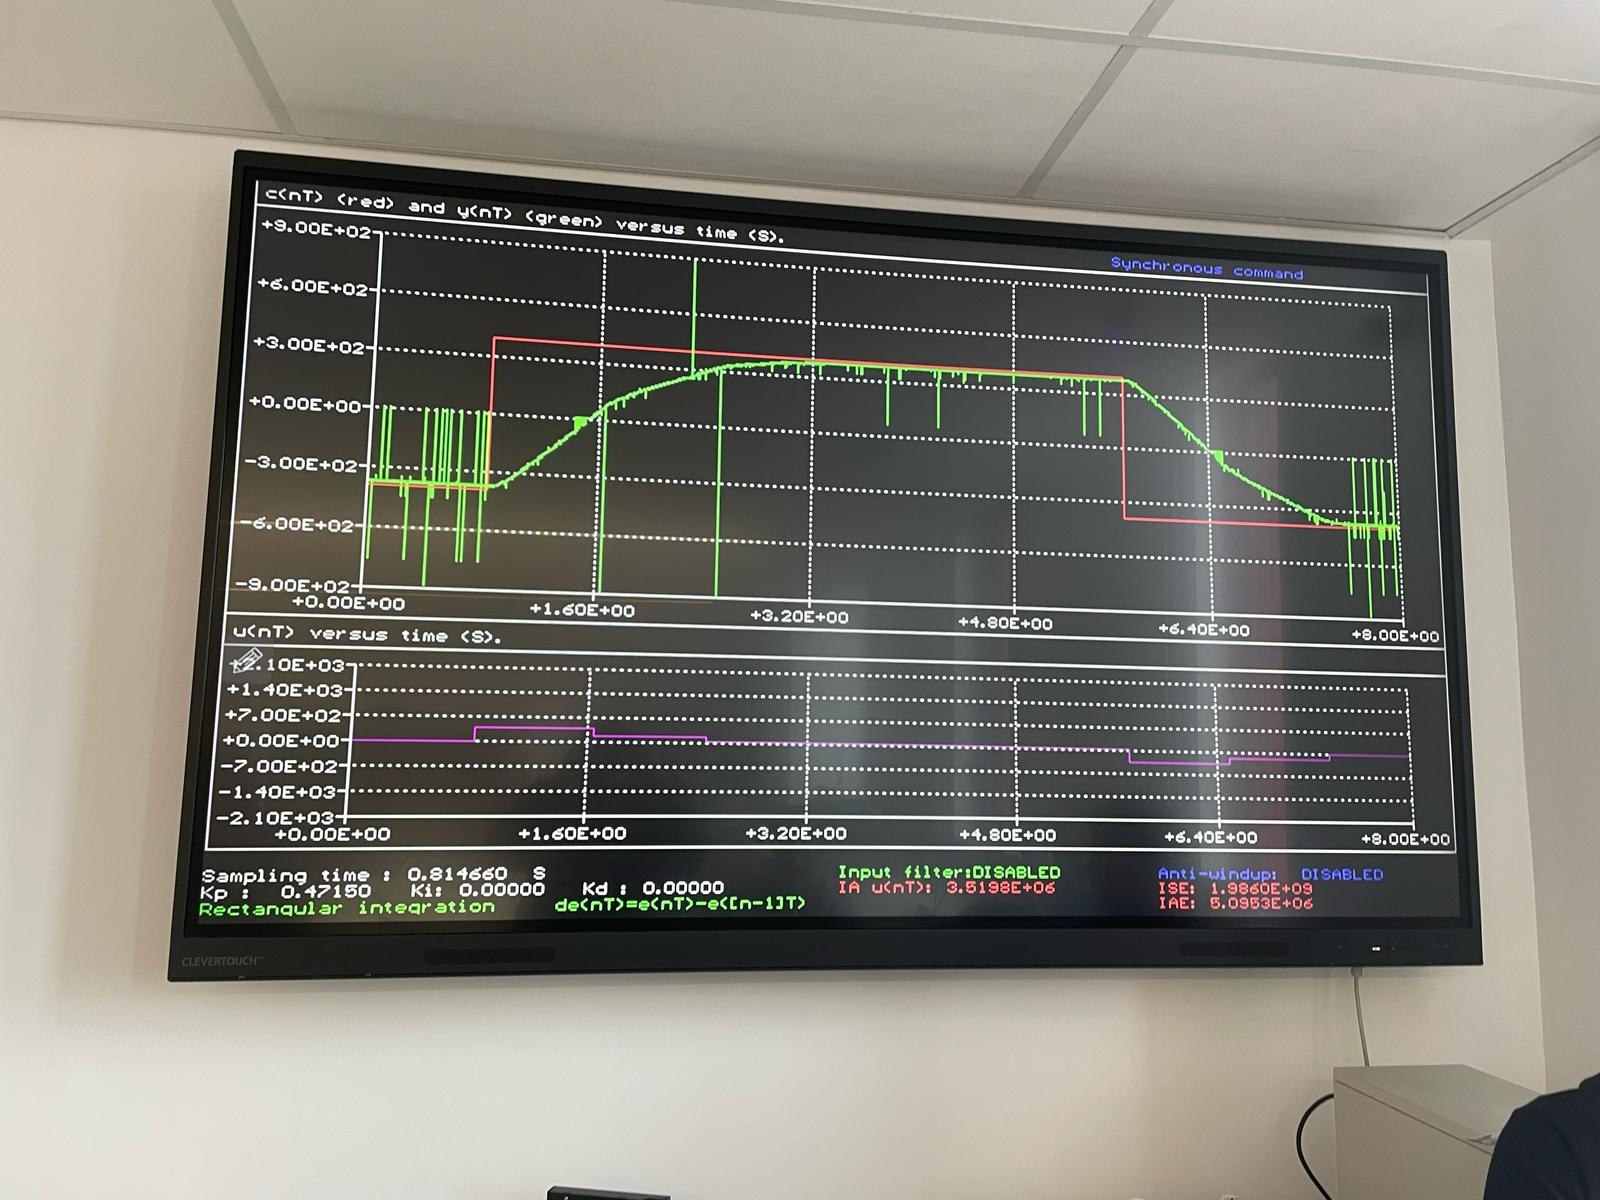
\includegraphics[width=1.1\textwidth]{pictures/task4_kp_1.0_2}
\end{figure}
Figure 1.29 shows a overdamped response, which has been damped more than the response in Figure 1.27.
The following figures, Figures 1.30 (0.01 sample time) and 1.31 (0.1 sample time) will show the responses of the DC Servo rig when being controlled by Digital-Proportional-Derivative control. 
\begin{figure}[H]
    \caption{$T_s = 0.01$, $K_p = 5.7654$, $K_d = 0.1441$: Step Response of Derivative and Proportional Control - Real DC Servo Rig}
    \label{fig:0.01_Ts_step4_step_response_1_PD}
    \centering
    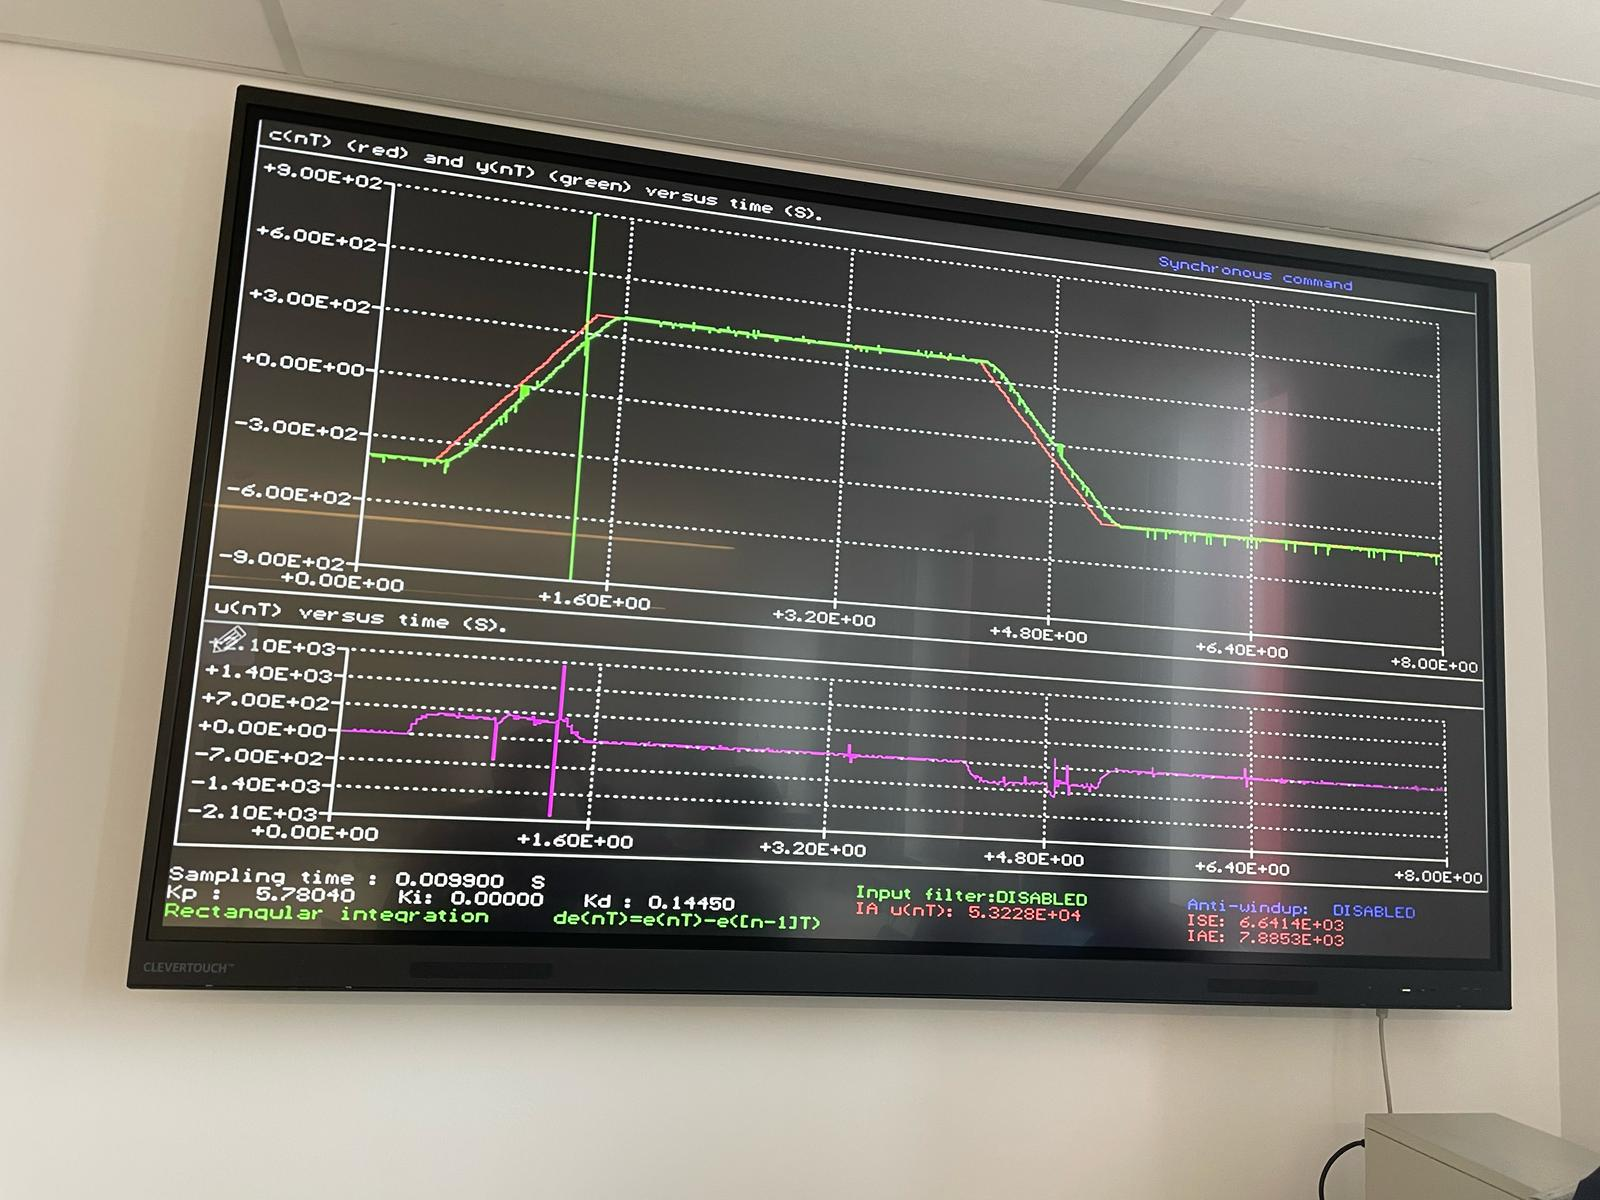
\includegraphics[width=1.1\textwidth]{pictures/task4_kp_kd_1.jpg}
\end{figure}
Figure 1.30 shows a critically damped response.
\begin{figure}[H]
    \caption{$T_s = 0.1$, $K_p = 3.6316$, $K_d = 0.0908$: Step Response of Derivative and Proportional Control - Real DC Servo Rig}
    \label{fig:0.01_Ts_step4_step_response_2_PD}
    \centering
    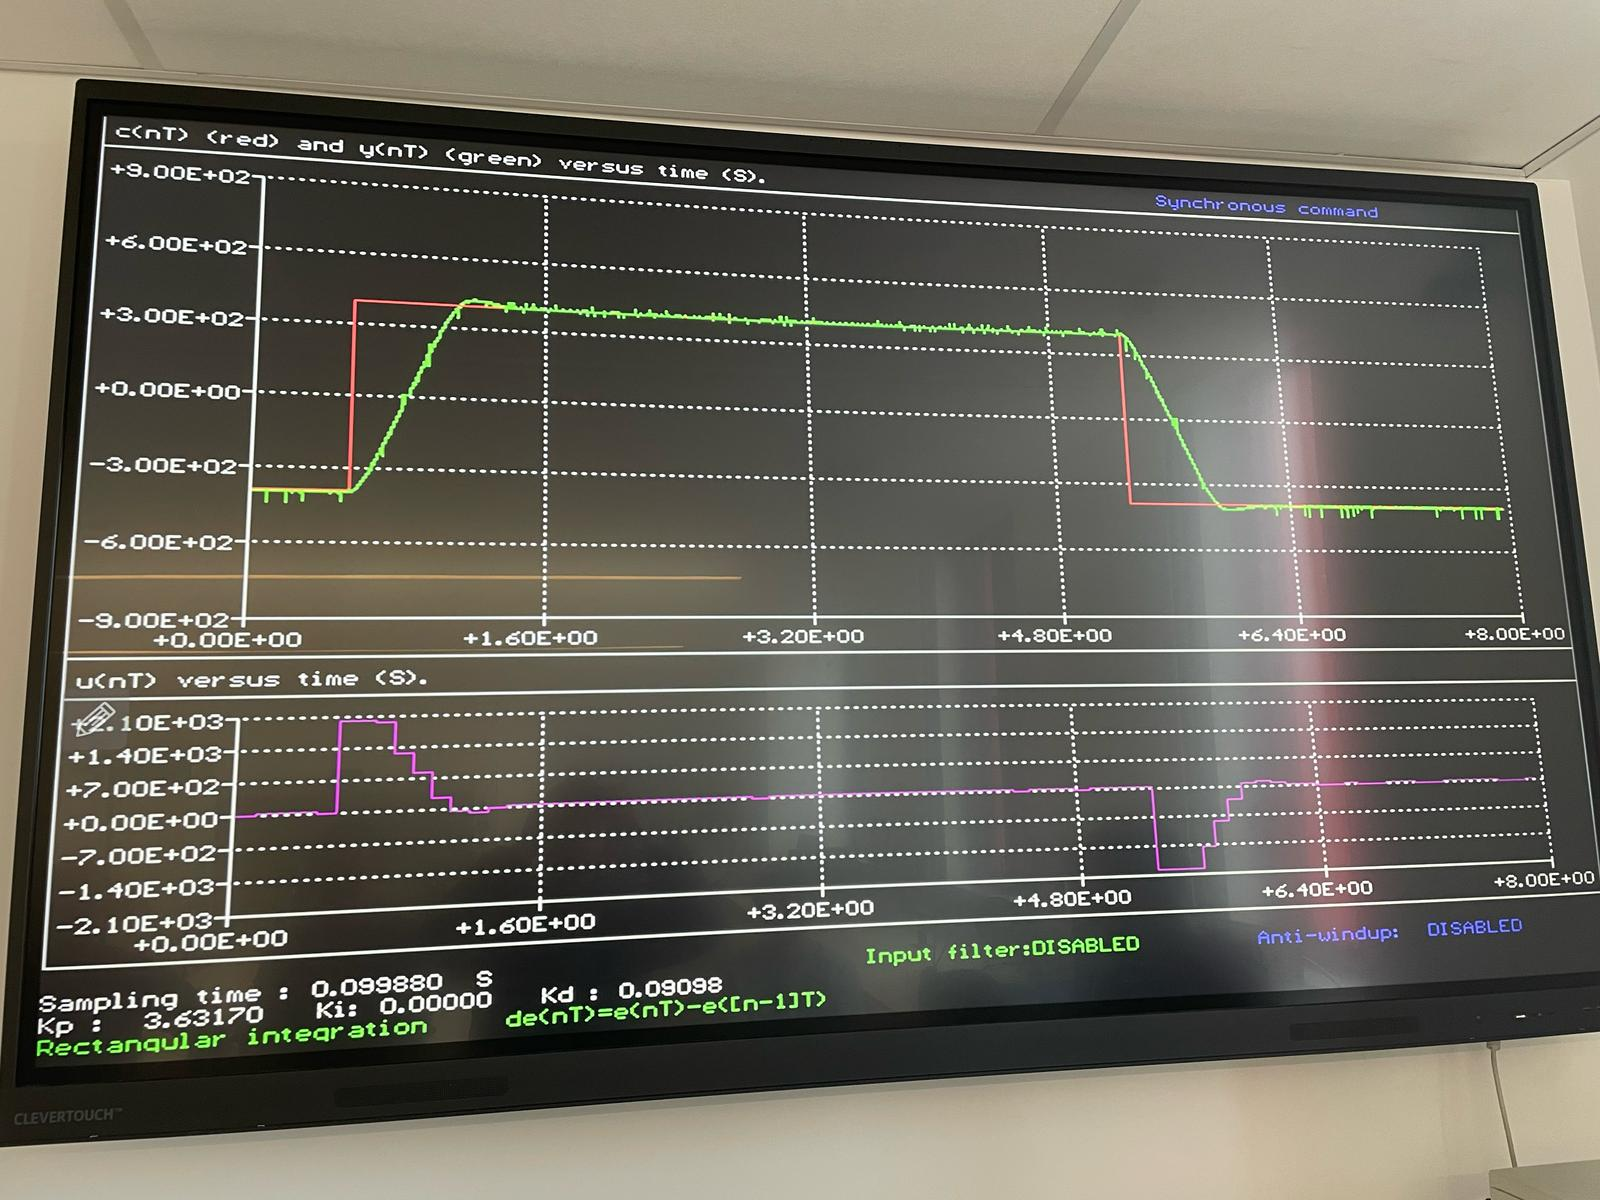
\includegraphics[width=1.1\textwidth]{pictures/task4_kp_kd_2.jpg}
\end{figure}
Figure 1.31 shows a slightly underdamped response.
\subsection{Discussion}
In order for the 4 steps which produced results to be accurate, step 1 has to be completed to a high degree of accuracy. The values for $a$, $b$, $c$ and $h$ were all measured with a cm ruler, with lines drawn on in sharp pencil. Since the measurements are all in mm, each measurement has an accuracy of $\pm 0.05$mm. Any error in this stage could prove to be catastrophic for the accuracy of the whole laboratory. Therefore, the average value was taken of multiple investigators who conducted this same procedure. This makes the values of $k$ and $T$ more accurate. 
Most of the values of $K_p$ estimated on root locus plots in step 2 and 3 were similar (to 2 decimal places) to the values produced by the script itself, and can be seen in Table 1.1 and 1.2. Overall, this suggests there is a good deal of accuracy for the mathematical model produced by the script and the Transfer Functions $G_{ol}$ that it calculates.
For small sample times (0.01 seconds), the step responses are incredibly similar for those produced by the MATLAB script and the real DC Servo rig. However, as the sample time increases, the plots become increasingly "blocky" when produced by MATLAB, however they remain smooth for the real DC Servo rig. Yet, on the real DC Servo responses, there is an increasing number of anomalous readings as the sample size increases. There are no such readings on the sample sizes of 0.01 seconds. This suggests that the DC Servo rig smooths out the response to act over the whole sample time, which in turn produces more erroneous readings. However, the MATLAB simulation produces a more "ideal" response, jumping from output to output, without smoothing over the curve. This makes sense as a real DC Servo rig has to move a physical shaft to produce a response, the simulation does not account for this.   
\subsection{Conclusions}
To conclude, the laboratory was completed successfully by simulating the DC Servo rig within MATLAB and then comparing the results produced with a real DC servo rig. The MATLAB model was proven to be internally consistent as gains produced by the graphs and by mathematics matched up. Furthermore, the overall step responses were very similar for small sample times. However, as the sample time increases, there was a clear difference in the performance of the DC Servo rig and the MATLAB script, which can be explained thanks to the knowledge of how a DC Servo operates  and functions. 
\newpage
\section{Altitude Hold Autopilot Design}
Both safety and efficiency have been significantly improved thanks to the introduction of autopilot systems, which have become an essential aspect of modern aviation. Initially, autopilots were introduced to reduce the flight crew’s workload during long-haul flights but over time they have evolved into highly sophisticated systems, which are capable of completing various complex tasks autonomously. One of the different functionalities of autopilots is altitude hold. This feature is of paramount importance for safety and efficiency, as it ensures a steady and controlled flight path is followed, this means that the desired cruising altitude is maintained. Any deviation in the desired cruising altitude could result in serious safety concerns, the aircraft could come into conflict, and cause fuel inefficiencies, thus reducing profit margins for airlines. \newline

The primary function of altitude hold in autopilots is to maintain a specific altitude, autonomously; this allows pilots to focus on other critical aspects of flight, including communicating with air traffic control. This is vitally important for long flights, as small deviations in altitude accumulate over time, resulting in a very significant altitude change (\cite{nasa2017}). This is especially important when flying through turbulence, which can drastically change the aircraft’s altitude in a very short period of time, this turbulence is also very frequently encountered between 30kft and 40kft (the altitude range of most modern airliners) (\cite{nasa2017}). Altitude hold systems will automatically account for these altitude changes, returning the aircraft to equilibrium; the best autopilot systems do this quickly and efficiently (with as few oscillations as possible).

\newpage

\subsection{Objectives and Theory}

\subsubsection{Objectives}
The key objectives of any altitude hold system are: 
\begin{enumerate}
    \item To maintain a fixed altitude, which ensures compliance with Air Traffic Control regulations.
    \item Minimise pilot workload, by providing automatic altitude maintenance during cruise flight.
    \item Enhance flight stability, by reducing oscillations due to atmospheric disturbances and therefore, improving passenger comfort.
    \item Creating smooth transitions when changing altitude, which improves fuel efficiency. 
\end{enumerate}

\subsubsection{Theory}

The altitude hold system is modelled using the two degrees of freedom linear equations of motion, which describe aircraft longitudinal dynamics. They are given by

\begin{equation}
    {\dot w} = \overline Z_{w} w+ V_{R}q+\overline  Z_{\eta } \eta \, , 
\end{equation}
\label{eq:2.1}
\myequations{Two DOF Linear Equation of Motion 1}

\begin{equation}
    {\dot q}- \overline M_{ {\dot w} }{\dot w}=\overline  M_{w}w+ \overline M_{q}q+ \overline  M_{\eta } \eta \, ,
\end{equation}
\label{eq:2.2}
\myequations{Two DOF Linear Equation of Motion 2}

\begin{equation}
    q={\dot \theta} \, ,
\end{equation}
\label{eq:2.3}
\myequations{Two DOF Linear Equation of Motion 3}

\begin{equation}
    {\dot h}=  V_{R} \theta -w \, ,
\end{equation}
\label{eq:2.4}
\myequations{Two DOF Linear Equation of Motion 4}

These equations describe how the aircraft’s vertical velocity (w), pitch rate (q) and altitude (h) change due to control surface deflections ($\eta$). From these equations, transfer functions in the laplace domain can be derived

\begin{equation}
    G^{q}_{\eta}(s)=  {{(\overline M_{\eta}+\overline M_{\dot w}\overline Z_{\eta})s+(\overline M_{w}\overline Z_{\eta}-\overline M_{\eta}\overline Z_{w})}\over{s^2-(V_{R}\overline M_{\dot w}+\overline Z_{w}+\overline M_{q})s+(\overline M_{q}\overline Z_{w}-V_{R}\overline M_{w})}} \, , 
\end{equation}
\label{eq:2.5}
\myequations{Transfer Function: How Elevator Deflection Impacts Pitch Rate}

Equation 2.5 describes how elevator deflection affections pitch rate.

\begin{equation}
    G^{\theta}_{\eta}(s)=  {{1}\over{s}}  \cdot G^{q}_{\eta} \, ,
\end{equation}
\label{eq:2.6}
\myequations{Transfer Function: How Elevator Deflection Impacts Pitch Angle}

Equation 2.6 describes how elevator deflection affects pitch angle.

\begin{equation}
    G^{h}_{\theta}(s)=  {{1}\over{s}}  \cdot  {{-\overline Z_{\eta}s^2+(\overline M_{q}+V_{R}\overline M_{\dot w})\overline Z_{\eta}s+V_{R}(\overline M_{w}\overline Z_{\eta}-\overline M_{\eta}\overline Z_{w})}\over{(\overline M_{\eta}+\overline M_{\dot w}\overline Z_{\eta})s+(\overline M_{w}\overline Z_{\eta}-\overline M_{\eta}\overline Z_{w})}} \, , 
\end{equation}
\label{eq:2.7}
\myequations{Transfer Function: How Pitch Angle Impacts Altitude}

Equation 2.7 describes how pitch angle affects altitude. \newline

The autopilot system has been designed using a sequential loop closure approach, with two distinct stages. The first is the design of a pitch attitude hold system, which is made up of the two inner loops seen in Figure 2.1. The second is the closure of the feedback loop around the pitch attitude hold system; again as seen in Figure 2.1.

\begin{figure}[H]
    \caption{Block diagram of an Altitude Hold System.}
    \label{fig:block_diagram_altitude_hold}
    \centering
    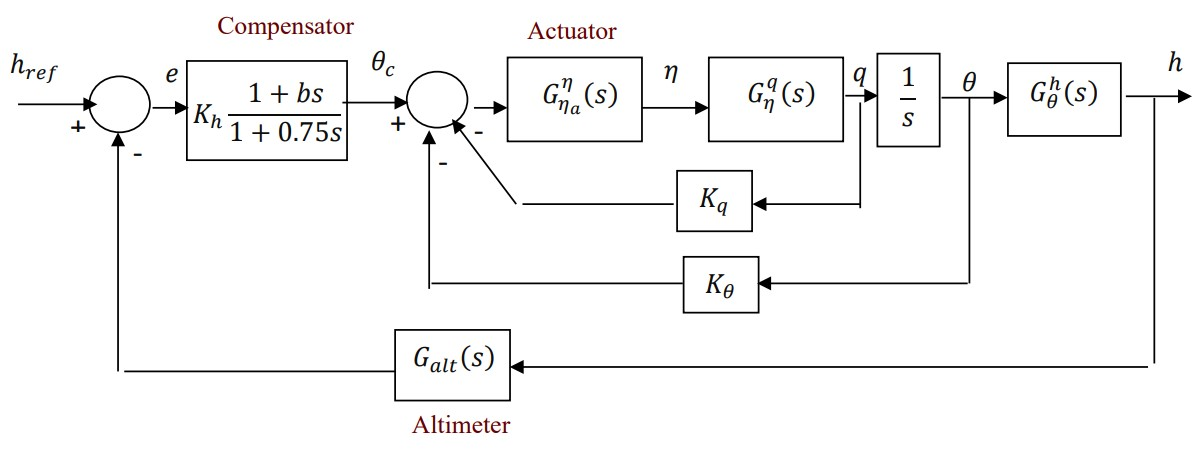
\includegraphics[width=1.1\textwidth]{pictures/figure 2.1.jpg}
\end{figure}

The first stage (inner loops) is responsible for regulating pitch attitude. It consists of both a pitch rate feedback loop, which damps excessive pitch rate variations, and a pitch angle feedback loop, which ensures the aircraft maintains required altitude by adjusting the elevator control. The closed loop transfer function for the pitch attitude design is derived by root locus design, to achieve a damping ratio of 0.5 and natural frequency of 3 rad/s. This is achieved as follows:

\begin{equation}
    s_{1} = -\sigma + j\omega_{d} \, ,
\end{equation}
\label{eq:2.8}
\myequations{Complex Number $s_1$}
\begin{equation}
    \sigma = \zeta\omega_{n} \, ,
\end{equation}
\label{eq:2.9}
\myequations{$\sigma$ In Terms of $\zeta$ and $\omega_n$}
\begin{equation}
    \omega_{d} = \omega_{n}\sqrt{1-\zeta^2} \, ,
\end{equation}
\label{eq:2.10}
\myequations{$\omega_d$ In Terms of $\zeta$ and $\omega_n$}

When $\zeta$ takes the value of 0.5 and $\omega_{n}$ takes the value of 3, $s_{1}=-1.5+2.5981j$.\newline

Then, a compensator zero is placed at $s=-a$ so that the desired pole lies on the root locus. This is achieved by first reducing the block diagram shown in Figure 2, by replacing $G^\eta_{\eta_{a}}$ and $G^q_{\eta}$ with transfer function $G_{p}$. Finally transfer function $G_{1}$ can be found by dividing by $s$:

\begin{equation}
    G_{1} (s)={{G_{p}}\over{s_1}} \, ,
\end{equation}
\label{eq:2.11}
\myequations{Transfer Function $G_1$ - used to find compensator zero.}

Finally, the value of $a$ can be determined by ensuring that the sum of $a$ and the angle of $s_1$ multipled by the angle of $G_1$ is equal to $\pi$. This can be expressed mathematically as:

\begin{equation}
    \angle{((s_1+a)G_1 (s))}=\pi \, ,
\end{equation}
\label{eq:2.12}
\myequations{Expression for finding $a$}

With the compensator pole in place, values of the gains $K_q$ and $K_{\theta}$ can be obtained, so that the closed-loop transfer function of the pitch attitude control system can be found.

\begin{equation}
    K_q={{1}\over{|G_1(s_1)|}} \, ,
\end{equation}
\label{eq:2.13}
\myequations{Equation for gain $K_q$}
\begin{equation}
    K_{\theta}=aK_q \, ,
\end{equation}
\label{eq:2.14}
\myequations{Equation for gain $K_{\theta}$}

So the closed-loop transfer function of the pitch attitude system is:

\begin{equation}
    G^{\theta}_{\theta_{c}}={{G_1 (s)}\over{1+K_q(s+a)G_1 (s)}} \, ,
\end{equation}
\label{eq:2.15}
\myequations{Transfer Function $G^{\theta}_{\theta_{ref}}$ - CLTF of pitch attitude system.}

The denominator of the transfer function in Equation 2.15 is the characteristic equation of the pitch attitude system. This means that the zero of the system is located at  $s=-a$, with point $s_1$ lying on the root locus branch for the open loop transfer function: 

\begin{equation}
    G_2(s_1) = (s+a)G_1 (s) \, ,
    \label{eq:2.16}
\end{equation}
\myequations{Transfer Function $G_2$ - OLTF of pitch attitude system.}

This transfer function should also satisfy the root locus criterion, as the angular value should be exactly equal to $\pi$.

The second stage (outer loop) regulates the aircraft’s altitude by adjusting the pitch attitude. The altimeter provides altitude feedback, and a compensator adjusts the pitch command to correct altitude deviations. The altitude loop is only closed after designing the pitch control loop, so that appropriate pitch commands are generated, and then executed by the inner loop. Therefore, since the transfer function for the inner loop has been set (Equation 2.15) the design for the outer loop can be determined by block diagram reduction, as seen in Figure 2.2.

\begin{figure}[H]
    \caption{Simplified block diagram for the altitude hold loop (outer loop).}
    \label{fig:block_diagram_simplified_altitude_hold}
    \centering
    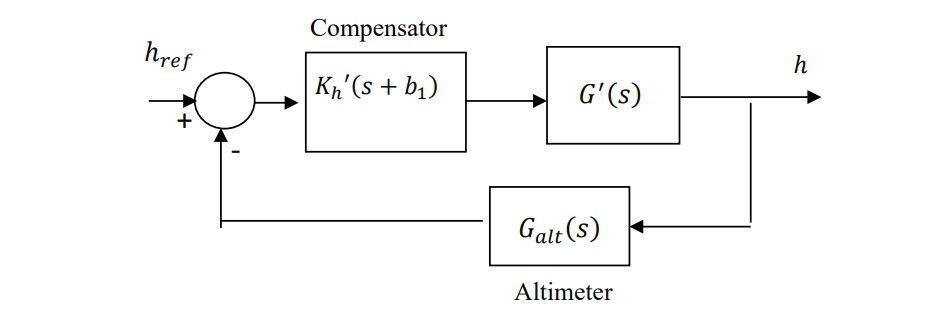
\includegraphics[width=1.1\textwidth]{pictures/figure 2.2.jpg}
\end{figure}

Where: 

\begin{equation}
    G^{\prime}= ({{1}\over{1+0.75s}})G^{\theta}_{\theta_{c}}(s)G^h_{\theta}(s) \, ,
    \label{eq:2.17}
\end{equation}
\myequations{Transfer Function $G^{\prime}$}

And: 

\begin{equation}
    G^*(s)=G^{\prime}(s)G_{alt}(s) \, ,
    \label{eq:2.18}
\end{equation}
\myequations{Transfer Function $G^{*}$}

Terms $K_h^{\prime}$ and $b_1$ are to be determined, however transfer function $G_{alt}(s)$ has known properties as the performance of the aircraft's elevators have been measured.

\begin{equation}
    G_{alt}(s)={{10}\over{s+10}} \, ,
    \label{eq:2.19}
\end{equation}
\myequations{Transfer Function $G_{alt}$}

For the outer loop, an identical method, to what was used in the inner loop, is used to design a root locus. The only difference is that we solve with complex number $s_2$ by using a $\zeta$ of 0.5 and a $\omega_n$ of 0.5 rad/s. Therefore, by recalling Equations 2.8, 2.9 and 2.10, the complex number $s_2$ is found. Therefore, a compensator zero can be placed when $s=b_1$, which can be found by slightly modifying Equation 2.12:

\begin{equation}
    \angle{((s_2+b_1)G^* (s_2))}=\pi \, ,
\end{equation}
\label{eq:2.20}
\myequations{Expression for finding $b_1$}

Once a suitable $b_1$ has been determined, the transfer function $G_3(s_2)$ can be determined, by taking $G_{alt}$ and multiplying by $(s+b_1)$, which now includes our compensator zero in the transfer function. This means that, the value of the gains $K_h^{\prime}$ and $K_h$ can be found by direct calculation:

\begin{equation}
    K_h^{\prime}={{1}\over{|G_3(s2)}} \, ,
\end{equation}
\label{eq:2.21}
\myequations{Expression for finding $K_h^{\prime}$}
\begin{equation}
    K_h={{K_h^{\prime}}\over{b_1}} \, ,
\end{equation}
\label{eq:2.22}
\myequations{Expression for finding $K_h$}

Additionally, just like for $G_2(s_1)$ the angular value of the transfer function $G_3(s2)$ should be exactly equal to $\pi$. 

Now, all unknown terms have been evaluated, including the gains used in the Compensator block in Figure 2.2. This means that the outer loop can be closed around the inner loop, completing the theoretical altitude hold design. The simplified closed loop transfer function is:

\begin{equation}
    G_{h_c}^h(s)={{K_h^{\prime}(s+b_1)G^{\prime}}\over{1+G_3(s_2)K_h^{\prime}}} \, ,
\end{equation}
\label{eq:2.23}
\myequations{Closed loop transfer function of the altitude hold system.}

It's important to note the key relationship between the two loops: the inner loop must be fast and stable to respond effectively to pitch commands from the outer loop, whereas, the outer loop uses the inner loop to influence the altitude, but operates slower to avoid excessive oscillations. 

\subsection{Modelling and Results}
\subsubsection{Modelling}
The mathematical modelling of the altitude hold system was completed inside of a MATLAB environment, with two distinct scripts (.m files). One of these files is responsible for handling all variables that will be used throughout the course of the design process. The second file contains the mathematical model of the altitude hold system as outlined previously. 

Storing the variables in a different script provides a great deal of flexibility, as changing one line of code will enable the user to simulate the autopilot hold system in different conditions, without having to manually change each aerodynamic and control derivative. Variable files are stored in the following format:

\begin{lstlisting}[language=MATLAB]
    %%% Workspace Cleanup %%%
    clc;
    clear;
    close all;
    
    s = tf('s');
    %%% Stability and Control Derivatives and Flight Condition %%%
    [Xu, Zu, Mu, Xw, Zw, Mw, Xw_dot, Zw_dot, Mw_dot, Xq, Zq, Mq, Xeta, Zeta, Meta, VR, g] = final_assignment_variables(); % Change the name of this function to to run this system with different variable values.
    
    %%% Actuator and Altimeter Dynamics %%%
    G_etaA_eta = -4/(s+4);
    G_etaA_eta_Numerator = cell2mat(G_etaA_eta.Numerator); % Gets numerator in appropriate form for Simulink
    G_etaA_eta_Denominator = cell2mat(G_etaA_eta.Denominator); % Gets denominator in appropriate form for Simulink
    G_alt = 10/(s+10);
    G_alt_Numerator = cell2mat(G_alt.Numerator); % Code relevant to SIMULINK
    G_alt_Denominator = cell2mat(G_alt.Denominator); % Code relevant to SIMULINK
    
    %%% Transfer Functions - TASK 1 %%% 
    G_eta_q = ((Meta + (Mw_dot*Zeta))*s + ((Mw*Zeta) - (Meta*Zw)) )/((s^2) - ((VR*Mw_dot) + Zw + Mq)*s +((Mq*Zw) - (VR*Mw)));
    G_eta_q_Numerator = cell2mat(G_eta_q.Numerator); % Gets numerator in appropriate form for Simulink
    G_eta_q_Denominator = cell2mat(G_eta_q.Denominator); % Gets denominator in appropriate form for Simulink
    G_eta_theta = 1/s * G_eta_q;
    G_theta_h = 1/s * ((-Zeta*(s^2))+ Zeta*s*(Mq+VR*Mw_dot) + VR*(Mw*Zeta-Meta*Zw))/(s*(Meta+Mw_dot*Zeta) + (Mw*Zeta-Meta*Zw));
    Gp = G_etaA_eta*G_eta_q;
    G1 = Gp/s;
    
    %%% Root Locus Design for Pitch Control - TASK 2 %%%
    Wn = 3; % Specified in brief
    zeta = 0.5; % Specified in brief
    sigma = zeta*Wn;
    Wd = Wn*sqrt(1-zeta^2);
    s1 = -sigma + 1i * Wd; % Complex number s1 is designed based on parameters decided in the brief. This complex is used as a design goal for G2
    
    %%% Plot The Root Locus for Pitch Control - TASK 3 %%%
    figure;
    rlocus(G1)
    hold on;
    plot(real(s1), imag(s1), 'rx', 'MarkerSize', 10, 'LineWidth', 2);
    title('Root Locus of G1(s) - Pitch Control');
    grid off;
    
    %%% Evaluating the Complex Number of G1 - TASK 4 %%%
    G1_s1 = evalfr(G1, s1);
    mag_G1_s1 = abs(G1_s1);
    angle_G1_s1 = angle(G1_s1);
    
    %%% Find the location of the compensating Zero - TASK 5 %%%
    alpha_c = pi - angle_G1_s1;
    a = sigma + Wd / tan(alpha_c); % Finds the zero location, a, by accounting for the phase shortfall at point s1. 
    % The goal of this step is to move the root locus branch to co-inside with
    % the complex number s1. "a" is a constant determined which wil be
    % multiplied by G1 to achieve this.
    
    %%% Define G2 and show the point s1 on it's Root Locus Plot - TASK 6 %%%
    G2 = (s+a)*G1;
    G2_s1 = evalfr(G2, s1);
    angle_G2_s1 = angle(G2_s1); % May output a value close to, but not exactly pi - the criterion should still be met.
    fprintf('The phase of G2 at s1 is: %.4f radians\n', abs(angle_G2_s1));
    figure;
    rlocus(G2);
    hold on;
    plot(real(s1), imag(s1), 'rx', 'MarkerSize', 10, 'LineWidth', 2);
    title('Root Locus of G2(s) - Pitch Control');
    grid off;
    
    %%% Check to see if the angle criterion is satisfied %%%
    if abs(abs(angle_G2_s1) - pi) < 1e-3
        disp('The angle criterion has been satisfied for G2 at s1 - the phase is approximately pi.');
    else
        disp('The angle criterion has not been satisfied.');
    end
    
    %%% Calculating the Gains - TASK 7 %%%
    Kq = 1/(abs(G2_s1)); % Kq*mag_G1_s1 = 1. This satisfies the magnitude condition at s1. This means the CL pole will be at s1. 
    Ktheta = a*Kq; % Therefore, Krg = Kq.
    
    %%% Determine the CLTF and find the Zeros and Poles - TASK 8 %%%
    G_theta_c = feedback(G1,Kq*(s+a));
    
    info = stepinfo(G_theta_c*5); % Gets the properties from the CLTF with a step change of 5 degrees.
    overshoot = info.Overshoot;       % Percentage overshoot of CLTF
    settlingTime = info.SettlingTime;   % Settling time in seconds of CLTF
    finalValue = dcgain(G_theta_c*5);      % Final value of CLTF
    
    figure;
    [response, time] = step(G_theta_c*5);
    plot(time, response, 'LineWidth',2);
    
    [maxVal, maxIdx] = max(response); 
    maxTime = time(maxIdx); % Find the maximum response value and its time
    
    grid on;
    title('Step Response of Pitch Attitude Control - Pitch Control');
    
    annotationStr = sprintf('Maximum Overshoot: %.2f%%\nSettling Time: %.2f s\nFinal Value: %.2f', overshoot, settlingTime, finalValue); % Creates the annotation text with variable placeholders.
    
    annotation('textbox', [0.3, 0.3, 0.3, 0.2], 'String', annotationStr, 'FitBoxToText', 'on', 'BackgroundColor', '#ADD8E6', 'EdgeColor', 'black', 'FontSize', 50); % Creates the annotation with a text box.
    
    pole_G_altitude = pole(G_theta_c);
    zero_G_altitude = zero(G_theta_c);
    disp('The poles of G_theta_c are:');
    disp(pole_G_altitude);
    disp('The zeros of G_theta_c are:');
    disp(zero_G_altitude);
    
    %%% Define Altitude Loop Transfer Functions - TASK 9 %%%
    a_c = 0.75;
    G_prime = (1 / (1 + a_c*s)) * G_theta_c * G_theta_h; 
    G_star = G_prime * G_alt;
    
    %%% Root Locus Design for Altitude Control - TASK 10 %%%
    Wn_2 = 0.5;
    zeta_2 = 0.5;
    sigma_2 = zeta_2*Wn_2;
    Wd_2 = Wn_2*sqrt(1-zeta_2^2);
    s2 = -sigma_2 + 1i * Wd_2;
    
    %%% Plot the Root Locus for Altitude Control - TASK 11 %%%
    figure;
    rlocus(G_star);
    hold on;
    plot(real(s2), imag(s2), 'rx', 'MarkerSize', 10, 'LineWidth', 2);
    title('Root Locus of G*(s) - Altitude Control');
    grid off;
    
    %%% Evaluating the Complex Number of G_star - TASK 12 %%%
    G_star_s2 = evalfr(G_star, s2);
    mag_G_star_s2 = abs(G_star_s2);
    angle_G_star_s2 = angle(G_star_s2);
    
    %%% Compute Zero Location for Altitude Control - TASK 13 %%%
    alpha_c_prime = pi - angle_G_star_s2;
    b1 = sigma_2 + Wd_2 / tan(alpha_c_prime);
    
    %%% Define G3(s) and Root Locus Plot for Altitude Control - TASK 14 %%%
    G3 = (s + b1) * G_star;
    G3_s2 = evalfr(G3, s2);
    angle_G3_s2 = angle(G3_s2);
    fprintf('The phase of G3 at s2 is: %.4f radians\n', abs(angle_G3_s2));
    figure;
    rlocus(G3);
    hold on;
    plot(real(s2), imag(s2), 'rx', 'MarkerSize', 10, 'LineWidth', 2);
    title('Root Locus of G3(s) - Altitude Control');
    grid off;
    
    %%% Check to see if the angle criterion is satisfied %%%
    if abs(abs(angle_G3_s2) - pi) < 1e-3
        disp('The angle criterion has been satisfied for G3 at s2 - the phase is approximately pi.');
    else
        disp('The angle criterion has not been satisfied.');
    end
    
    %%% Calculate the gain Kh_prime - TASK 15 %%%
    kh_prime = 1/abs(G3_s2);
    
    %%% Calculate the gain Kh - TASK 16 %%%
    kh = kh_prime * b1;
    
    %%% Compute Closed Loop Transfer Function - TASK 17 %%%
    G_altitude = feedback(kh*(s+b1)*G_prime, G_alt);
    
    info_2 = stepinfo(50 * G_altitude); % Gets the properties from the CLTF with a step change of 5 degrees.
    overshoot_2 = info_2.Overshoot;       % Percentage overshoot of CLTF
    settlingTime_2 = info_2.SettlingTime;   % Settling time in seconds of CLTF
    finalValue_2 = dcgain(G_altitude*50);      % Final value of CLTF
    
    figure;
    [response_2, time_2] = step(50 * G_altitude);
    plot(time_2, response_2, 'LineWidth',2);
    
    [maxVal_2, maxIdx_2] = max(response); 
    maxTime_2 = time(maxIdx_2); % Find the maximum response value and its time
    
    title('Step Response of Altitude Hold System - Altitude Control');
    grid on;
    
    annotationStr_2 = sprintf('Maximum Overshoot: %.2f%%\nSettling Time: %.2f s\nFinal Value: %.2f', overshoot_2, settlingTime_2, finalValue_2); % Creates the annotation text with variable placeholders.
    
    annotation('textbox', [0.3, 0.3, 0.3, 0.2], 'String', annotationStr_2, 'FitBoxToText', 'on', 'BackgroundColor', '#ADD8E6', 'EdgeColor', 'black', 'FontSize', 50); % Creates the annotation with a text box.
    
    pole_G_altitude = pole(G_altitude);
    zero_G_altitude = zero(G_altitude);
    disp('The poles of G_altitude are:');
    disp(pole_G_altitude);
    disp('The zeros of G_altitude are:');
    disp(zero_G_altitude);
    
    %%% Get the compensator and G_prime block for Simulink %%%
    
    overallBlock = G_prime * kh_prime*(s+b1);
    overallBlock_Numerator = cell2mat(overallBlock.Numerator);
    overallBlock_Denominator = cell2mat(overallBlock.Denominator);
    
    %%% END OF SCRIPT %%%
\end{lstlisting}

Originally, a requirement for this assignment was to also complete separate simulations inside of SIMULINK, but this element of the assessment has been subsequently removed. All the code relating to this part of the assessment remains in the script above. 

Tasks 3, 6, 8, 11, 14 and 17 each provide a major output, or result, which can be used to monitor the progress of the simulation.
\subsubsection{Results}
First of all, the results from Task 3 will be discussed. Task 3 outputs a root locus plot, as seen in Figure 2.3.
\begin{figure}[H]
    \caption{The Root Locus of $G_1(s)$ - Pitch Control}
    \label{fig:task3_result}
    \centering
    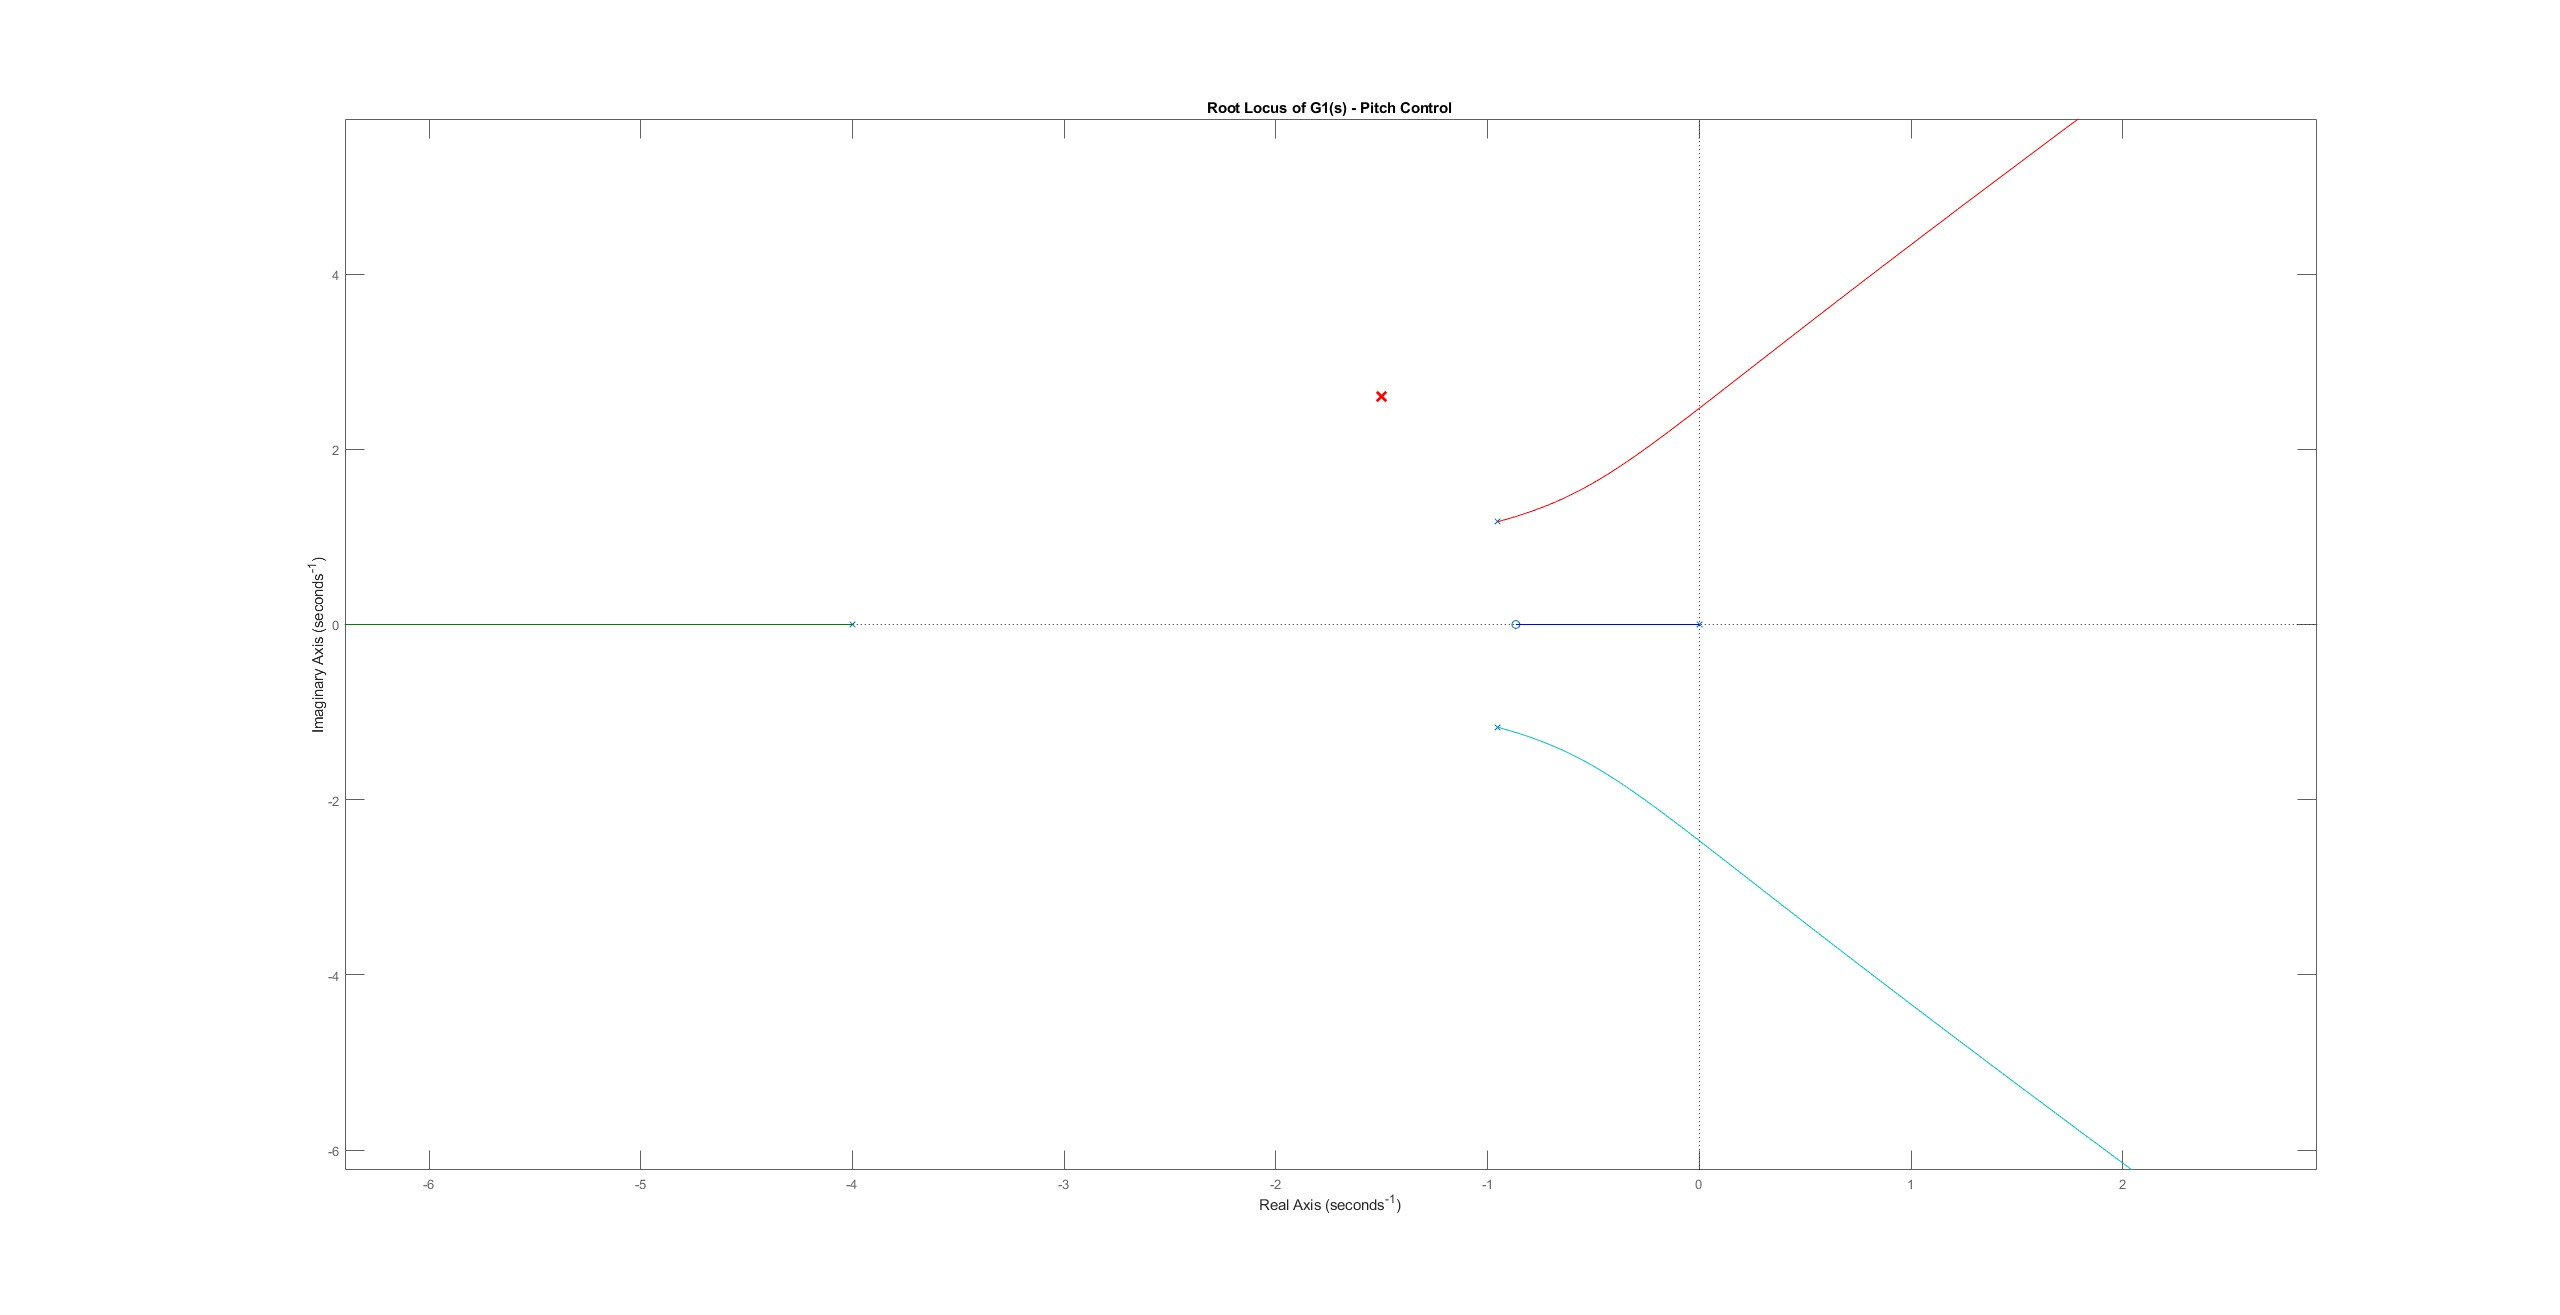
\includegraphics[width=1.0\textwidth]{pictures/Auotpilot/Task3.jpg}
\end{figure}

We can recall the equation of transfer function $G_1(s)$ in Equation 2.11. The root locus of $G_1$ has been plotted along side the complex number $s_1$. However, the complex number does not lie upon a branch of the root locus. This complex number must lie on a branch for the system to function correctly as they represent the location of the system's closed-loop poles. This is why in following tasks, the location of a compensating zero is found. When all the criteria are met, a compensating zero will move the branches of the root locus so that the complex number will lie upon them. 

Task 6 acts a check for this, as it outputs the root locus plot of transfer function $G_2 (s_1)$, Equation 2.16 shows it's mathematical representation. The important difference between $G_1 (s)$ and $G_2 (s_1)$ is that $G_2 (s_1)$ has been compensated with a new zero. This results in the the plot shown in Figure 2.4.
\begin{figure}[H]
    \caption{The Root Locus of $G_2(s_1)$ - Pitch Control}
    \label{fig:task6_result}
    \centering
    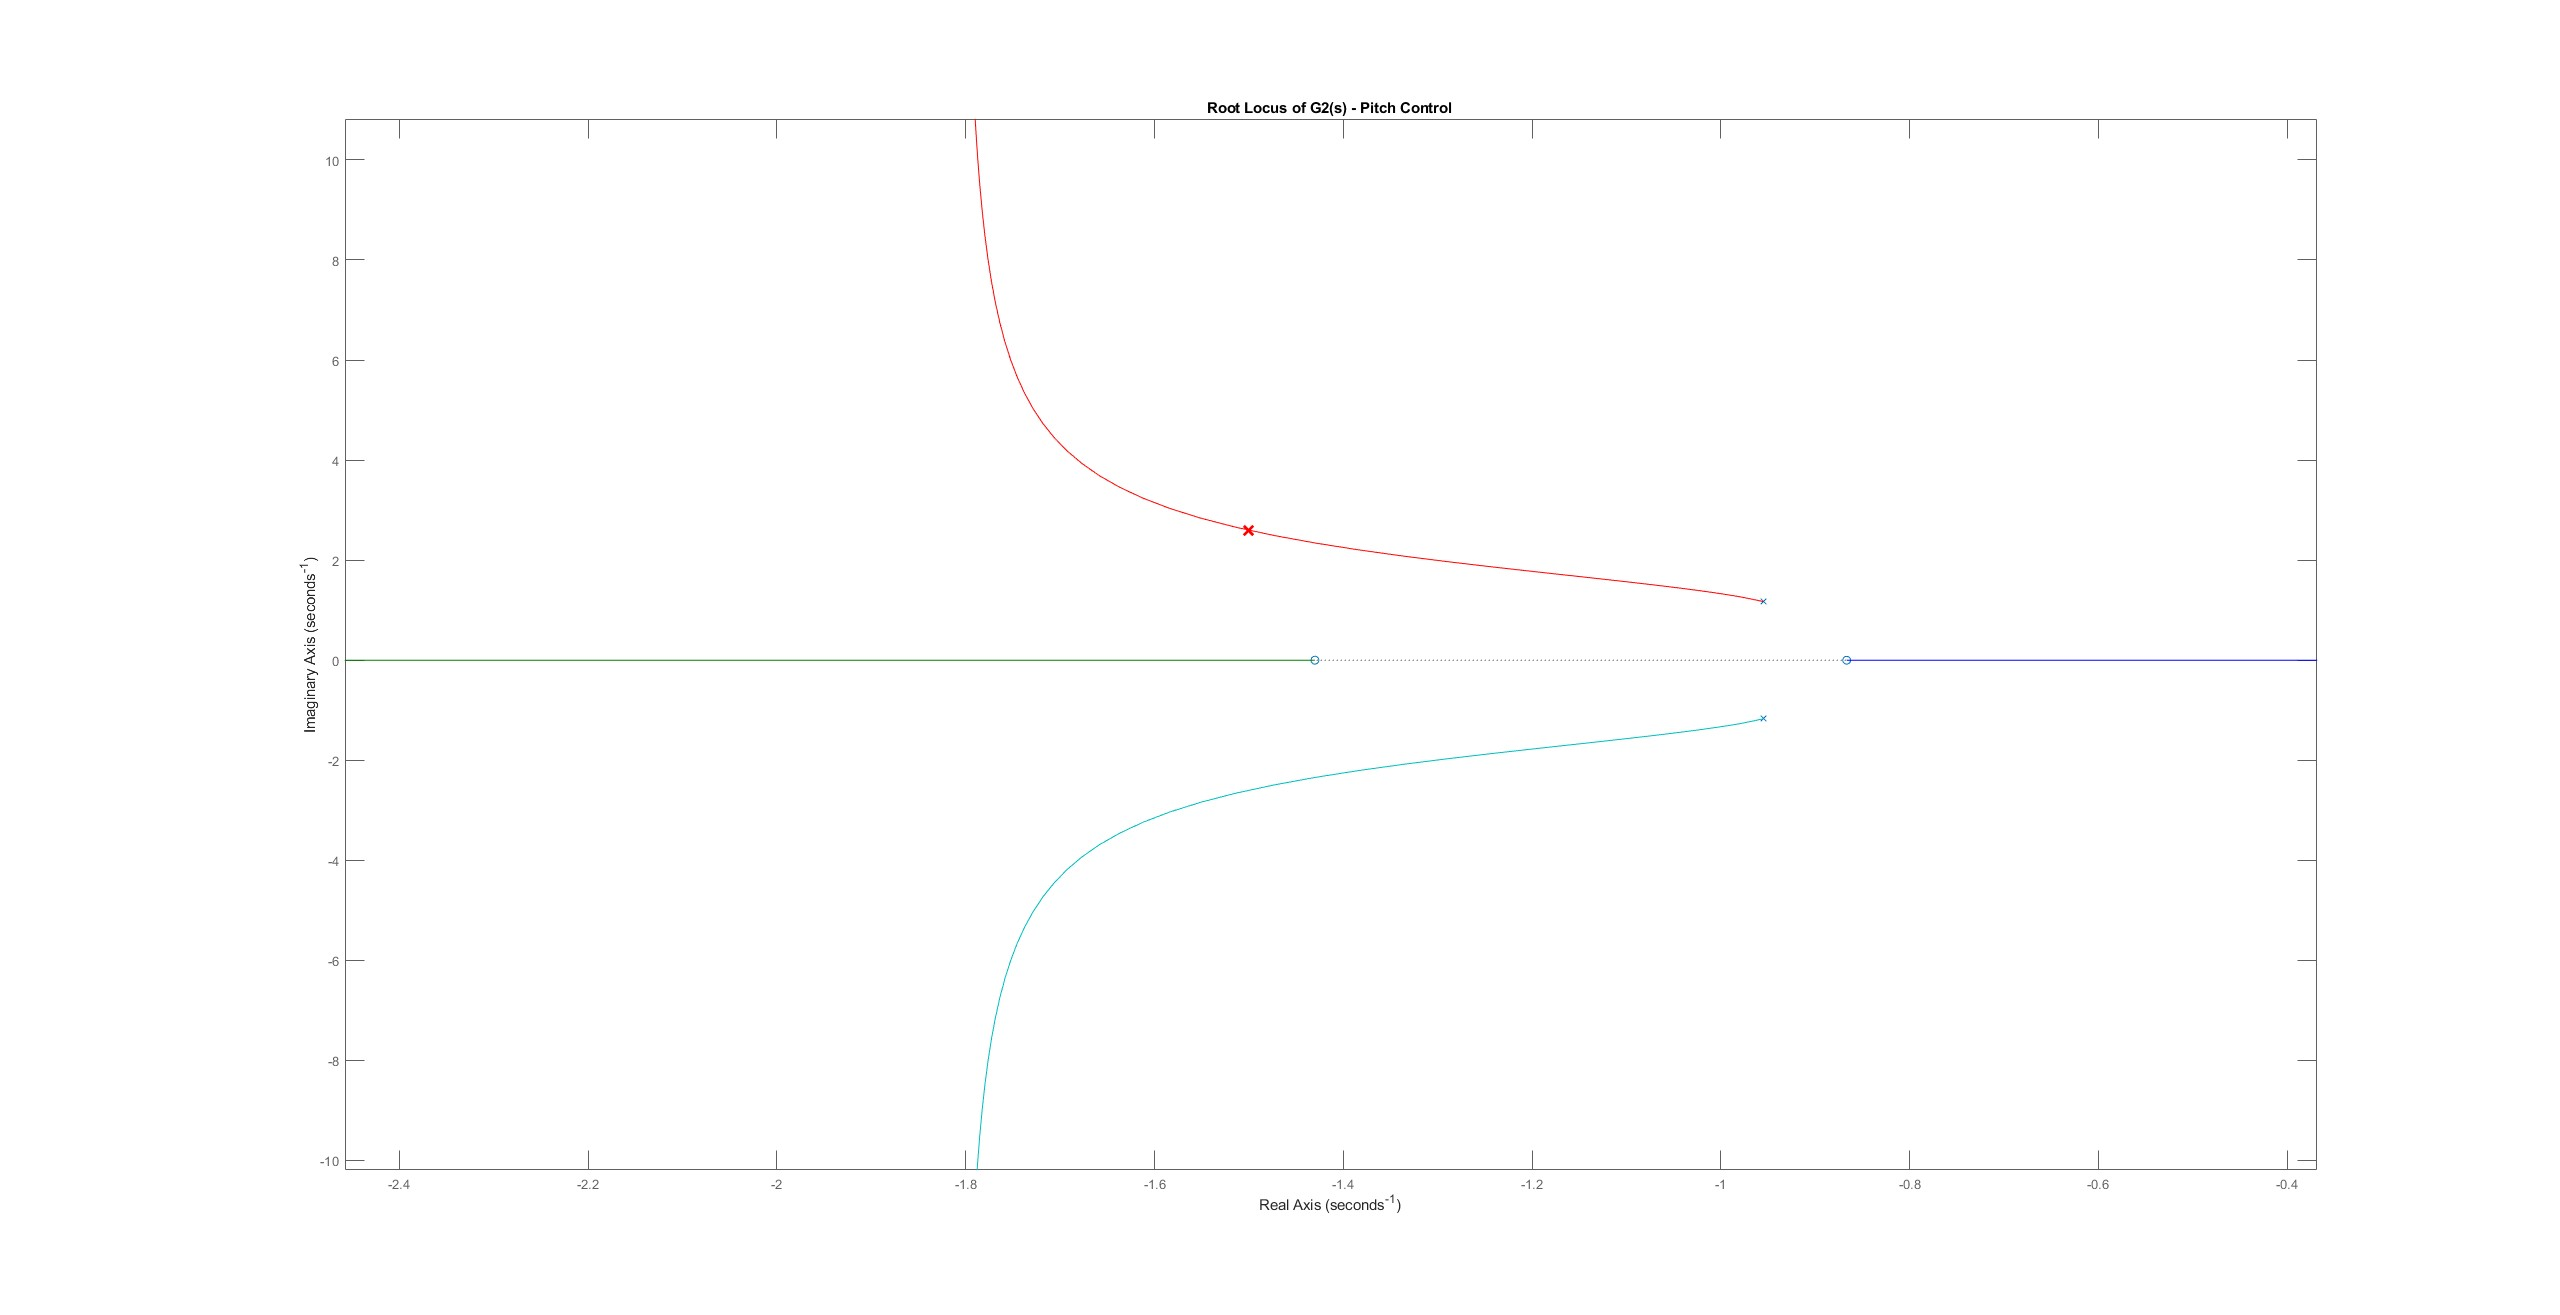
\includegraphics[width=1.0\textwidth]{pictures/Auotpilot/Task6.jpg}
\end{figure}
As seen in Figure 2.4, the root locus plot now intersects with the complex number $s_1$. This means that an acceptable closed-loop pole of the system has been found. Therefore, the step response of the pitch attitude system can be plotted. For this particular simulation, the aircraft experiences a $5^{\degree}$ change to it's pitch attitude. The output of this step response is seen in Figure 2.5.
\begin{figure}[H]
    \caption{Step Response of Pitch Attidude System.}
    \label{fig:task8_result}
    \centering
    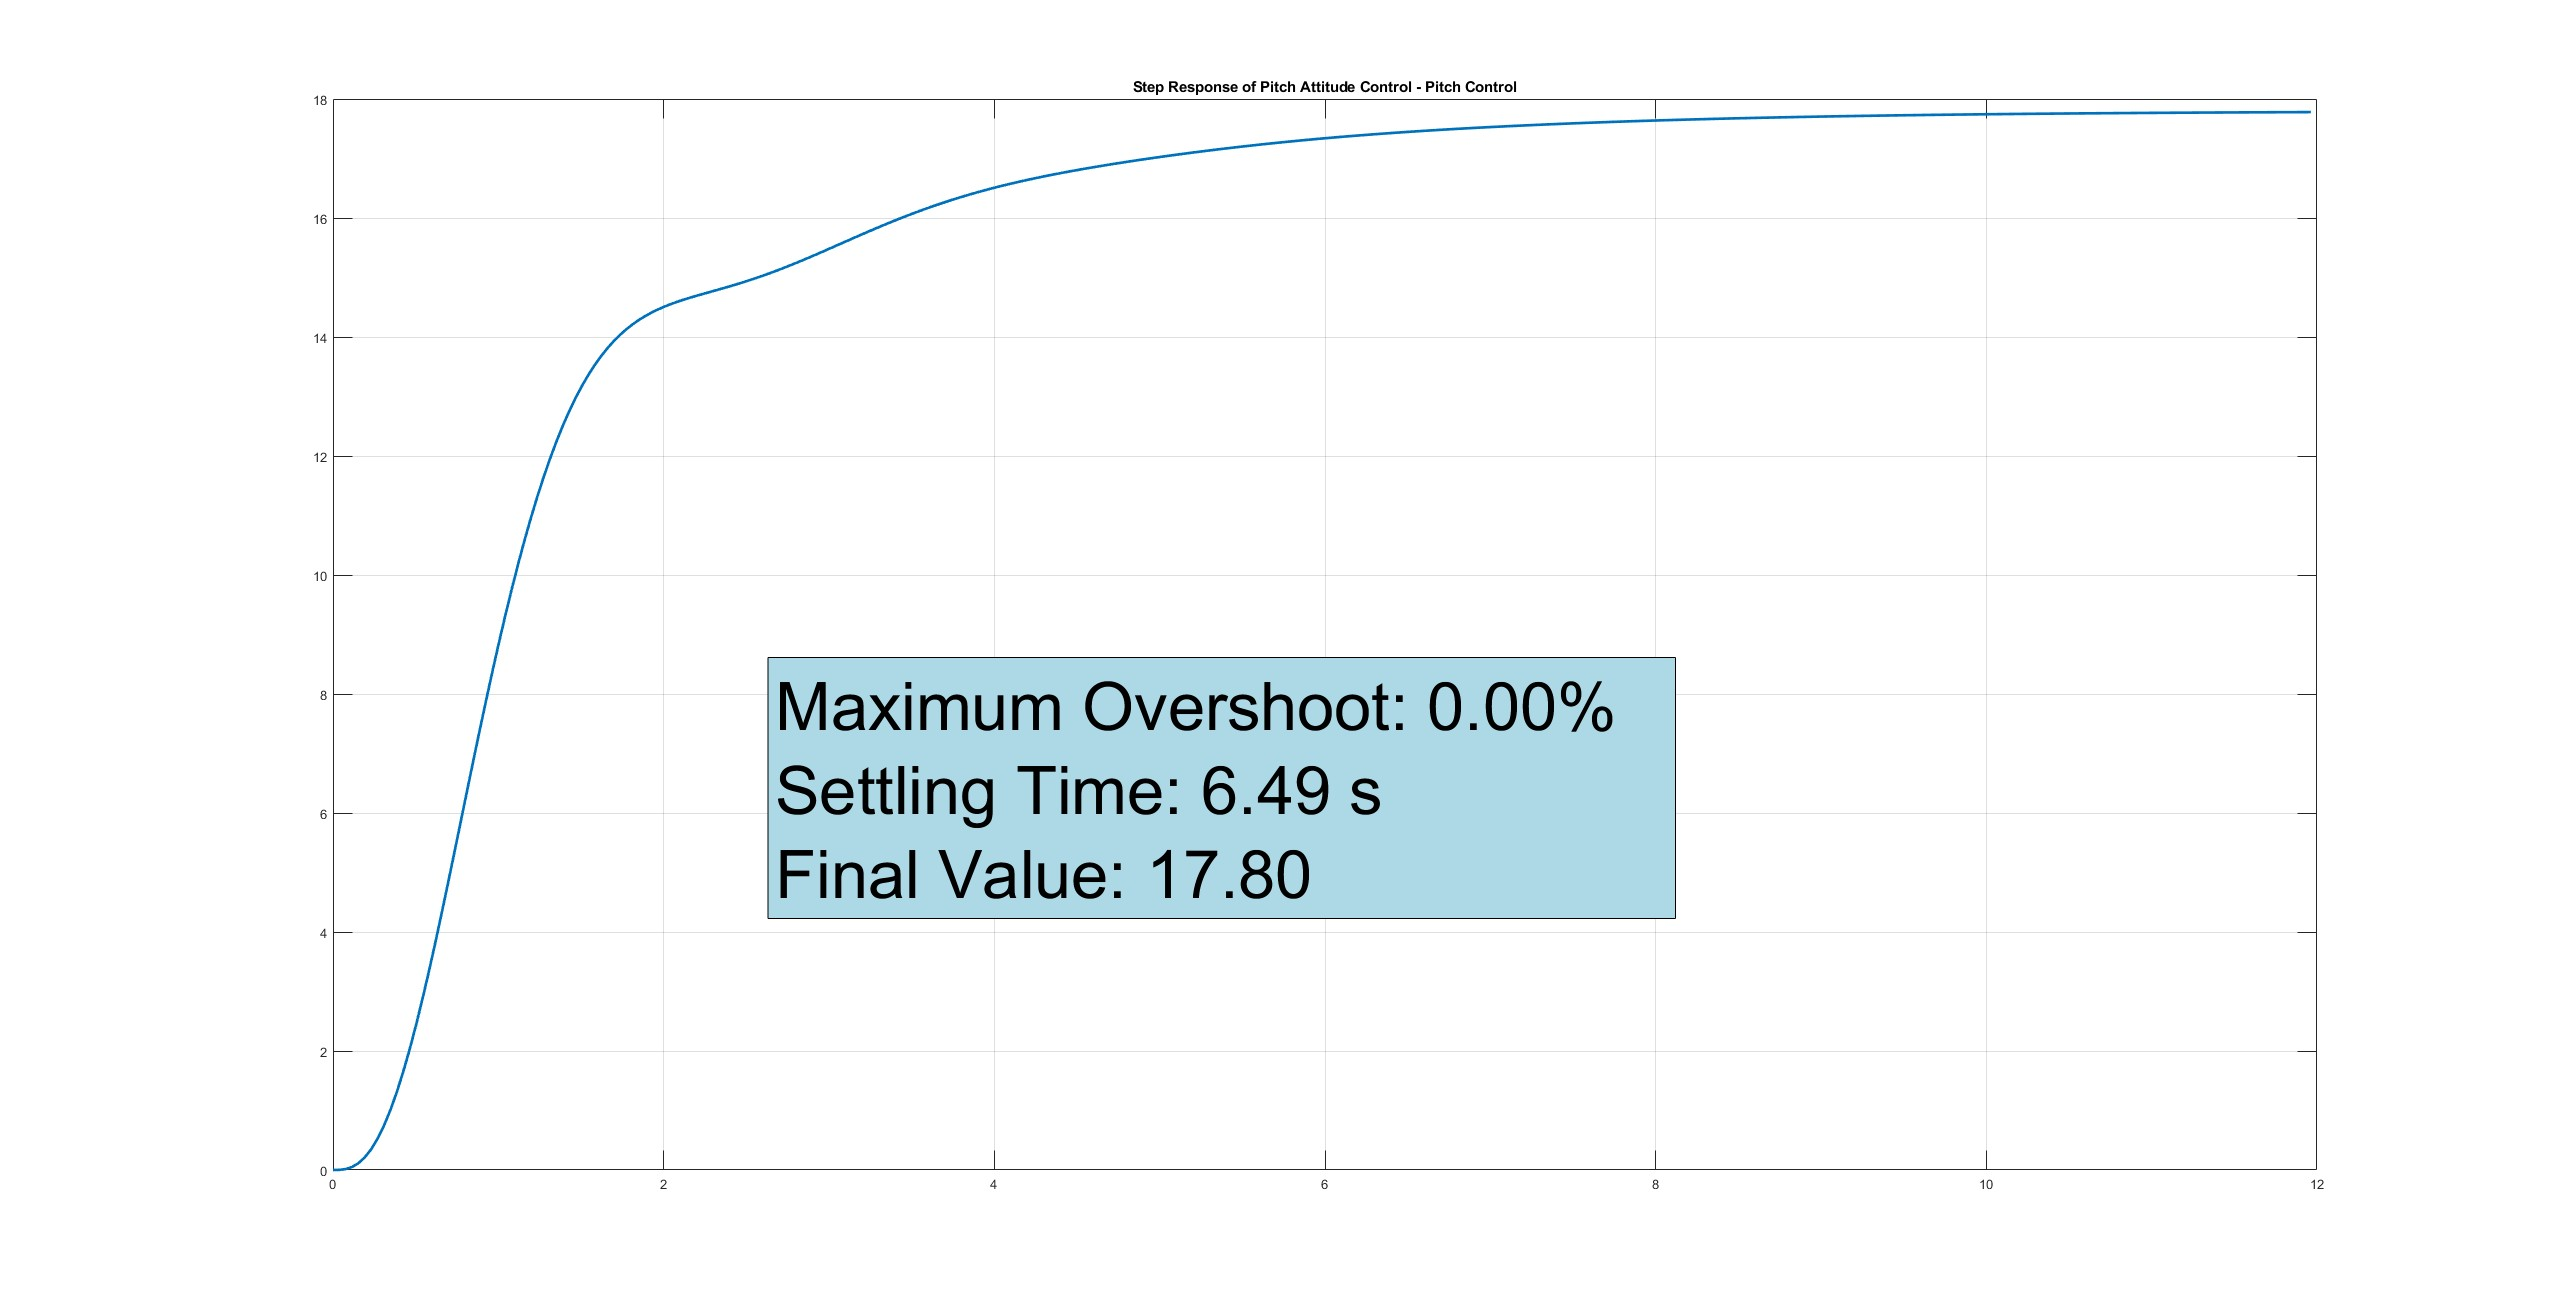
\includegraphics[width=1.0\textwidth]{pictures/Auotpilot/Task8.jpg}
\end{figure}
Figure 2.5 shows that the pitch control system responds to the $5^{\degree}$ change by sending a pitch correction command to the altitude hold system after 6.49 seconds. The pitch needed to correct is $17.8^{\degree}$. All tasks from this point onwards are for the altitude hold section. 

Tasks 11 and 14 are identical to tasks 3 and 6 in terms of their basic function. However, the root locus is designed for transfer function $G^*$ which is defined in Equation 2.18. Therefore, the initial root locus plot is produced, for complex number $s_2$, as seen in Figure 2.6. 
\begin{figure}[H]
    \caption{Root Locus Design for $G^*$.}
    \label{fig:task11_result}
    \centering
    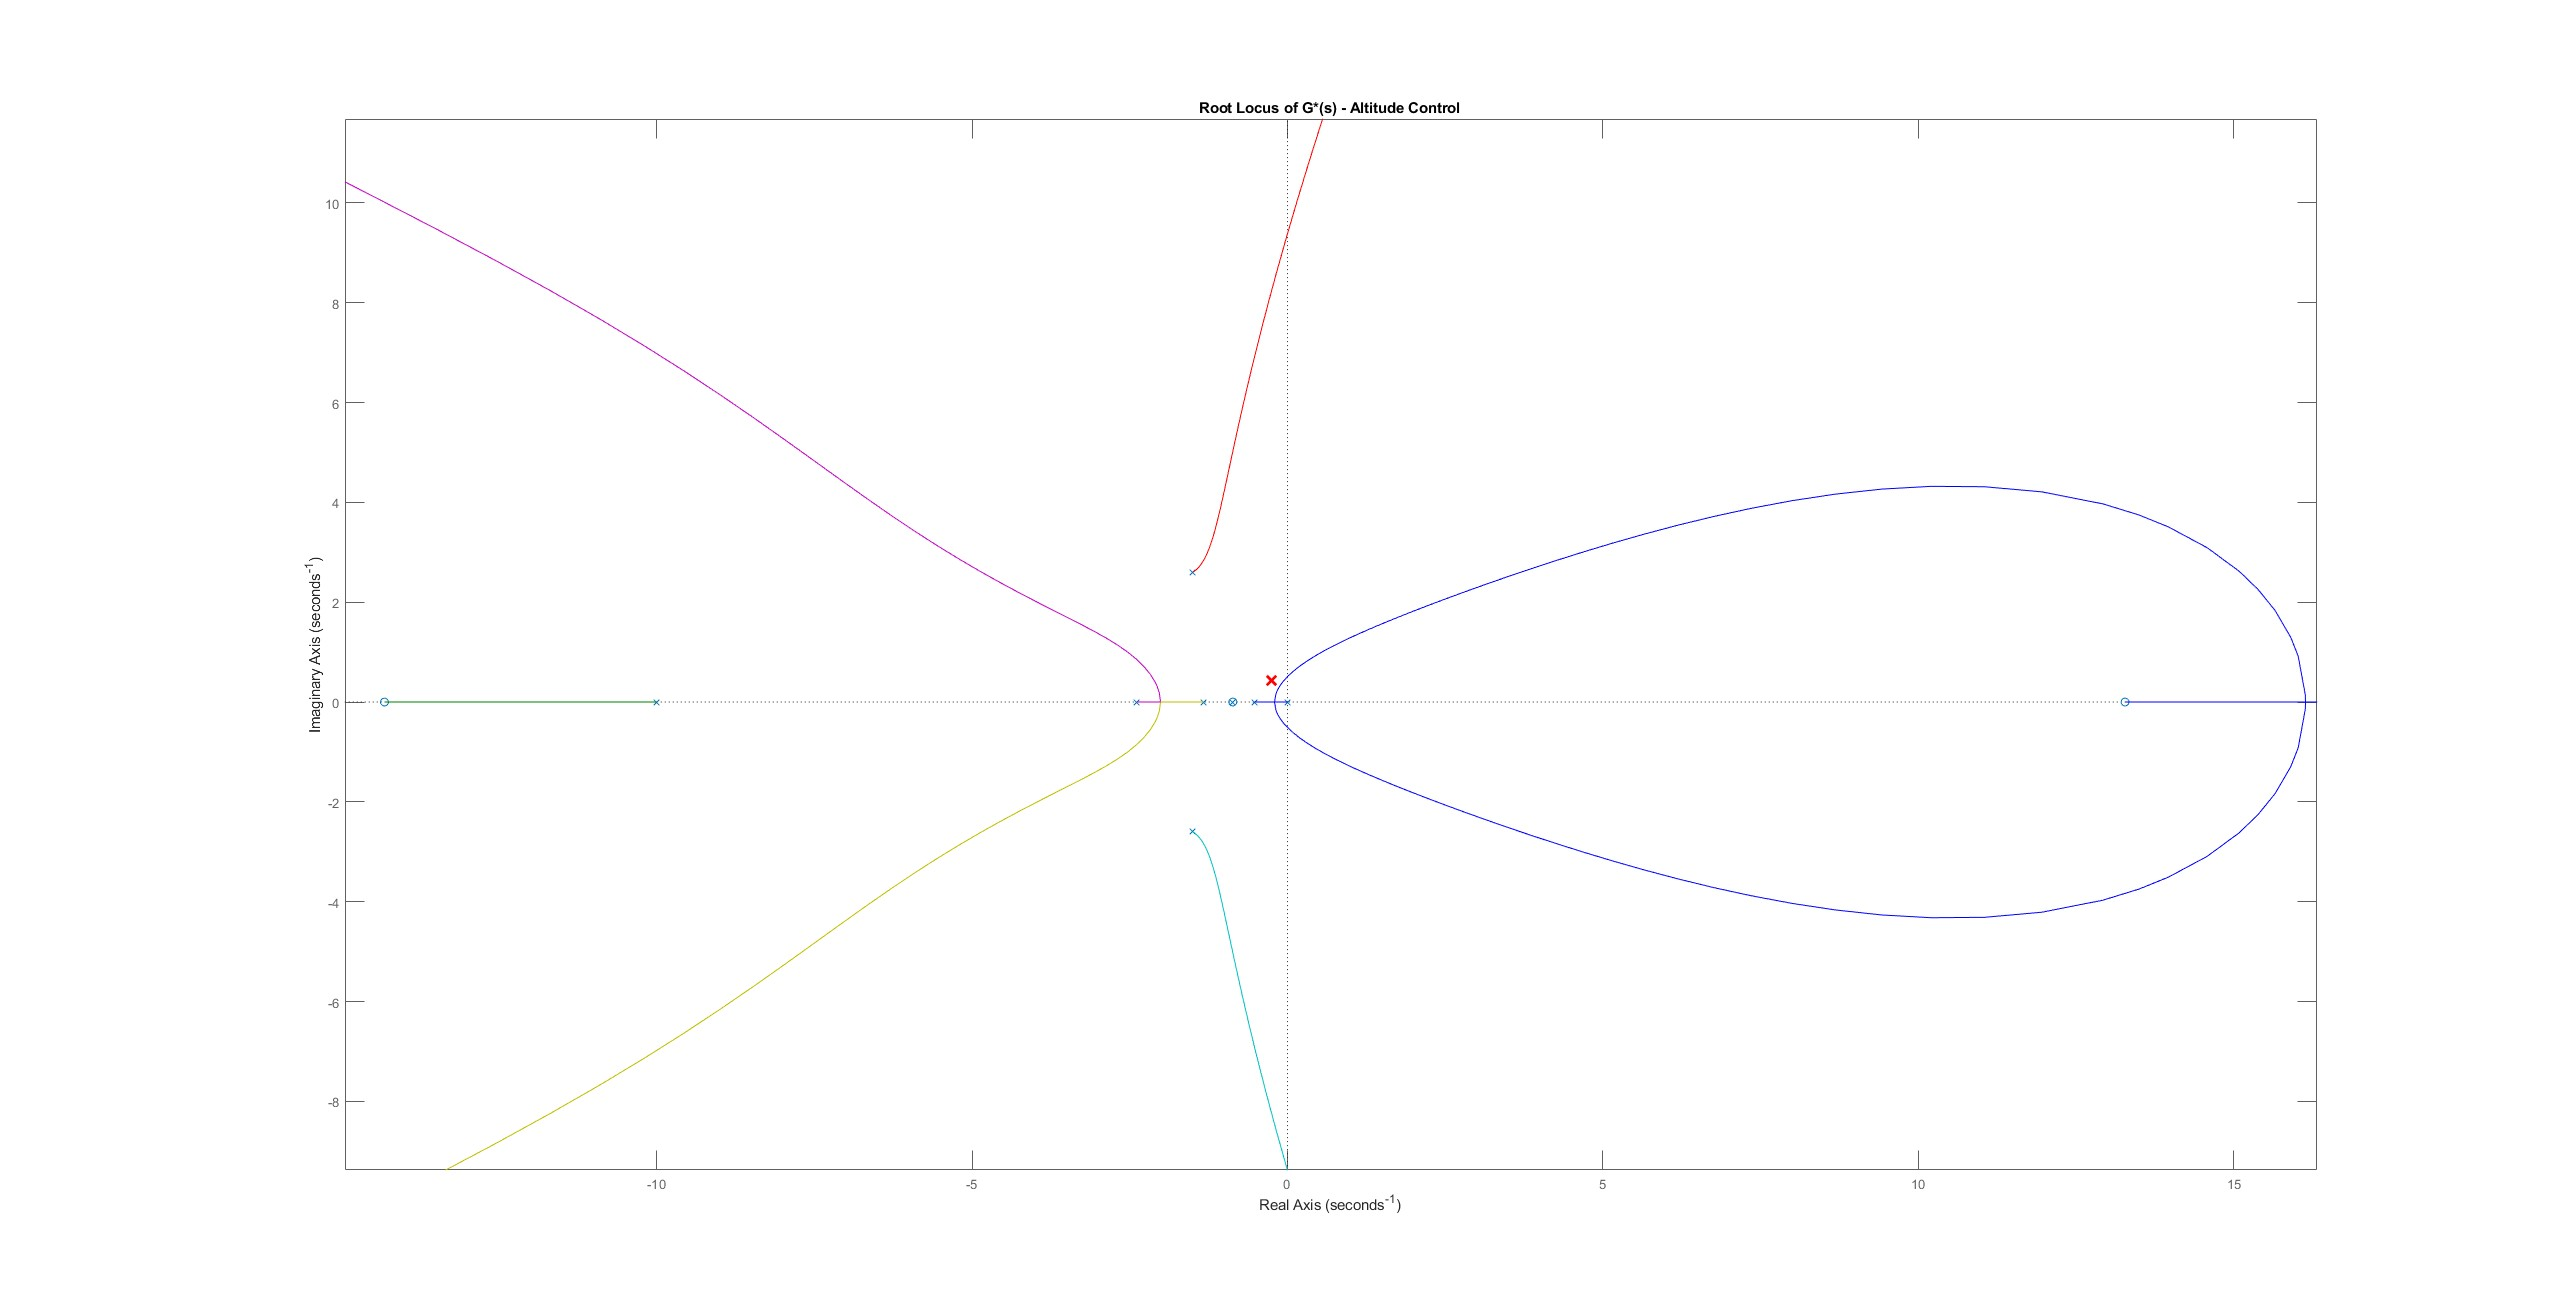
\includegraphics[width=1.0\textwidth]{pictures/Auotpilot/Task11.jpg}
\end{figure}
Just as in task 3, the complex number does not lie on a branch for the root locus design. Therefore, by the method outlined in the theory, it is moved onto a branch, in an identical method to task 6. The result of task 14 can be seen in Figure 2.7
\begin{figure}[H]
    \caption{Root Locus Design for $G_3(s_2)$.}
    \label{fig:task14_result}
    \centering
    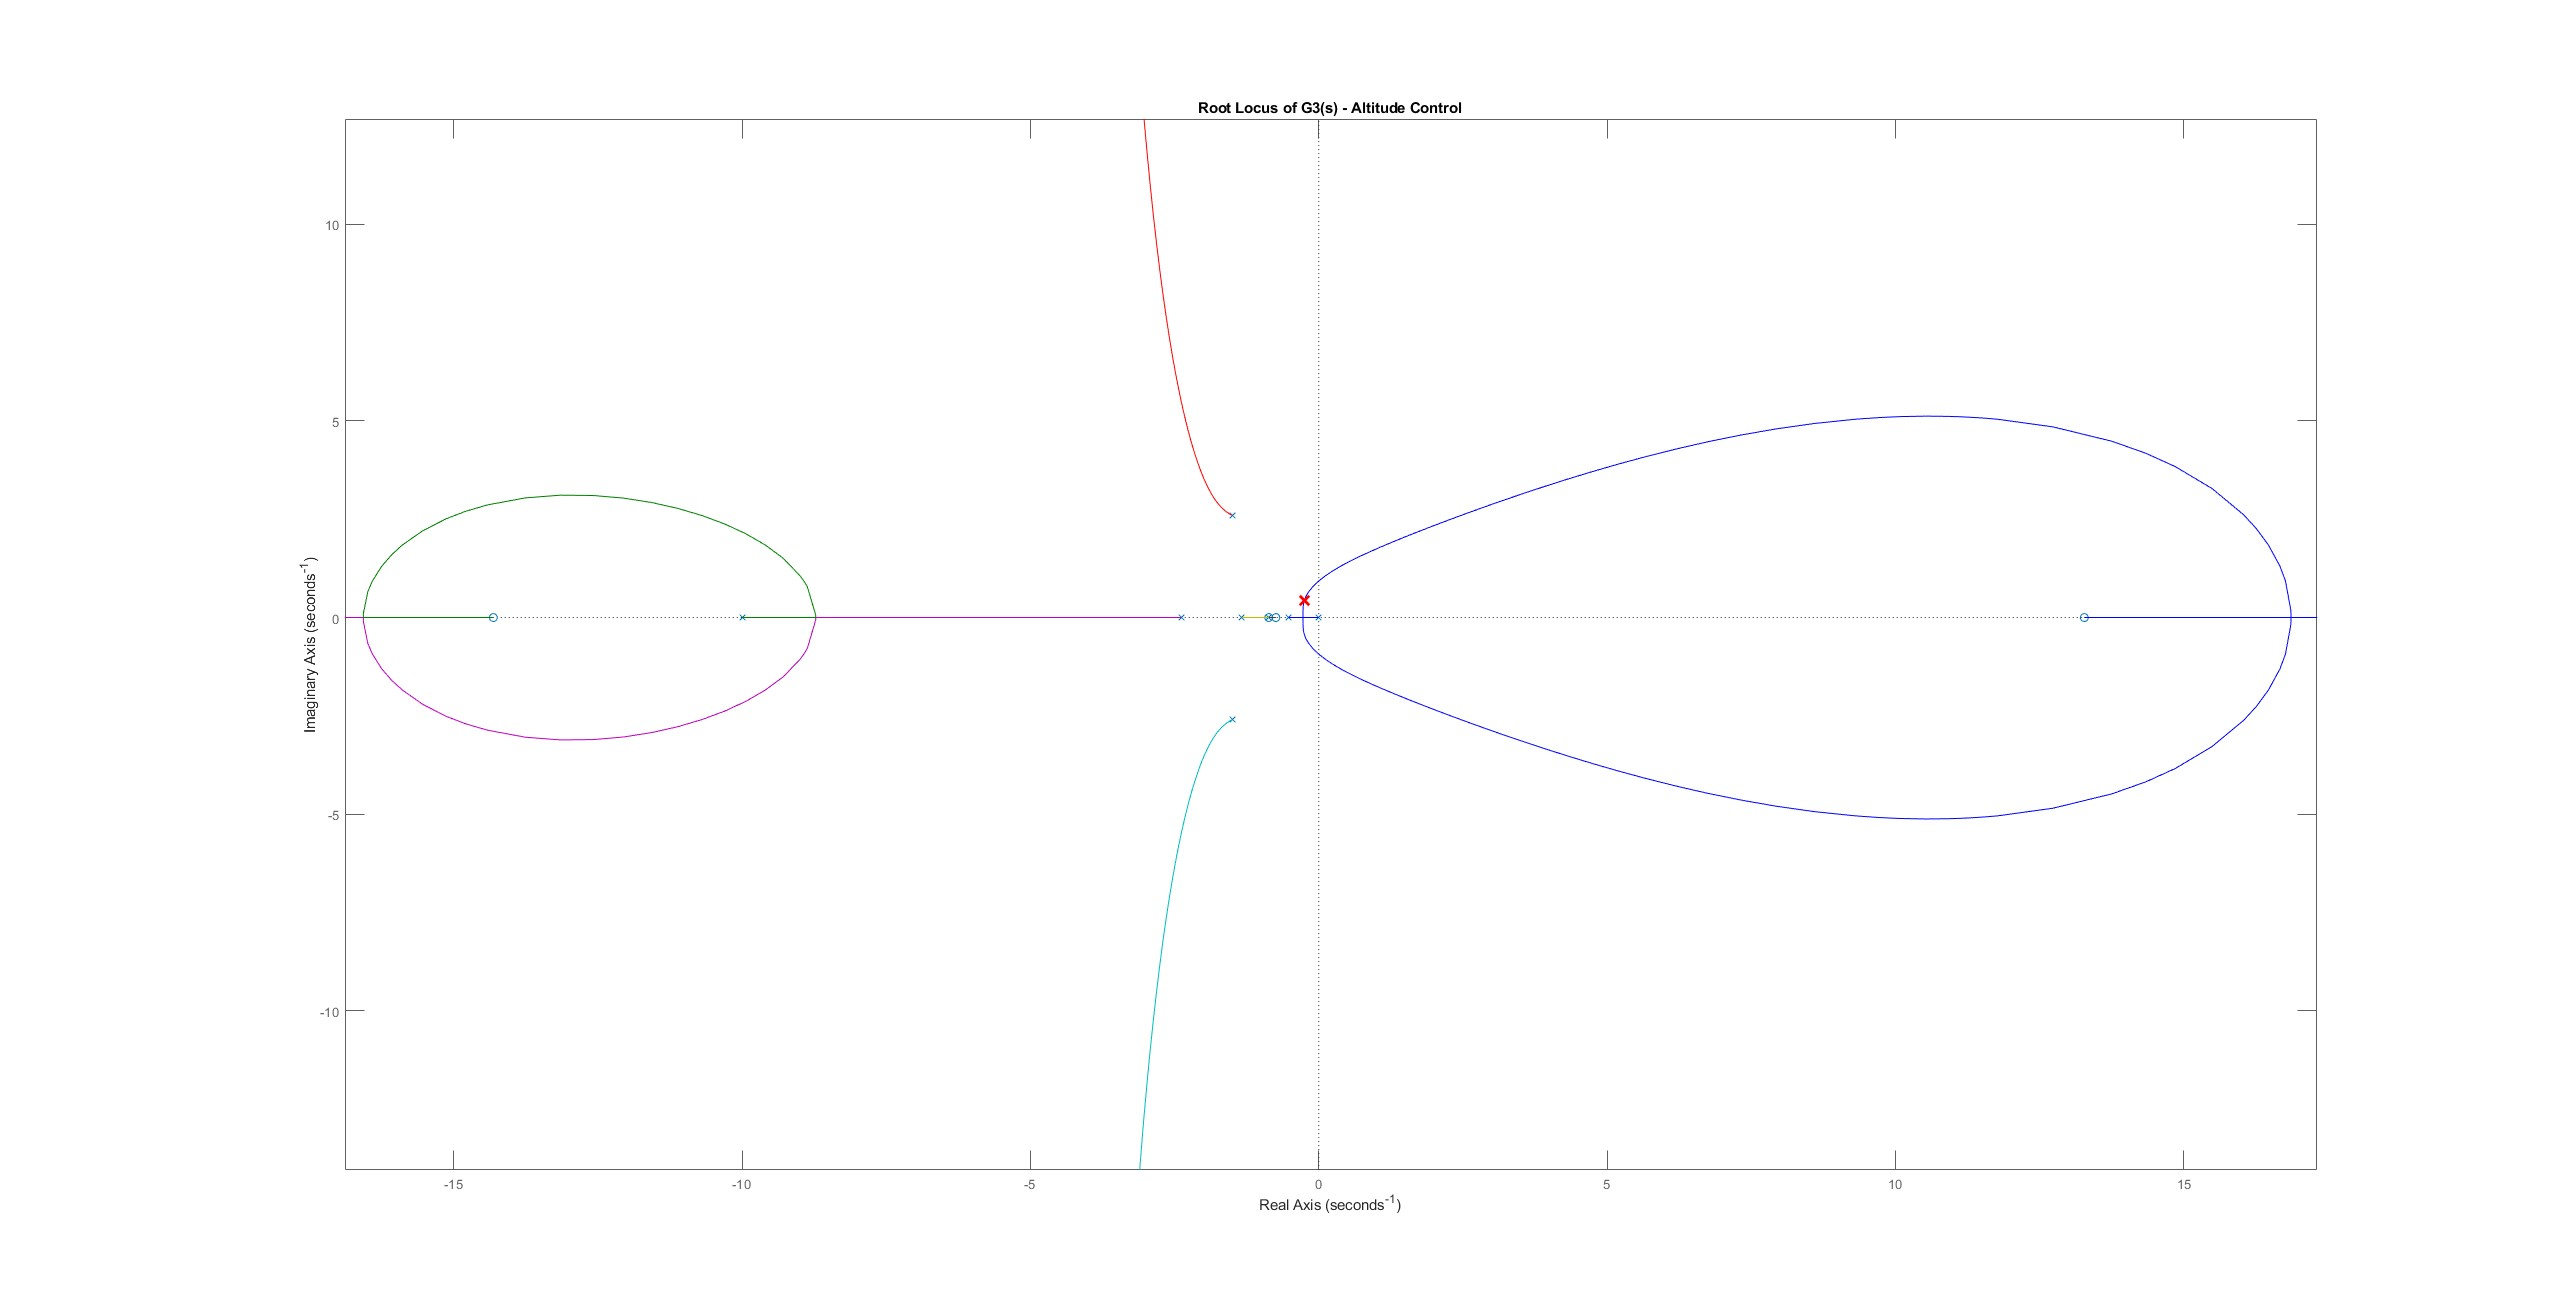
\includegraphics[width=1.0\textwidth]{pictures/Auotpilot/Task14.jpg}
\end{figure}
This means that the final design has been completed for the altitude hold system. Therefore, the step response can be plotted in task 17. The following simulation shows the response, assuming the aircraft experienced  an altitude change of $50m$ due to the pitch change discussed in task 8. The step response can be seen in Figure 2.8.
\begin{figure}[H]
    \caption{Step Response of Altitude Hold System.}
    \label{fig:task17_result}
    \centering
    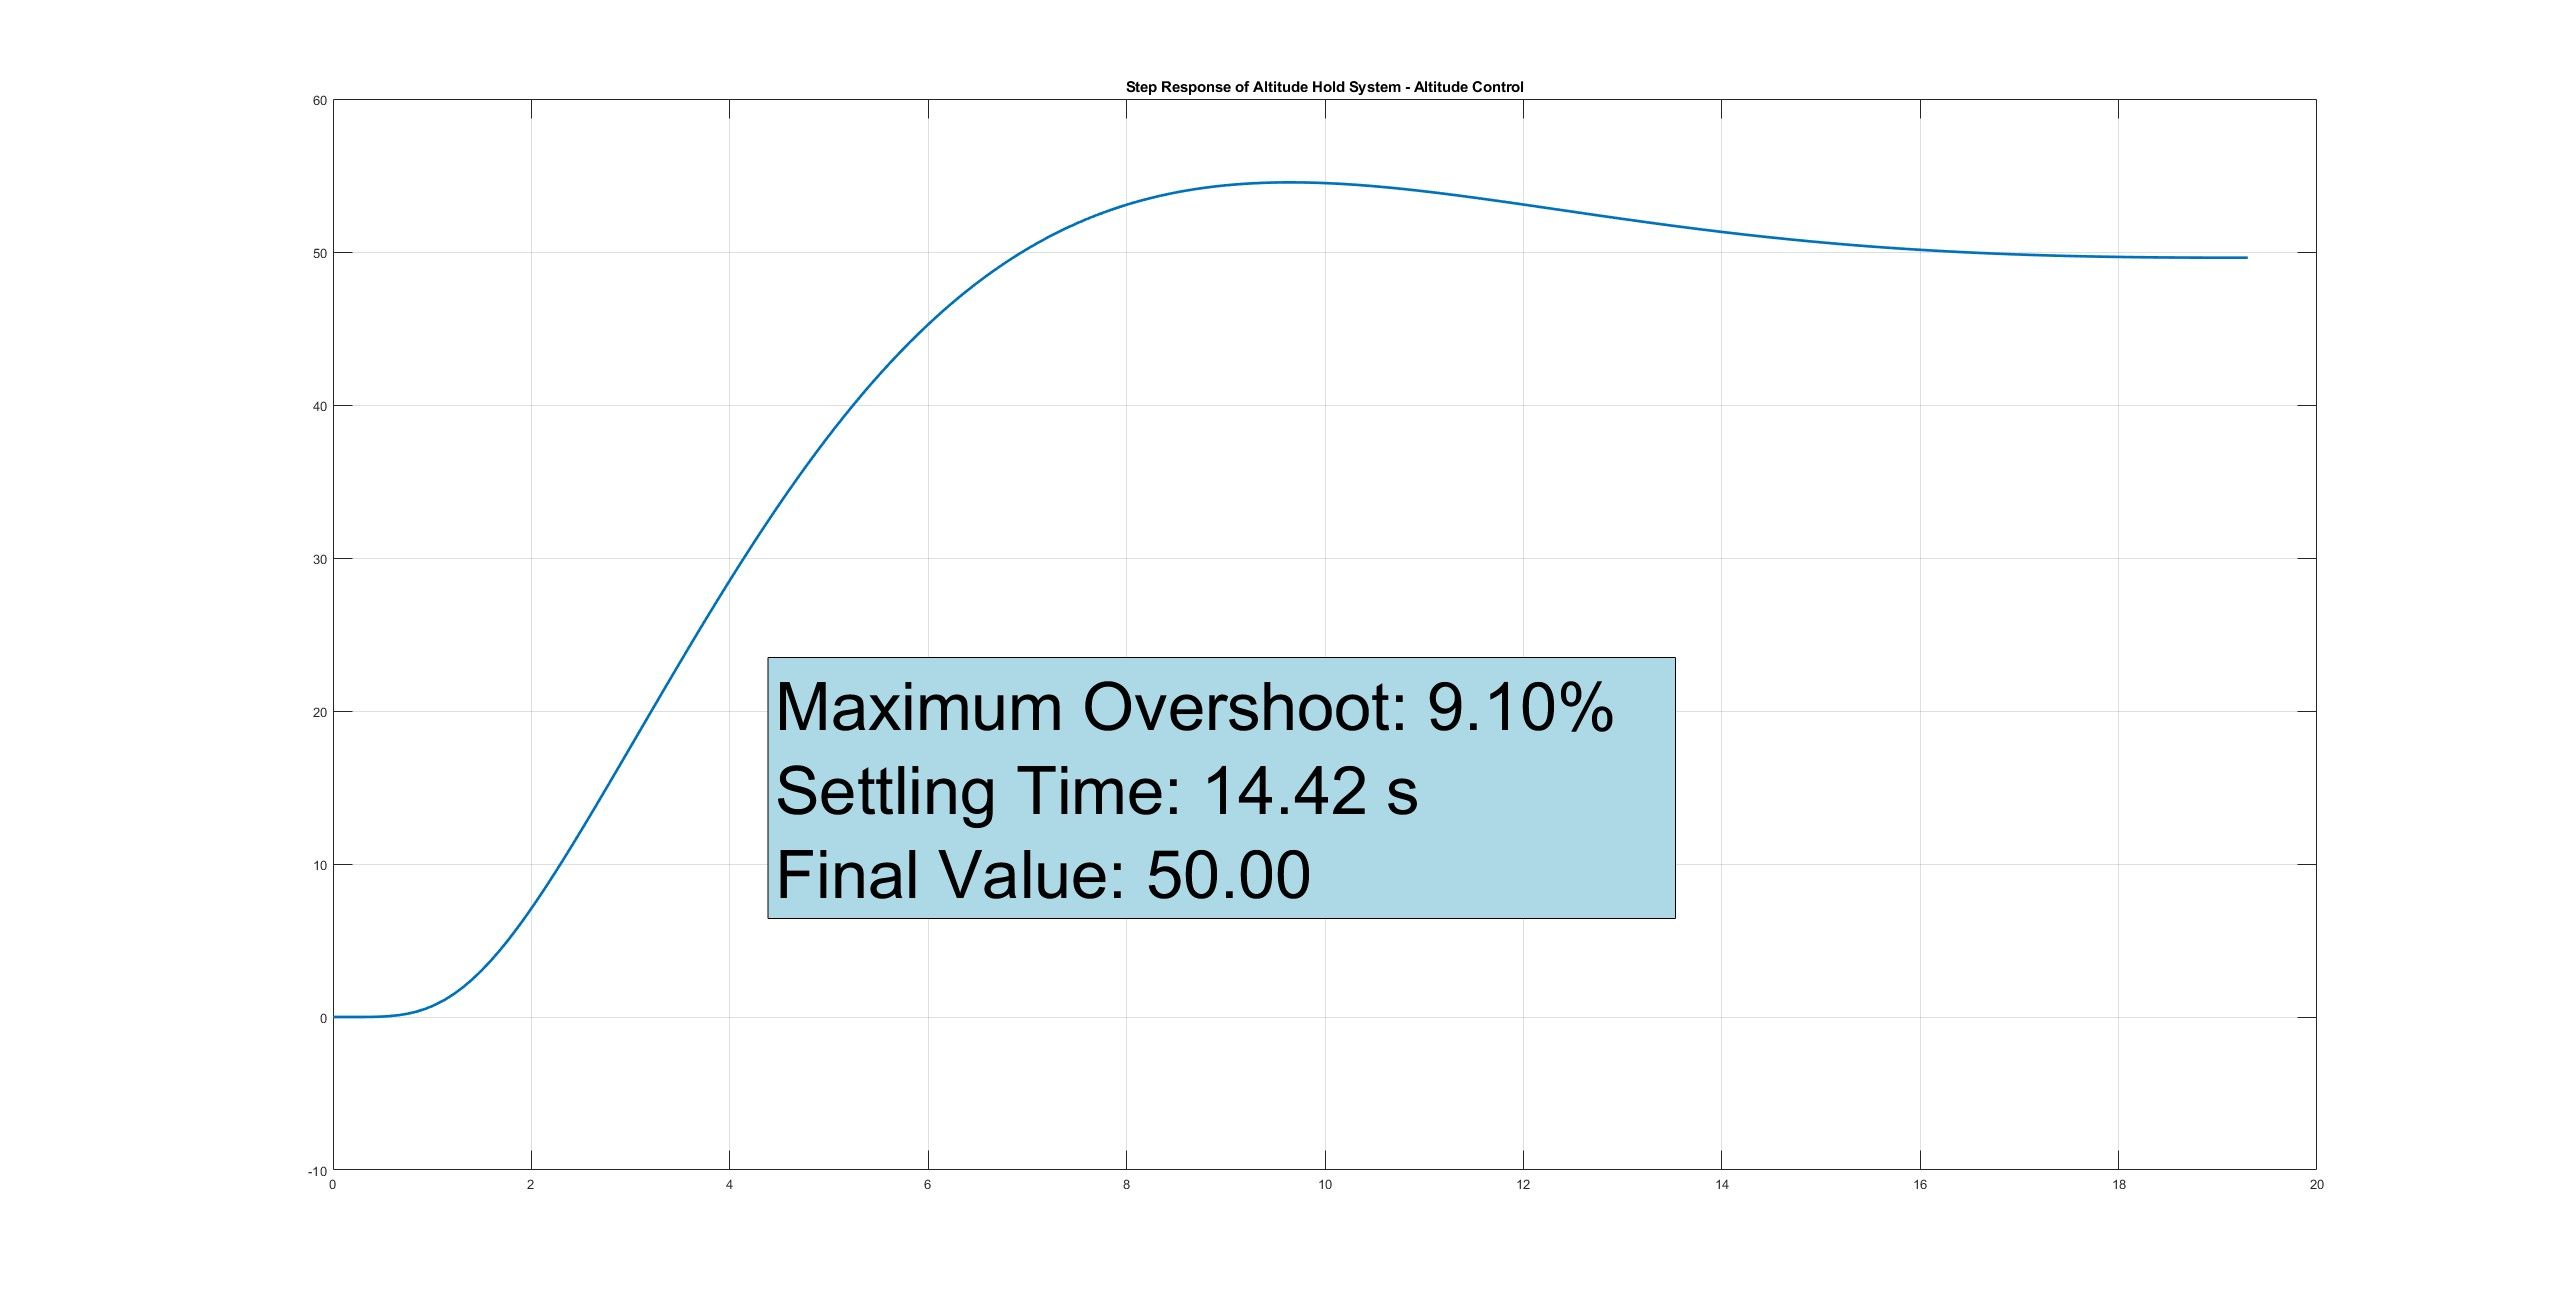
\includegraphics[width=1.0\textwidth]{pictures/Auotpilot/Task17.jpg}
\end{figure}
As seen in this step response, after 14.42 seconds, the aircraft has returned exactly to it's original height (the difference between the altitude change and final value is zero). There is a slight oscillation, as the aircraft initially over-corrects before returning to the original value. 
\subsection{Discussion}
Before discussing the performance of the altitude hold system as a whole, its vitally important to mention the design steps, especially the root locus design. Primarily, this can bee seen in Tasks 3 and 6 for the inner loop and Tasks 11 and 14 for the outer loop, these relate to Figures 2.3, 2.4, 2.6 and 2.7 respectively. 
These figures successfully show how a compensator can be identified by physically moving the root locus branch to lie up on the position of complex numbers $s_1$ and $s_2$ (Equation 2.8), which is determined based on two control parameters; the Damping Ratio and the Natural Frequency. Changing these parameters would result in an Altitude Hold system with a very different performance. 
However, the most important results obtained are thanks to Tasks 8 and 17, which produce Figures 2.5 and 2.8 respectively. 
First of all, the result from Figure 2.5 (Task 8) will be discussed. Figure 8 shows the step response for the pitch attitude system, namely the response of a system when a $5^{\degree}$ pitch change is experienced by the aircraft. The response successfully meets the design criteria as it responds in a fast (6.49 seconds) and stable (zero overshoot) manner. This is exactly what is required for a successful altitude hold system as the inner loop must respond quickly and efficiently to pitch commands, so that altitude corrections can be made in a timely manner. The correcting pitch angle has been determined as $17.8^{\degree}$ and once this is known, the autopilot systems can execute the correcting pitch motion, which will have an impact on the altitude of the aircraft. 
Task 17 and Figure 2.8 discuss how the altitude changes due to this correcting pitch angle previously mentioned. The simulation has been run assuming a step change of 50m in height. The plot in Figure 2.8 successfully meets the design criteria as the aircraft responds in a safe manner, returning to the original altitude after 14.42 seconds. As discussed previously, the altitude response will be significantly slower than the pitch response, this is intentional to avoid excessive oscillations, which creates a more comfortable experience for passengers onboard an aircraft. There is however one oscillation, which can be seen both in the plot response, but also as the maximum overshoot is 9.10\%. This means that the aircraft initially over-corrects before returning to the original altitude. This likely occurs due to a time lag in the correcting the pitch angle once again to maintain the original altitude.     
\subsection{Conclusions} 
In summary, the design of the simple altitude hold system was successful. A mathematical model was created inside of the MATLAB environment and simulations were run to show how this model would handle sudden changes in pitch for an aircraft. This model of course offers a completely ideal simulation, assuming the aircraft's elevators and actuators are working perfectly and the aircraft only experiences one sudden change in pitch, not several small changes in quick succession. However, within the scope of this investigation the model performed as expected, matching up with all the requirements for an altitude hold system for aircraft.  
\newpage
\section{Appendix}
\addcontentsline{toc}{subsection}{List of Figures}
\listoffigures
\addcontentsline{toc}{subsection}{List of Tables}
\listoftables
\addcontentsline{toc}{subsection}{List of Equations}
\listofmyequations

\addcontentsline{toc}{subsection}{Autopilot Script Output}
\textbf{Autopilot Script Output}
\begin{lstlisting}[language=MATLAB]
The phase of G2 at s1 is: 3.1416 radians
The angle criterion has been satisfied for G2 at s1 - the phase is approximately pi.
The poles of G_theta_c are:
  -1.5000 + 2.5981i
  -1.5000 - 2.5981i
  -2.3867 + 0.0000i
  -0.5226 + 0.0000i

The zeros of G_theta_c are:
   -0.8667

The phase of G3 at s2 is: 3.1416 radians
The angle criterion has been satisfied for G3 at s2 - the phase is approximately pi.
The poles of G_altitude are:
  -9.9994 + 0.0000i
  -1.5453 + 2.6332i
  -1.5453 - 2.6332i
  -2.6391 + 0.0000i
  -0.9830 + 0.0000i
  -0.8667 + 0.0000i
  -0.2653 + 0.3325i
  -0.2653 - 0.3325i

The zeros of G_altitude are:
   13.2767
  -14.3131
  -10.0000
   -0.8667
   -0.7437
\end{lstlisting}

\newpage
\addcontentsline{toc}{subsection}{References}
\printbibliography

\end{document}